% !TEX TS-program = xelatex
% !TEX encoding = UTF-8 Unicode


\documentclass[AutoFakeBold]{LZUThesis}
%\usepackage{subfigure}
\usepackage{graphicx}
\usepackage{subfloat} 
\usepackage{diagbox}

\begin{document}
%=====%
%
%封皮页填写内容
%
%=====%

% 标题样式 使用 \title{{}}; 使用时必须保证至少两个外侧括号
%  如: 短标题 \title{{第一行}},  
% 	      长标题 \title{{第一行}{第二行}}
%             超长标题\tiitle{{第一行}{...}{第N行}}

\title{{基于改进U-net的小样本图像分割}}



% 标题样式 使用 \entitle{{}}; 使用时必须保证至少两个外侧括号
%  如: 短标题 \entitle{{First row}},  
% 	      长标题 \entitle{{First row}{ Second row}}
%             超长标题\entitle{{First row}{...}{ Next N row}}
% 注意:  英文标题多行时 需要在开头加个空格 防止摘要标题处英语单词粘连。

\entitle{{Few-Shot Learning for Semantic Segmentation }{based on improvements to U-net}}
% \entitle{{Few-Shot Learning for Semantic Segmentation} {based on Deep Learning}}

% 我曾见证无数人不改这几项,或者不改完全……,下一个会不会是你?
\author{郁严贵}
\major{计算机科学与技术}
\advisor{刘振宇}
\college{信息科学与工程学院}
\grade{2018级}



\maketitle
\thispagestyle{empty}

%======%
%诚信说明页
%授权说明书
%======%
% 如果超出边界,可以调整签字的宽度,现在是40,如果你不用,把下面的注释就好

% 你的签名
\mysignature{
    % \raisebox{-5pt}{
    % 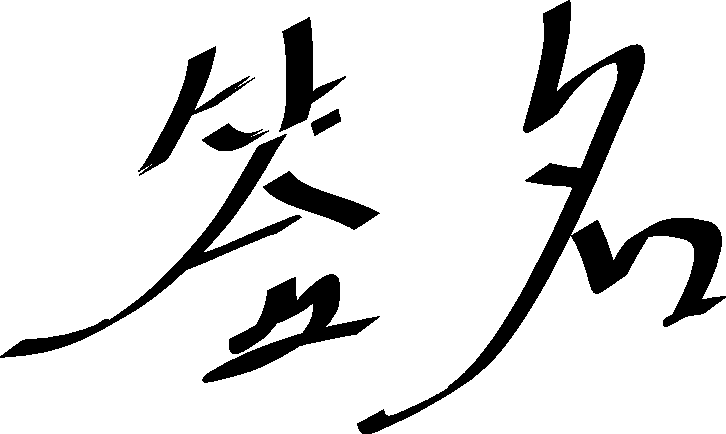
\includegraphics[width=40pt]{signature.pdf}
    % }
}
% 你手写的日期
\mytime{
    % \raisebox{-5pt}{
    % 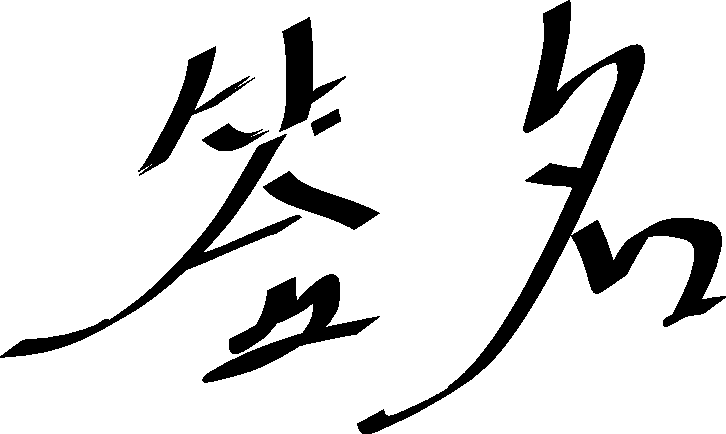
\includegraphics[width=40pt]{signature.pdf}
    % }
}
% 老师的手写签名
\supervisorsignature{
    % \raisebox{-5pt}{
    % 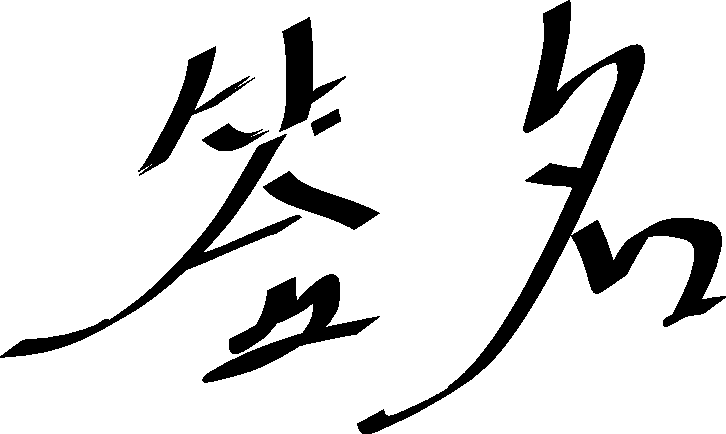
\includegraphics[width=40pt]{signature.pdf}
    % }
}
% 老师手写的时间
\teachertime{
    % \raisebox{-5pSt}{
    % 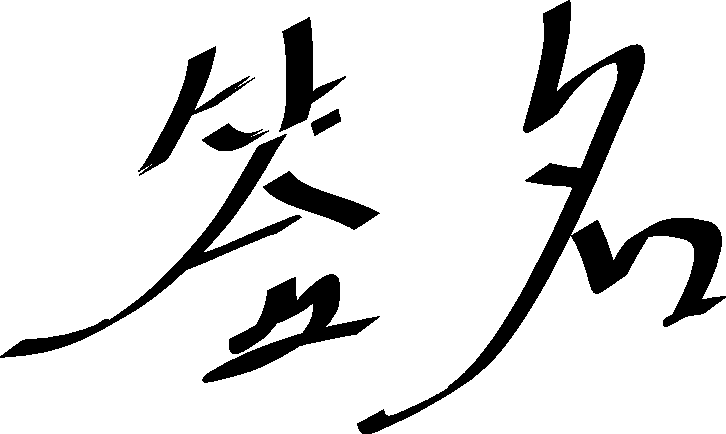
\includegraphics[width=40pt]{signature.pdf}
    % }
}
% 老师手写的成绩
\recommendedgrade{
    % \raisebox{-5pt}{
    % 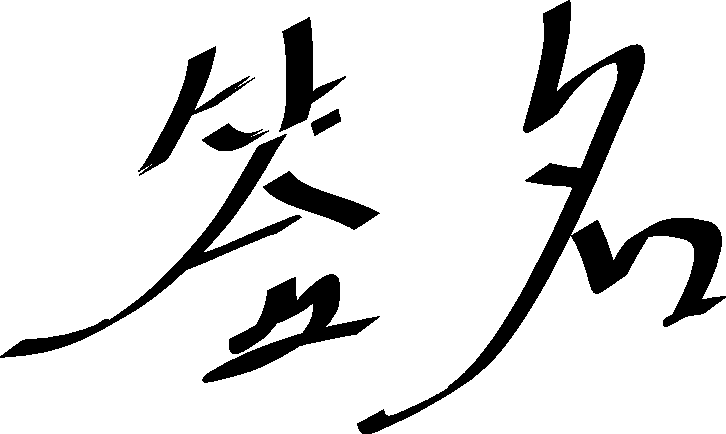
\includegraphics[width=40pt]{signature.pdf}
    % }
}
\makestatement

% %=====%
% %论文(设计)成绩
% %=====%
% % 下面这些注释掉可以去掉成绩、评语什么的
\supervisorcomment{}

\recommendedgrade{}

\supervisorsignature{
    \raisebox{-10pt}{
        % 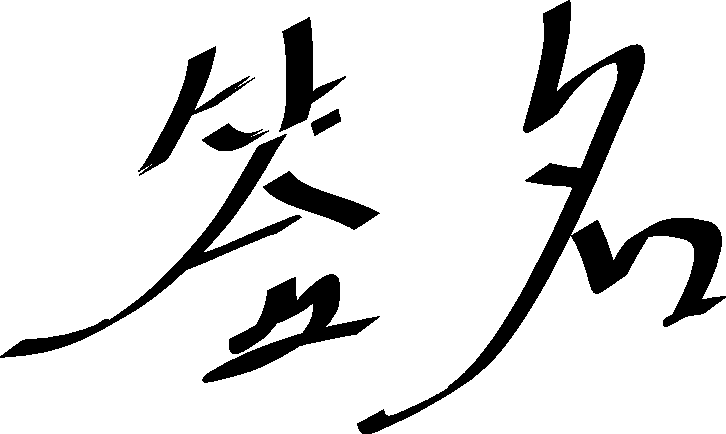
\includegraphics[width=60pt]{signature.pdf}
    }
}

\committeecomment{}

\finalgrade{}
% % 上面这些注释掉可以去掉成绩、评语什么的

% \Grade %这一句才是成绩页
\Grade %这一句才是成绩页

\frontmatter



%中文摘要
\ZhAbstract{
    近年来,依赖于大量数据训练的深度学习模型在诸多领域获得成功的应用。但在疾病诊断、欺诈识别、故障检测等领域,在实际中往往难以获得大量的训练数据。因此,在可获得的数据量不足的情况下,如何让模型可以在有限的数据上得到更好的训练结
    果,对图像实现更准确的分割效果,是小样本图像分割要解决的问题。

    U-net是图像分割领域流行的网络模型架构,在所需的训练集较少便可以取得比较好的图像分割效果。本论文研究如何对传统的U-net网络结构进行改进,以使网络模型更好的解决小样本图像分割问题。本论文的主要研究工作如下:

    ​	第一,针对训练数据不足的问题,采用水平翻转、旋转、缩放、颜色变换等技术对训练数据集进行数据增强。通过对比分析多种增强操作,选择适用于图像分割任务的方案。

    ​	第二,针对在小样本条件下,图像边缘分割效果不理想的问题,改进损失函数对边缘分割效果的权重分配方法,提升网络模型对图像边缘分割的敏感性,改善图像分割的效果。

    ​	第三,分析U-net网络模型在小样本图像分割任务下的不足,针对不足对网络模型做出改进,并通过对比实验证明了改进的U-net模型更适合小样本图像分割任务。

    综上,本文研究了数据增强、设计损失函数和改进U-net模型对于图像分割结果的影响。通过实验验证了上述研究工作可以有效的改善在小样本条件下,图像分割的效果。}
{深度学习,卷积神经网络,图像分割,U-net,小样本学习,数据增强}

%英文摘要
\EnAbstract{
    In recent years, deep learning models that rely on large amounts of data for training have been used successfully in many fields. However, in areas such as disease diagnosis, fraud recognition and fault detection, it is often difficult to obtain large amounts of training data in practice. Therefore, with the insufficient amount of available data, how to make the model can get better training results on limited data and achieve more accurate segmentation results on images is the problem to be solved for few-shot image segmentation.

    U-net is a popular network model architecture in the field of image segmentation, which can achieve better image segmentation results with less training set required. This thesis investigates how the traditional U-net network architecture can be improved to make the network model better for few-shot image segmentation problems. The following are the main contents to be studied in this thesis:

    Firstly, to address the problem of insufficient training data, data enhancement is applied to the training dataset using techniques such as horizontal flip, rotation, scaling and color transformation. By comparing and analyzing multiple enhancement operations, a scheme suitable for the image segmentation task is selected.

    Secondly, to address the problem of unsatisfactory image edge segmentation under few-shot conditions, the weight assignment method of the loss function on the edge segmentation effect is improved to enhance the sensitivity of the network model to image edge segmentation and improve the effect of image segmentation.

    Thirdly, the shortcomings of the U-net network model in the few-shot image segmentation task are analyzed, the improvements made to the network model in response to the shortcomings, and the improved U-net model is demonstrated to be more suitable for the small-sample image segmentation task through comparative experiments.

    In summary, this thesis investigates the effects of data enhancement, design of loss function and improved U-net model on image segmentation results. It is verified that the above research work can effectively improve the results of image segmentation under few-shot conditions.}
{Deep learning, convolutional neural network, image segmentation, U-net, few-shot learning, data augmentation }

%生成目录
\tableofcontents
%文章主体
\mainmatter


% \Intro{
%     其实我推荐绪论写在正文里!!作为第一章

%     这里是绪论,也可以说是引言\\

%     重要的事情说一遍吧。。。注意啊,如果你编译以后\textbf{没有参考文献},那是因为编译需要四步走:
%     $$XeLaTeX -->BibTeX --> XeLaTeX-->XeLaTeX$$

%     没看懂?百度去,这都不会你就开始去用latex写论文了。。。
%     算了,给你找几个教程吧\\
%     \url{http://blog.sina.com.cn/s/blog_4ddef8f80100kn21.html}\\
%     \url{https://blog.csdn.net/qq_36718092/article/details/89361629}\\


%     额,或许还没看懂,小白的话还是用vscode吧,配置简单一些,

%     \url{https://zhuanlan.zhihu.com/p/38178015}

% }


% =======正文从第一章开始
\setcounter{chapter}{0}

\chapter{绪论}
\section{研究背景与意义}
进入21世纪以来,随着计算机的快速发展以及大数据时代的到来,在日常生活中与网络中产生了大量的数据,这为深度学习的发展提供了基础。近年来,深度学习取得了极大的成功,并且人工智能与深度学习的研究方向也异常火热。

当前,在计算机视觉(Computer Vision, CV)和自然语言处理(Natural Language Processing, NLP)等领域,深度学习都取得了极大的成功。作为计算机视觉领域的一个重要研究方向,图像分割将图像中感兴趣、关注的区域划分切割出来,去除掉无关的背景噪声。作为图像分析和处理的重要环节,图像分割在很多领域都有着广泛的应用,如在人脸识别中将人脸信息与背景区分开来,在行人检测中需要分割出每个行人实例,在医学领域中进行医学图像的分割。

随着深度学习的进展,应用深度学习理论在图像分割这一问题上表现出了卓越的性能,当前提出来很多方法来解决图像分割这一问题。其中,基于卷积神经网络(Convolutional Neural Network, CNN)的方法在图像分割问题上取得了非常好的效果。但是,CNN网络模型通常需要大量的训练数据。目前,深度学习的成功主要得益于大量的训练数据。然而大量可获得的训练数据在有些问题和情境下是很困难,或者不可能的。对图像分割的准确标注的代价是昂贵的,需要耗费大量的人力成本和精力。在图像分割这一问题下,对图像的标注需要精确到像素级的分类上,这是一件耗时且困难的任务。这导致在很多情境下,如医学图像和工业领域中,缺乏大量的可以获得的标注数据用于模型的训练。

深度学习往往需要大量的训练数据进行训练,从大量的数据中提取信息,才能训练得到效果比较好的模型。与此相对,人类具有很强的学习能力,“举一反三”的推理能力,只需要少量的样本,便可以取得很好的学习效果。如何在可获得的训练数据不足的情况下,进行更有效的图像分割,这便是小样本图像分割要研究的问题。小样本学习的目标是在训练数据不足的情况下,在测试集上取得更好的表现效果。因此,研究在小样本这一情景下,如何实现基于深度学习网络模型从小样本中取得更好的学习效果,对于图像实现更好的分割效果,更符合实际要面临的实际情况,具有重要的现实和理论意义。


\section{研究现状综述}
本文的研究内容在图像分割与小样本学习两个方向开展,并将小样本学习的理论研究成果应用于图像分割这一问题。因此,在国内外的研究现状中,本文将从图像分割的研究现状和小样本学习的研究现状进行梳理。
\subsection{图像分割研究现状}
卷积神经网络(Convolutional Neural Network, CNN)是一类强大的、表示性很强的网络,通常用于处理图像数据,基于卷积神经网络的神经网络模型在处理计算机视觉相关任务时表现出非常好的效果。经典的卷积神经网络如LeNet\textsuperscript{\cite{lecun1989handwritten}}、AlexNet\textsuperscript{\cite{krizhevsky2012imagenet}}会在卷积层后会加上全连接层,将卷积层提取的特征图映射为一维特征向量输出。这适用于图像分类任务,而对于图像分割任务,可以看作像素级的二分类问题,神经网络的输出大小需要与输入图片的大小相同。如果采用全连接层,则会产生大量的参数,拟合如此多的参数需要大量的数据,同时训练的时间和空间开销将会异常庞大。

2015年,Jonathan Long等提出了全卷积神经网络(Fully Convolutional Network, FCN)\textsuperscript{\cite{long2015fully}},实现了从图像级别的分类到像素级别的分类,从卷积图提取的特征图中恢复得到每个像素所属的类别,解决了图像语义分割的问题,是使用深度学习模型解决图像分割问题的里程碑。在此之后,提出了很多用于解决图像分割问题的模型\textsuperscript{\cite{minaee2021image}}。

2015年,Olaf Ronneberger等提出了U-net网络模型\textsuperscript{\cite{ronneberger2015u}},U-net在FCN基础上进行了改进,将来自下采样阶段的通道特征与上采样的通道特征进行拼接,使通道数增加一倍,同时下采样和上采样分别进行4次,呈对称的结构特征。
2016年,Vijay等提出了SegNet网络\textsuperscript{\cite{badrinarayanan2017segnet}},SegNet是一种全卷积神经网络,用于像素级别的图像分割,通过在最大池化操作时记录位置索引,然后在上采样阶段利用记录的位置索引来恢复信息,降低了内存的消耗量。2017年,何凯明等提出Mask R-CNN\textsuperscript{\cite{he2017mask}},在Faster R-CNN\textsuperscript{\cite{ren2015faster}}的基础上进行了改进,添加了预测目标分割区域的分支,使得Mask R-CNN既可以用于目标检测,又可以用于实例分割。

\subsection{小样本学习研究现状}
当前,对于小样本学习的研究方向主要分为数据处理方向和模型算法方向。
\subsubsection{基于数据增强的小样本学习}
数据处理主要是通过数据增强的方式来对训练数据进行处理,解决训练数据不足的问题。数据增强作为一种有效的扩充训练样本容量的方式,不仅可以用于小样本学习的情况下;在训练数据充足的情况下,也可以进行数据增强,进一步提升模型性能。一个模型的性能除了和网络模型结构本身有关,数据增强在很大程度上也有助于提高一个模型的性能。当前,在图像分类这一问题下,提出了很多数据增强策略\textsuperscript{\cite{shorten2019survey, yang2022image}}。

AutoAugment\textsuperscript{\cite{cubuk2019autoaugment}},从数据中学习数据增强策略,是一种自动数据增强策略。AutoAugment定义了一个搜索空间,包括可以选择的数据增强操作,进行该操作的概率以及图像增强的幅度。通过在搜索空间上进行搜索,得到对应数据增强策略。
RandAugment\textsuperscript{\cite{cubuk2020randaugment}},每次随机的从候选的数据增强操作中选择一些数据增强操作,对数据进行数据增强。有两个超参数,进行图像增强操作的数量N
和图像增强幅度M。
TrivialAugment\textsuperscript{\cite{muller2021trivialaugment}},每次随机的选择图像增强操作和图像增强幅度,对图像进行数据增强。
RandomErasing\textsuperscript{\cite{zhong2020random}},从图像中随机的去除一部分区域,保留图像的标签信息。
MixUp\textsuperscript{\cite{zhang2017mixup}},在图像分类问题中,对每个图像有其对应的标签,mixup随机的将两个图像进行线性组合,同时对它们的标签信息也进行相应的线性组合。



\subsubsection{基于模型的小样本学习}
目前,用于解决小样本学习问题的模型主要可以分为度量学习和元学习\textsuperscript{\cite{赵凯琳2021小样本学习研究综述,李新叶2020基于深度神经网络的少样本学习综述,lu2020learning}}。度量学习通过评估样本与支撑集中的距离,选择度量距离最接近的类别,借助最近邻的思想完成分类。元学习的方法通过学习到的先验知识实现在少量样本上参数的快速更新。
\begin{itemize}[topsep=5pt,listparindent=25pt]
    \item 度量学习
          \par 在数学概念下,度量(又称为距离函数)是衡量一个定义集合中不同元素之间距离的函数\textsuperscript{\cite{shen2014recent}}。度量学习,即相似度学习,是为了评估两个样本之间的距离,从而衡量样本之间的相似程度。\textsuperscript{\cite{bellet2013survey}}度量学习的目标是使得相同类别的样本具有比较大的相似度,而不同类别的样本具有比较小的相似度。目前,度量学习的方法主要应用于图像分类、人脸识别、音乐识别等领域。

          2015年,Koch等人提出了孪生神经网络(siamese neural network)\textsuperscript{\cite{koch2015siamese}},孪生神经网络是一个双路的神经网络,进行单样本图像类别识别,是一种相似度度量模型,用于判断两个样本是否属于同一个类别。训练时,输入是一对样本,通过组合构造不同的样本对进行训练。在预测时,将测试样本与支撑集中进行比较,与支撑集相似度最高的所属类别作为测试样本的类别输出。
          2016年,Vinyals等提出了匹配网络(matching network)\textsuperscript{\cite{vinyals2016matching}},将样本映射到低维向量空间上,计算要分类的样本与带标签样本的相似度,相似度高的作为预测标签输出。
          2017年,Snell等提出了原型网络(prototype nertwork)\textsuperscript{\cite{snell2017prototypical}},认为每个类别存在一个原型,通过将图片映射为向量,对于图片的分类问题变为求与测试样本最接近距离的对应类别原型。
          2018年,Sung等提出了关系网络(Relation network)\textsuperscript{\cite{sung2018learning}},关系网络不采用距离函数来计算样本之间的相似度,而是使用神经网络的方式对距离的度量方式进行学习。

    \item 元学习
          \par
          元学习,即学会去学习(learning to learn)\textsuperscript{\cite{thrun1998learning}}。元学习利用以往的学习知识来帮助新任务的学习,让模型获得学习能力,这种能力可以帮助模型学习到一些元知识。当前深度学习任务针对特定的任务一般需要在数据集上从头开始训练模型,神经网络的参数等都要先进行随机初始化。而元学习可以在当前的模型训练过程之外,通过对在大量的先验任务中学习到的元知识,来帮助模型在新任务上更好更快的学习。元知识包括超参数、神经网络的初始参数等。这符合人类的认知模式,在基于记忆带来的大量先验知识的基础上,对于新的物品只需要少量样本便可以学习到它的特征。

          2016年,Santoro等人提出基于记忆增强的神经网络(memory-augmented neural networks)\textsuperscript{\cite{santoro2016meta}},使用记忆增强的方法来解决单样本学习问题。Santoro提出的神经网络基于神经图灵机(neural Turing machine)\textsuperscript{\cite{graves2014neural}}。神经图灵机既可以进行长时记忆,又可以实现短期记忆。通过神经图灵机学习将样本类型存入记忆的策略,并学习如何用这些类型来进行预测。
          2017年,Munkhdalai等人提出元网络(meta network)\textsuperscript{\cite{munkhdalai2017meta}},元网络包括两个部分,base-learner和meta-learner,在不同的任务中学习元知识,学习不同任务之间的泛化信息时对权重缓慢更新;在新的要处理的任务上实现对权重的快速更新。
\end{itemize}



\section{面临的困难和挑战}
目前的数据增强策略和小样本学习模型主要针对于图像分类问题,对于每个图像有一个相对应的标签,而图像分割需要的是对每个像素的分类,这有别于图像分类问题。对于图像分割这种对于每个像素的分类问题,输出大小需要与输入大小相同,以得到对于图像的分割图。

在数据增强策略中,Autoaugment在搜索空间中搜索得到有效的数据增强操作,搜索有效的数据增强策略需要花费很大的计算资源。Randaugment进行随机的数据增强,在训练数据集不足,训练迭代轮数不够的情况下,有可能随机选择的数据增强操作对当前的任务没有效果,因而可能无法体现这一数据增强策略的作用。

在目前的相关研究中,对于小样本学习的问题一般更具体的分为三个方面:小样本学习(few-shot learning)\textsuperscript{\cite{wang2018low}}、单样本学习(one-shot learning)\textsuperscript{\cite{fe2003bayesian}}和零样本学习(zero-shot learning)\textsuperscript{\cite{fu2018recent}}。本文关注于小样本学习的研究,每个类别的可以有多个样本,这有别于单样本学习和零样本学习。对小样本的研究主要集中在图像分类领域,孪生神经网络和匹配网络等都是解决单样本学习的图像分类问题。而元学习需要在大量的先验任务上学习得到先验知识,在将学习到的元知识应用于当前的任务。本文要进行的研究工作没有大量的先验任务用于元知识的学习,因此基于度量学习和元学习的小样本学习不适用于本论文要研究的小样本图像分割问题。



\section{论文结构和主要内容}
论文首先针对没有足够的计算资源使用Autoaugment搜索得到有效的数据增强策略,Randaugment等数据增强策略不适用于小样本图像分割这一任务。本文通过对数据集分别进行常用的数据增强操作,并通过训练与基准数据集进行比较得到有助于解决图像分割这一问题的数据增强操作。

本文要做的是只基于当前的数据集,没有通过别的数据集进行模型预训练和通过别的任务学习得到先验知识情形下的小样本图像分割问题。元学习需要从大量的先验任务学习元知识,而本文所做的研究没有大量的先验任务用于元知识的学习。针对这一问题,本文借鉴元学习从先验知识快速更新权重的方法,通过对模型的改进,减少模型的参数量,使得在反向求导的过程中也可以实现对参数的快速更新,减轻因为深度网络层次加深导致梯度消失而学习过慢的问题。
​
本文的内容分为四个章节,章节组织结构及其主要内容如下。

​		第一章,主要介绍了小样本图像分割这一问题的背景及研究意义。介绍深度学习的发展,图像分割以及小样本学习的研究背景。进而明晰研究在数据量不足,即小样本的情况,进行图像分割研究的意义。

​		第二章,主要介绍了本文所采用的U-net卷积神经网络模型结构以及所涉及的基础理论知识,包括卷积、池化操作、转置卷积、损失函数、优化算法等。

​		第三章,主要介绍了在数据处理方向对小样本学习的研究,所采用的数据集,采用的数据增强方法及其在图像分割处理中的效果。改进损失函数对边缘的权重分配方法,提升网络模型对图像边缘分割的敏感性。
对U-net网络模型的改进,使其更适用于小样本问题。采用改进的网络模型进行的实验过程和对结果的分析比较。

​		第四章,总结和展望,完成对基于深度学习的小样本图像分割这一课题的研究。提出当前所进行的研究工作中的一些不足之处,及可能的改进方向。







\chapter{相关原理和技术}



目前图像分割的方法主要分为:阈值分割方法\textsuperscript{\cite{zhang2010ore}}、分水岭法\textsuperscript{\cite{zhang2011segmentation}}和基于特定理论的分割方法\textsuperscript{\cite{yang2014ore}}等。当前,基于卷积神经网络的方法在图像分割领域取得了极大的成功。卷积神经网络是一类强大的,为处理图像数据而设计的网络模型。对比全连接神经网络,卷积神经网络具有结构信息,更深层的卷积操作可以提取更高维的特征信息;同时卷积神经网络因为共用一个卷积核对图像进行处理,从图像中提取出特征图。参数量相比全连接神经网络大大减少。在卷积层中,需要训练的参数为卷积核权重和偏置项。

对于图像分割这一领域更具体的分为:
\begin{itemize}[topsep=5pt]
    \item 语义分割(semantic segmentation):对一个图像中的所有像素点进行分类。
    \item 实例分割(instance segmentation):需要检测出实例目标,对图像中的目标实例进行区域划分,区分同一物体的不同实例。
    \item 全景分割(panoptic segmentation):全景分割在论文\textsuperscript{\cite{kirillov2019panoptic}}中提出,对整个图像,包括实例和背景都进行分割。
\end{itemize}
\par
本文要研究的是图像语义分割,下面介绍一下在使用卷积神经进行语义分割涉及到的相关原理和技术。





\section{下采样}
下采样,即对图像进行缩小。在卷积神经网络中,下采样的方式主要有卷积和池化。在卷积神经网络中进行下采样的主要目的降低输入大小,提取输入特征;增大感受野,更深层的卷积核可以学习到范围更大的特征信息。

\subsection{卷积}
在数学中,两个函数的卷积定义为:
\begin{equation}
    f(x)*g(x)=\int f(t)g(x-t)dt
\end{equation}

其中,t为积分变量。在卷积操作中,将函数$g(x)$进行翻转并平移一定量时,对函数$f(x)$进行加权,测量两个函数重叠部分的相应积分;当函数为离散对象时,积分变成求和运算。

卷积神经网络是一类强大的网络,在图像处理领域表现出了非常好的效果。卷积神经网络中的卷积操作,通过一组卷积核对图像进行加权处理,从原始图像中提取得到特征图。卷积层通过将卷积核作用于输入,并添加偏置后产生相应的输出结果。将卷积核作用于输入上,从左上角开始,从左到右,从上到下进行滑动。对应于卷积核,在输入上有一个对应的窗口,将卷积核与对应窗口的元素进行按元素相乘后求和得到对应的标量值。通常卷积核大小为$3\times 3$,步幅为1,假设输入大小$w\times h$,则输出大小为$(w-1)\times (h-1)$。可以通过输入四周进行填充(padding)使得输出尺寸与输入尺寸相同。
如\cref{img_conv}所示,在不添加填充的情况下,将$3\times 3$的卷积核作用于$5\times 5$的矩阵,在步幅为1的情况下,得到输出为$4\times 4$的矩阵。


\begin{figure}[htbp]
    \begin{minipage}[t]{0.5\linewidth}  %并排插图时,线宽很重要,自己慢慢试,俩张图就不要超过0.5,三张图不要超过0.33之类的,自己看着办  
        \centering
        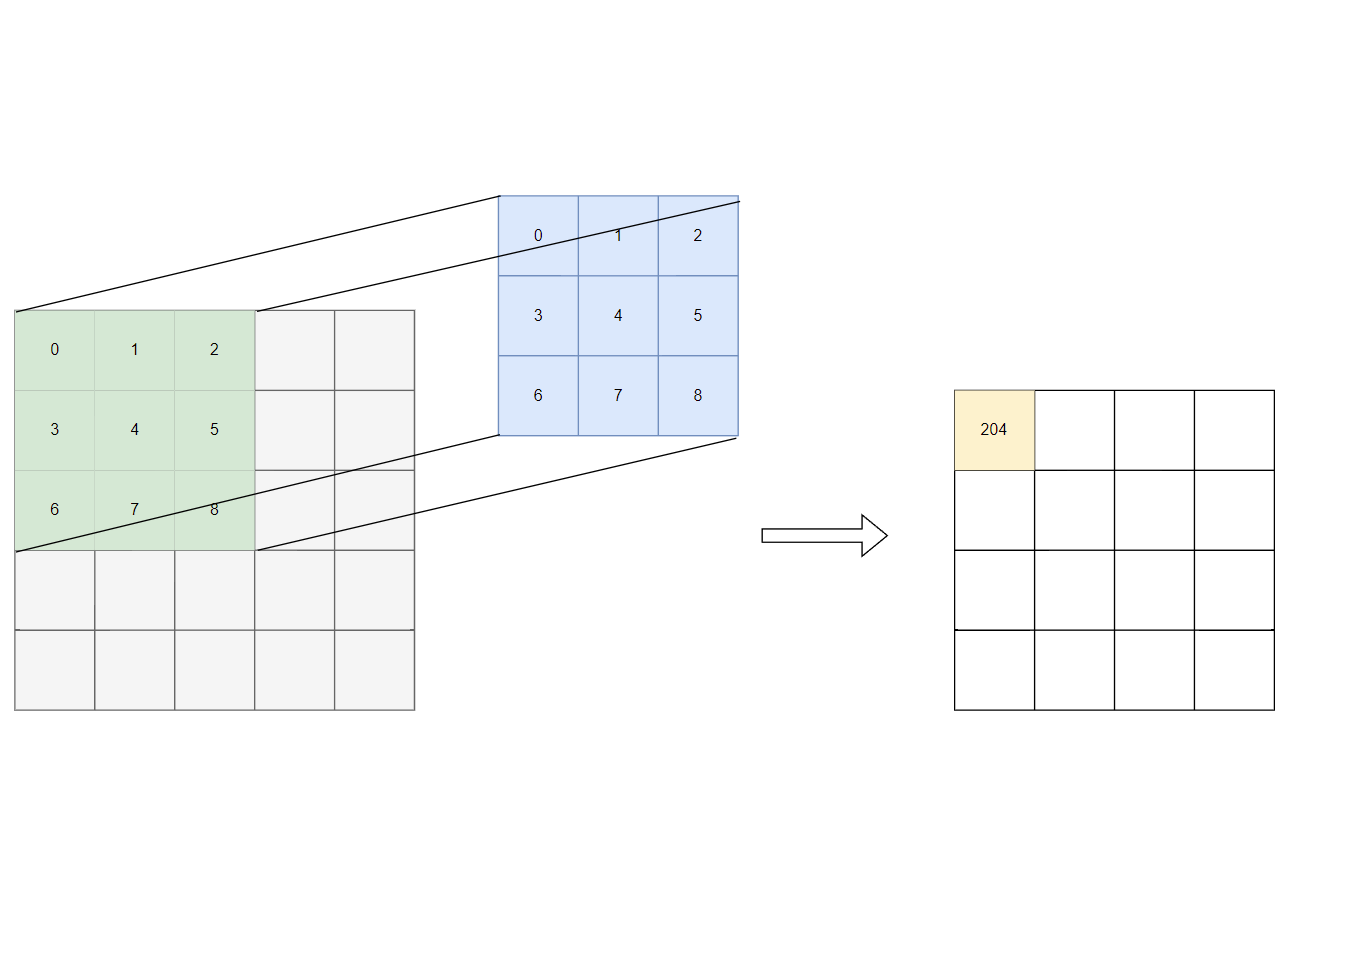
\includegraphics[width=250pt]{conv.png}
        \caption{无填充、步幅为1的卷积操作}
        \label{img_conv}
    \end{minipage}
    \hfill%分栏的意思吧
    \begin{minipage}[t]{0.5\linewidth}
        \centering
        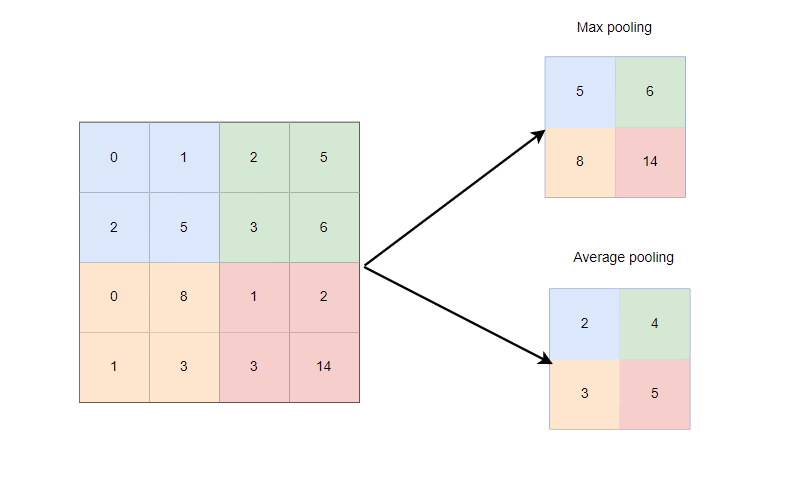
\includegraphics[width=250pt]{pooling.png}
        \caption{最大池化和平均池化操作}
        \label{img_pooling}
    \end{minipage}
\end{figure}

% \begin{figure*}
%     \centering
%     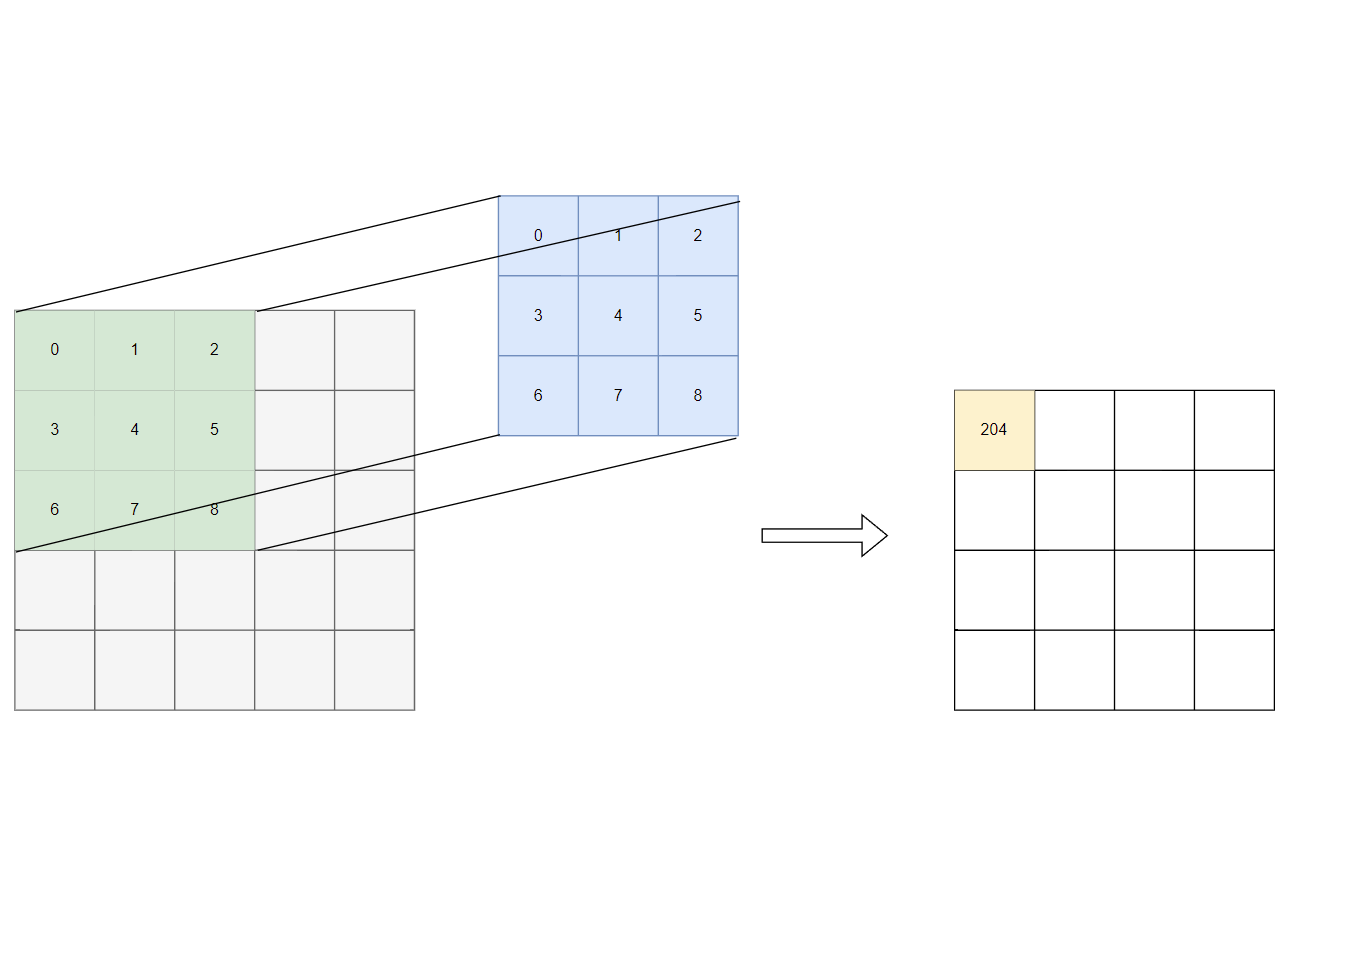
\includegraphics[width=200pt]{conv.png}
%     \caption{卷积} \label{conv}
% \end{figure*}
\subsection{池化}
池化操作对输入进行下采样,降低输入的尺寸大小,进行特征的过滤和提取。池化层可以降低卷积层对于位置的敏感性,常用的池化操作有最大池化和平均池化。最大池化操作计算窗口区域的最大值,平均池化操作计算窗口区域内的平均值。最大池化和平均池化都降低图片分辨率,但最大池化保留池化窗口中的最大值,即图片的最突出特征,通常效果更好一些。

在图像处理中,池化层一般作用于卷积层之后,通过对图片输入进行填充,使得卷积层不改变输入大小。然后通过池化层进行下采样操作,提取数据特征。池化层不需要学习,通常池化层采用$2\times 2$大小,步幅为2,对图像进行2倍下采样操作,使得输入的高度和宽度减半。
如\cref{img_pooling}所示,分别为最大池化和平均池化操作。





\section{上采样}
上采样,即对图像进行放大,提升图像的分辨率。上采样的方法主要有双线性插值(bilinear)、转置卷积(transposed convolution)、UnSampling和Unpooling\textsuperscript{\cite{zeiler2014visualizing, noh2015learning}}等。在对图片进行下采样提取特征的过程中,会使图片变小。而对于图像分割问题,我们希望输出图像与输入图像大小相同,以得到对于输入图像的分割图。这一目标需要通过上采样操作来实现,上采样可以放大图像,使图像逐步恢复到原图大小。

\subsection{双线性插值}
双线性插值作用于具有两个变量的函数,分别在两个方向上各进行一次线性差值。假设已知$\mbox{函数f在}Q_{11}(x_1,y_1), Q_{21}(x_2,y_1), Q_{12}(x_1,y_2), Q_{22}(x_2,y_2)$处的值,要求得$\mbox{函数f在}P(x,y)$处的值,如\cref{bilinear}。首先在x方向上进行一次线性差值:
\begin{equation}
    \begin{split}
        f(P_1)\approx \frac{x_2-x}{x_2-x_1}f(Q_{11})+\frac{x-x_1}{x_2-x_1}f(Q_{21})\\
        f(P_2)\approx \frac{x_2-x}{x_2-x_1}f(Q_{12})+\frac{x-x_1}{x_2-x_1}f(Q_{22})
    \end{split}
\end{equation}

在x方向得到的两个点$P_1(x,y_1), P_2(x,y_2)$处的值,对这两个点在y方向上在进行一次差值,得到点$P(x,y)$处的值。
\begin{equation}
    f(P)=\frac{y_2-y}{y_2-y_1}f(P_2)+\frac{y-y_1}{y_2-y_1}f(P_1)
\end{equation}
\begin{figure*}[htbp]
    \centering
    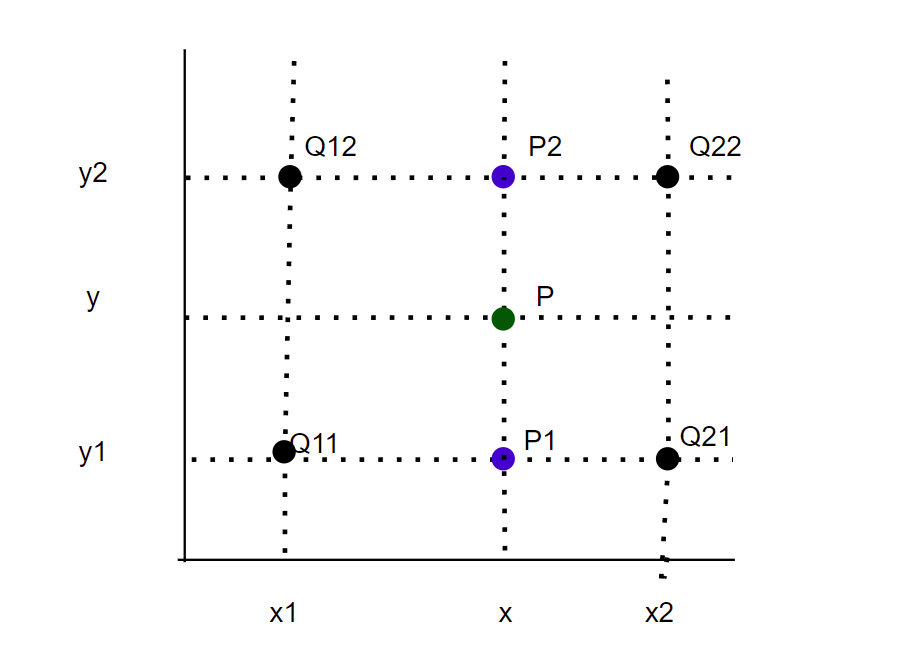
\includegraphics[width=200pt]{bilinear.png}
    \caption{双线性插值}
    \label{bilinear}
\end{figure*}

在计算机视觉和图像处理中,双线性差值利用周围四个特征点的值来求得一个新的像素点信息,在进行图片放大时可以接近原图片的视觉效果,减少图片失真。



\subsection{转置卷积}
卷积和池化操作通常会减少输入大小,而对于图像分割,需要输出大小与输入大小相同,可以看作像素级的分类问题。转置卷积进行上采样增大输入大小,把提取的高维特征进行解码。转置卷积通过卷积核对来自输入的元素进行广播,逆转下采样导致的空间尺寸变小。\cref{transconv}为将$2\times 2$转置卷积核作用于$2\times 2$的输入矩阵,步幅为2时的输出:
\begin{figure}[htbp]
    \begin{minipage}[t]{0.5\linewidth}  %并排插图时,线宽很重要,自己慢慢试,俩张图就不要超过0.5,三张图不要超过0.33之类的,自己看着办  
        \centering
        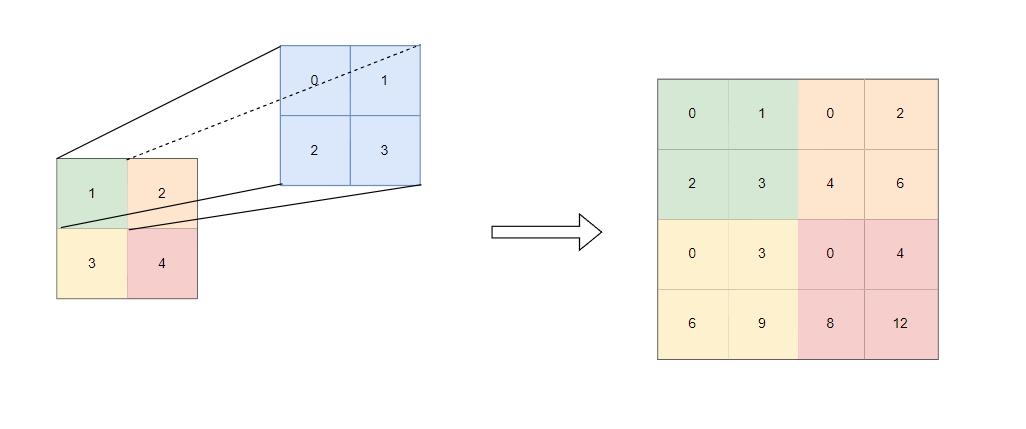
\includegraphics[width=250pt]{transconv.png}
        \caption{$2\times 2$,步幅为2的转置卷积操作}
        \label{transconv}
    \end{minipage}
    \hfill%分栏的意思吧
    \begin{minipage}[t]{0.5\linewidth}
        \centering
        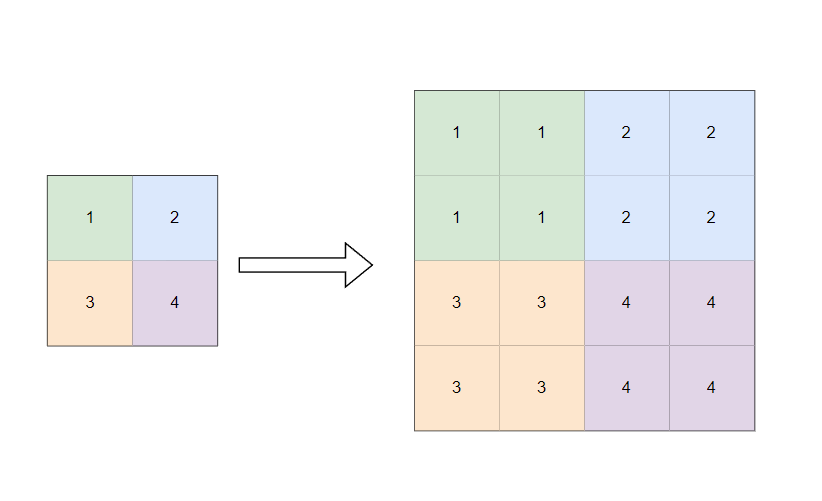
\includegraphics[width=250pt]{unsampling.png}
        \caption{UnSampling操作}
        \label{unsampling}
    \end{minipage}
\end{figure}

\subsection{UnSampling和Unpooling}
UnSampling通过将相应位置的值填充复制到一定区域内,实现对图片的放大,类似于逆平均池化层的操作,\cref{unsampling}描述了UnSampling操作。Unpooling与UnSampling操作类似,不过Unpooling会保存Maxpooling时的最大值位置信息,在Unpooling时将值填入到记录的位置信息处,其余位置补0。




\section{图像分割评估指标}
常用于评估图像语义分割效果的评估指标有像素精度(pixel accuracy, PA),平均像素精度(mean pixel accuracy, MPA),Jaccard相似系数,Dice相似系数等。
\subsection{像素精度}
像素精度计算被正确预测的像素点数占图像总像素点数的比例,假设有$k+1$个类别,$P_{ij}$表示类别为i的像素点被预测为类别j的数目。像素精度定义如下:
\begin{equation}
    PA=\frac{\sum\limits_{i=0}^{k}P_{ii}}{\sum\limits_{i=0}^{k}\sum\limits_{i=0}^{k}P_{ij}}
\end{equation}

\subsection{平均像素精度}
平均像素精度与像素精度的区别在于,平均像素精度计算每一类别被正确预测的像素点数占该类别像素的总数的比例,并对每一类别的被正确预测的比例求和后再求平均值。

\begin{equation}
    MPA=\frac{1}{k+1}\sum\limits_{i=0}^k\frac{P_{ii}}{\sum\limits^k_{j=0}P_{ij}}
\end{equation}

\subsection{Jaccard相似系数}
Jaccard相似系数用于比较样本之间的相似性,定义为集合X和集合Y交集的大小与集合X与集合Y并集大小的比值:
\begin{equation}
    Jaccard(X, Y)=\frac{|X\cap Y|}{|X \cup Y|}=\frac{|X\cap Y|}{|X|+|Y|-|X\cap Y|}
\end{equation}
使用\cref{confusion_matrix}\textsuperscript{\cite{周志华machine}}分类结果混淆矩阵来表示Jaccard相似系数:

\begin{equation}
    Jaccard=\frac{TP}{FP+TP+FN}
\end{equation}


\subsection{Dice相似系数}
Dice相似系数,是一种集合相似度度量指标,用于计算两个样本的相似度,Dice相似系数的取值范围为[0,1]。Dice相似系数的取值越高,代表两个样本的相似度越高。X与Y的Dice相似系数定义如下:
\begin{equation}
    Dice(X, Y)=\frac{2|X\cap Y|}{|X|+|Y|}
\end{equation}

使用\cref{confusion_matrix}\textsuperscript{\cite{周志华machine}}分类结果混淆矩阵来表示Dice相似系数:

\begin{equation}
    Dice=\frac{2TP}{FP+2TP+FN}
\end{equation}




\begin{table}[htbp] %表格位置
    \setlength{\abovecaptionskip}{0cm}
    \setlength{\belowcaptionskip}{0.2cm}
    \centering
    \caption{分类结果混淆矩阵}
    \label{confusion_matrix}
    \begin{tabular}{c|c|c}
        \hline
        \diagbox{真实情况}{预测结果} & 正例         & 反例         \\
        \hline
        正例                         & TP(真正例) & FN(假反例) \\
        \hline
        反例                         & FP(假正例) & TN(真反例) \\
        \hline
    \end{tabular}
\end{table}









\section{损失函数}
在深度学习模型中,我们需要有一个函数来评估模型的优劣程度,这被称为损失函数。损失函数是评估模型网络的性能指标,我们的目标是最小化损失函数来学习模型参数的最优解。在深度学习中,常用的损失函数有平方损失函数(MSE),交叉熵损失函数(CrossEntropy)损失函数,合页损失函数(Hinge Loss)等。在图像分割领域中,常用CrossEntropy loss与Dice loss来设计损失函数。
\subsection{MSE}
平方损失函数(Mean Squared Error, MSE)计算预测值$\hat{y_i}$与真实值$y_i$的接近程度,常用于回归模型。其定义如下:
\begin{equation}
    MSE=\frac{1}{2n}\sum_{i=1}^n(y_i-\hat{y_i})^2
\end{equation}
\subsection{Dice Loss}
Dice loss在V-Net\textsuperscript{\cite{milletari2016v}}模型提出,与Dice相似系数相关,Dice相似系数评估了两个样本的相似度,而Dice loss评估了两个样本的差异。
Dice Loss定义如下,其值越大,代表X与Y的差异程度越高。
\begin{equation}
    DiceLoss(X, Y)=1-\frac{2|X\cap Y|}{|X|+|Y|}
\end{equation}
% \begin{itemize}[leftmargin=50pt, listparindent=10pt ]
%     \item Dice相似系数\\

%     \item Dice Loss\\
%           Dice Loss定义如下,其值越大,代表X与Y的差异程度越高。
%           \begin{equation}
%               DiceLoss(X, Y)=1-\frac{2|X\cap Y|}{|X|+|Y|}
%           \end{equation}
% \end{itemize}


\subsection{CrossEntropy}
% CrossEntropy用于量化两个概率分布之间的差异,假设真实概率分布为P,预测概率分布为Q,损失函数定义如下:
% \begin{equation}
%     H(P,Q)=-\sum_xP(x)logQ(x)
% \end{equation}
% \par
% $P(x)$是真实概率分布,在分类问题中通常用长度为x的独热编码向量来表示x个类别,对应类别的值为1,其余为0,而图像分割问题可以看作每个像素的分类问题。$-logQ(X)$取得在相应的真实类别预测概率,对预测概率越大时,这一项取值越小,表明预测的结果越准确。

CrossEntropy用于量化两个概率分布之间的差异,假设样本小标索引为$n=1,...,N$,真实概率分布为$y$,预测概率分布为$\hat{y}$,损失函数定义如下:
\begin{equation}
    C=-\frac{1}{N}\sum_{i=1}^{N}[y_n ln \hat{y_n}+(1-y_n)ln(1-\hat{y_n})]
\end{equation}
\par
$y_n$是真实概率分布,在分类问题中通常用长度为x的独热编码向量来表示x个类别,对应类别的值为1,其余为0,而图像分割问题可以看作每个像素的分类问题。$\hat{y_n}$取得在相应的真实类别预测概率,在损失函数前添加了负号,即$-ln \hat{y_n}$,对预测概率越大时,这一项取值越小,表明预测的结果越准确。同时由于预测的概率为$[0,1]$之间的实数,所以这一项不小于0。








\section{优化算法}
优化算法的作用是对模型的参数进行调整,优化算法试图
通过对参数的调整以找到一组合适的参数,使得模型损失可以达到全局最优。常用的优化算法有梯度下降法、AdaGrad算法、RMSprop算法和AdaDelta算法等\textsuperscript{\cite{zhang2021dive, ruder2016overview,nielsen2015neural}}。

\subsection{梯度下降法}
假设损失函数为均方损失函数$C(w,b)=\frac{1}{2n}\sum_x||y(x)-a||^2$,其中w为模型的权重,b为偏置,y(x)为输入为x时的预测值,a为对应的真实值。梯度下降的目标是求得合适的w、b参数,使得预测值接近于真实值,即$C(w,b)\approx 0$。

假设损失函数C的值取决于变量$v_1, v_2$,给予$v_1, v_2$一定的变化量,由微积分的知识,则损失函数C的变化量为:
\begin{equation}
    \Delta C \approx \frac{\partial C}{\partial v_1}\Delta v_1 + \frac{\partial C}{\partial v_2}\Delta v_2
\end{equation}

$\Delta v=(\Delta v_1,\Delta v_2)$为v的改变量,$\nabla C=(\frac{\partial C}{\partial v_1} , \frac{\partial C}{\partial v_2})^T$为函数梯度方向,梯度方向描述了函数变化量最快的方向。则$\Delta C=\Delta v \nabla C$。梯度下降的目标是使得均方损失C最小,C为一个不小于0的数,因此需要$\Delta C \leq 0$。
令$\Delta v=- \eta \nabla C$,$\eta$为一个很小的正数,则有:
\begin{equation}
    \begin{aligned}
        \Delta C \approx \Delta v \nabla C=-\eta ||\nabla C||^2 \\
        v=v-\eta \nabla C
    \end{aligned}
\end{equation}

与此类似,对应于均方损失函数中的每一个参数w、b,分别求其关于C的梯度,其中$\eta$表示学习率,然后在负梯度方向上更新参数,目的使损失函数不断降低:
\begin{equation}
    \begin{aligned}
        w_k=w_k-\eta \frac{\partial C}{\partial w_k} \\
        b_l=b_l-\eta \frac{\partial C}{\partial b_l}
    \end{aligned}
\end{equation}

\subsection{AdaGard}
梯度下降算法对所有的参数使用相同的学习率来更新参数,AdaGard算法则对不同的参数使用了不同的学习率,使得学习率适应参数。对不经常更新的参数使用较大的学习率,对经常更新的参数使用较小的学习率。AdaGard累积了历史梯度信息,来对当前参数进行更新。AdaGard参数更新规则如下:
\begin{equation}
    \begin{aligned}
        G_{t,i}=\sum_{t=1}^{t}g^2_{t,i} \\
        \theta_{t+1,i}=\theta_{t,i}-\frac{\eta}{\sqrt{G_{t,i}+\epsilon}}g_{t,i}
    \end{aligned}
\end{equation}

其中,$g^2_{t,i}$表示t时刻第i维度参数梯度值的平方,$ G_{t,i}$累积了从1时刻到t时刻第i维度参数梯度值的平方,$\epsilon$是为了维持数值稳定性而添加的很小的常数,$\theta_{t,i}$表示t时刻第i维度的参数。则在t+1时刻,对$\theta_{t+1,i}$的更新学习率为$\frac{\eta}{\sqrt{G_{t,i}+\epsilon}}$,可以看到随着累积梯度值的不断增大,相应的参数的学习率不断变小。Adagard的主要优点是不需要手动调整学习率,学习率会随着梯度的累积不断更新。

\subsection{RMSprop和AdaDelta}
RMSprop和AdaDelta都使用了指数加权移动平均来对AdaGard优化算法进行调整,假设$v_{t-1}$是$t-1$时刻的指数加权移动平均值,$\theta_t$是$t$时刻的值,$t$时刻的指数加权移动平均为:
\begin{equation}
    v_t=\beta v_{t-1}+(1-\beta)\theta_t=(1-\beta)\theta_t+\sum_{i=1}^{t-1}(1-\beta)\beta^i \theta_{t-i}
\end{equation}

其中$0\leq \beta \le 1, v_0=0$。

AdaGard因为不断累积每一时刻梯度的平方,学习率会不断减小,从而导致模型收敛变慢。为了解决AdaGard算法学习率不断减小的问题,提出了RMSprop算法和AdaDelta算法。
RMSprop算法对当前时刻之前的累积梯度和当前时刻计算的梯度进行指数加权移动平均,使得学习率不致于下降的过于剧烈。


RMSProp的参数更新规则如\cref{RMSProp}所示。
\begin{equation}
    \begin{aligned}
        E[g^2]_t=\gamma E[g^2]_{t-1}+(1-\gamma)g^2_{t} \\
        \theta_{t+1}=\theta_{t}-\frac{\eta}{\sqrt{E[g^2]_t+\epsilon}}g_{t}
    \end{aligned}
    \label{RMSProp}
\end{equation}

AdaDelta\textsuperscript{\cite{zeiler2012adadelta}}与RMSprop对AdaGard的改进思想一样,在RMSprop基础上,AdaDelta还维护了参数变化量的指数平均。除此之外,AdaDelta不需要设置学习率,因为学习率从参数更新规则中移除了。

\begin{equation}
    \begin{aligned}
        E[g^2]_t=\gamma E[g^2]_{t-1}+(1-\gamma)g^2_{t}                                               \\
        E[{\Delta} {\theta^2}]_t=\gamma E[{\Delta} {\theta^2}]_{t-1}+(1-\gamma){\Delta} {\theta_t^2} \\
        \Delta \theta_t=-\frac{\sqrt{E[\theta^2]_{t-1}+\epsilon}}{\sqrt{E[g^2]_t+\epsilon}}g_{t}     \\
        \theta_{t+1}=\theta_{t}+\Delta \theta_t
    \end{aligned}
    \label{AdaDelta}
\end{equation}

\section{U-net模型结构}


U-net由Olaf Ronneberger等\textsuperscript{\cite{ronneberger2015u}}在2015年提出,是一种全卷积神经网络,基于FCN改进得到。其网络模型结构包括一条用于提取图像特征图的收缩路径,和一条恢复图片尺寸的扩张路径。其结构看起来像是字母U,因此称为U-net。U-net最初用于医学领域的图像分割,并且取得了当时非常好的效果。在医学图像分割任务下,可获得的标注样本数量通常面临着数量不足的问题,U-net在比较少的训练集下对医学图像分割取得了非常好的分割效果。与别的网络模型相比较,U-net所需训练样本少,对图像的分割效果好。
U-net网络模型结构如\cref{u-net}\textsuperscript{\cite{ronneberger2015u}}所示:

\begin{figure*}[htbp]
    \centering
    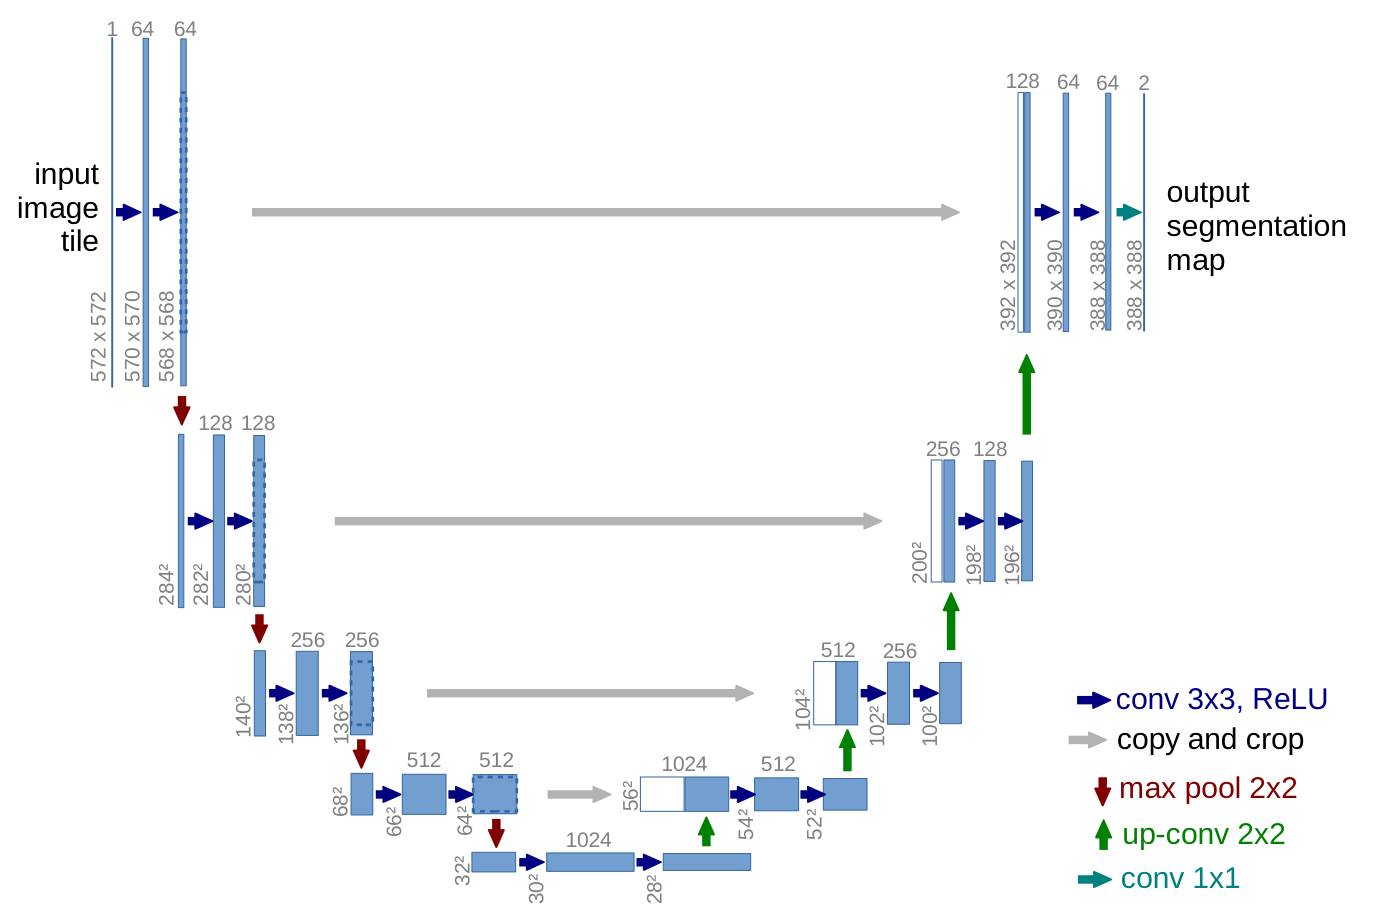
\includegraphics[width=450pt]{u-net.png}
    \caption{U-net网络模型结构}
    \label{u-net}
\end{figure*}
它由一个左侧的收缩路径和一个右侧的扩张路径组成。左侧的收缩路径是典型的卷积神经网络结构,在每一层包括两次卷积操作,每次卷积操作后用ReLU作为激活函数。采用步幅为2的最大池化层将图片尺寸减半。在每次下采样操作中将特征通道数加倍。共进行4次下采样操作,对输入图像下采样16倍。

右侧扩张路径在每一步中对特征图进行上采样,采用2*2的转置卷积核逐步加倍恢复原始图片尺寸,同时特征通道数减半。并与来自对应收缩路径层裁剪的特征图进行拼接,构成特征通道数加倍的特征图。然后分别进行两次卷积操作,每次卷积操作采用ReLU作为激活函数。对应于4次下采样操作,进行4次上采样操作,恢复到原图片大小。



\chapter{基于改进的U-net网络模型进行小样本图像分割}

\section{问题提出和解决思路}
当前,针对U-net这一经典的图像分割模型已经提出了很多改进策略。在卷积神经网络中,浅层的卷积层的感受野比较小,对于图片细节的学习感知能力比较强。深层的卷积层,因为下采样操作降低了图片的分辨率,所以感受野相对增大,可以学习到图片的整体特征。U-net使用了长连接,将来自浅层卷积层提取的特征图与深层卷积层通过上采样恢复的特征图在通道上进行拼接,使通道数加倍。Zongwei Zhou等在此基础上提出了Unet++网络\textsuperscript{\cite{zhou2018unet++}},认为直接将来自于下采样的浅层特征与上采样的深层特征进行连接会带来semantic gap。U-net仅对第四次下采样得到的特征图进行上采样操作,而U-net++则对每次下采样得到的特征图都进行了上采样操作,在U-net网络的基础上添加了更多的长连接操作,降低下采样阶段和上采样阶段得到的特征图的语义差异。U-net 3+\textsuperscript{\cite{huang2020unet}}在U-net++的基础上,进一步改进,不仅在对应的上采样阶段有来自同层次的特征图,还包括每一个下采样阶段的特征图。
何凯明等提出的ResNet\textsuperscript{\cite{he2016deep}}很好的解决了深度神经网络的训练问题,输入可以通过在残差块中添加的残差连接更快的向前传播,Zhang Zhengxin等结合ResNet和U-net提出了ResUnet\textsuperscript{\cite{zhang2018road}}。

当模型容量过大,模型过于复杂时,模型很容易出现过拟合问题\textsuperscript{\cite{goodfellow2016deep}}。由于深度神经网络强大的学习能力,在进行小样本训练时,相对于模型容量,数据特征维度偏少,因此较容易出现过拟合问题。因此,为了解决小样本图像分割这一问题,从数据和模型两方面来进行研究。首先针对训练数据不足的问题,对数据进行数据增强。更多的数据可以增加数据特征,同时也有助于模型学习数据之间的相关性。在进行小样本图像分割问题的研究时,发现模型对于边缘的效果分割不好,对细节的表现不够理想。针对这一问题,对损失函数进行设计,提高模型对于边缘分割的敏感度。同时降低模型的复杂度,因为所要研究的问题小样本图像分割基于U-net模型,在U-net模型中对模型复杂度影响最大的便是每次采样阶段进行的两次卷积操作,因此考虑对其中的两次$3\times 3$卷积操作进行改进,减少模型需要训练的参数量。同时,由于残差网络在深层神经网络训练时表现出很好的效果,本文参照ResUnet对于U-net网络的改进思路,将U-net网络每一层的两次卷积操作添加残差连接。

\section{数据增强}
数据集来源于Kaggle的Carvana Image Masking Challenge,这一数据集包括不同种类的车辆在不同背景下的照片,同一车辆在不同角度的图片以及车辆对应的分割图。选择这个数据集的原因首先是因为它的图片构成要素比较简单,没有复杂的背景信息,便于分析和比较;其次,每个图片只有一个要分割的实例。同时,不同车辆又有比较大的差异化特征。从中选择10种汽车,每种汽车5张图片,共50张图片作为训练集;同时选择200张图片作为验证集,验证对于图片的分割效果。因为对于不同的任务,不同的数据集,其有效的数剧增强策略一般是不同的。同时受限于时间和本人水平的原因,只采用了这一个数据集来进行小样本图像分割的研究。

小样本学习要面对主要问题便是可用于进行训练的数据不足,在训练神经网络模型时,我们的目标是使模型损失不断降低,尽可能得到最优解。而深度神经网络有着大量的参数,在缺乏足够的数据支撑时,很难训练网络模型求解得到比较优的参数。同时,Aharon Azulay等\textsuperscript{\cite{Azulay2019WhyDD}}指出,神经网络在最初的时候并没有那么聪明,对小的图片转换操作具有比较大的敏感性。通过对现有的数据增强,对图片应用翻转,移位,旋转,水平变换等操作,我们可以扩充数据规模,同时也有助于模型学习在进行转换前后图片中的相关性与不变形。

关于数据增强时机的选择:一种被称为线下增强(offline augmentation),即首先对所有数据进行数据增强操作后在进行模型的训练。另一种是线上增强(online augmentation)\textsuperscript{\cite{tang2020onlineaugment}},即在训练的过程中不断的在小批量上数据上进行转换。因为本论文研究的问题为小样本图像分割,面对的问题是数据量不足的情况,因此采用线下增强的方式,对数据集完成所有的数据增强转换操作后,在进行模型的训练。在常见的对图片的数据增强技术中,分析考虑可能对当前的图像分割任务可能有益的数据增强操作,并通过实验分析对比和验证他们的结果。

为了找到有助于解决图像分割问题的数据增强操作,对数据集分别进行常用的数据增强操作,并通过实验来比较其结果,验证数据增强操作的有效性。
\cref{dataaugmentation}给出了本论文中对数据集应用的数据增强操作:
\renewcommand\arraystretch{1.5} %行高为1.5倍
\begin{table}[htbp] %表格位置
    \setlength{\abovecaptionskip}{0cm}
    \setlength{\belowcaptionskip}{0.2cm}
    \centering
    \caption{对图片进行的数据增强操作}
    \label{dataaugmentation}
    \begin{tabular}{p{5cm}<{\centering}p{8cm}<{\centering}p{2.3cm}<{\centering}} %列宽和居中
        \hline
        数据增强操作             & 说明                                    \\
        \hline
        invert                   & 反转图像颜色                            \\
        hflip                    & 对图像水平翻转                          \\
        rotate                   & 对图像旋转一定角度                      \\
        affineScale              & 对图像缩放                              \\
        translateX               & 水平移位                                \\
        GaussianBlur             &
        高斯模糊                                                           \\
        ColorJitter\_hue0.5      & 随机改变图片色调,变化幅度为(-0.5, 0.5) \\
        ColorJitter\_contrast0.5 & 随机改变图片的对比度,变化幅度为(0,0.5) \\
        \hline
    \end{tabular}
\end{table}

\cref{aug_result}给出所采用的增强操作以及在验证集上通过Dice相似系数评估的结果。通过对原始数据集进行不同的数据增强操作,并与不进行数据增强进行对比,分析可以用于当前图像分割任务的数据增强操作。
不进行数据增强时,分别训练了5次和10次,进行数据增强时都训练了5次。进行一种数据增强操作时,会将现有数据集规模扩充一倍。因此将不进行数据增强,进行10次训练的作为对比,与进行数据增强的训练结果进行比较。

\begin{table}[htbp] %表格位置
    \setlength{\abovecaptionskip}{0cm}
    \setlength{\belowcaptionskip}{0.2cm}
    \centering
    \caption{数据增强操作与训练结果}
    \label{aug_result}
    \begin{tabular}{|c|c|c|}
        \hline
        数据增强操作             & 训练次数(epoch) & Dice相似系数 \\
        \hline
        不进行数据增强操作       & 5               & 0.8902       \\
        \hline
        不进行数据增强操作       & 10              & 0.9019       \\
        \hline
        invert                   & 5               & 0.5905       \\
        \hline
        hflip                    & 5               & 0.9311       \\
        \hline
        rotate                   & 5               & 0.9288       \\
        \hline
        affineScale              & 5               & 0.9301       \\
        \hline
        translateX               & 5               & 0.8976       \\
        \hline
        GaussianBlur             & 5               & 0.9036       \\
        \hline
        ColorJitter\_hue0.5      & 5               & 0.9231       \\
        \hline
        ColorJitter\_contrast0.5 & 5               & 0.9047       \\
        \hline
    \end{tabular}
\end{table}

\cref{aug_result}给出了进行的数据增强操作,训练的迭代次数以及在验证集上取得的Dice相似系数,
通过对\cref{aug_result}中结果的分析比较,对图像进行颜色反转(invert)并没有带来结果的提升,反而给训练精度带来了波动状态。
\cref{invert_rounds}为进行invert数据增强操作后,进行5次迭代训练,每次迭代在验证集上评估10 rounds时得到Dice相似系数变化情况,\cref{origin_invert}和\cref{invert_image}分别给出原始图像与反转图像的对比。
\begin{figure*}
    \centering
    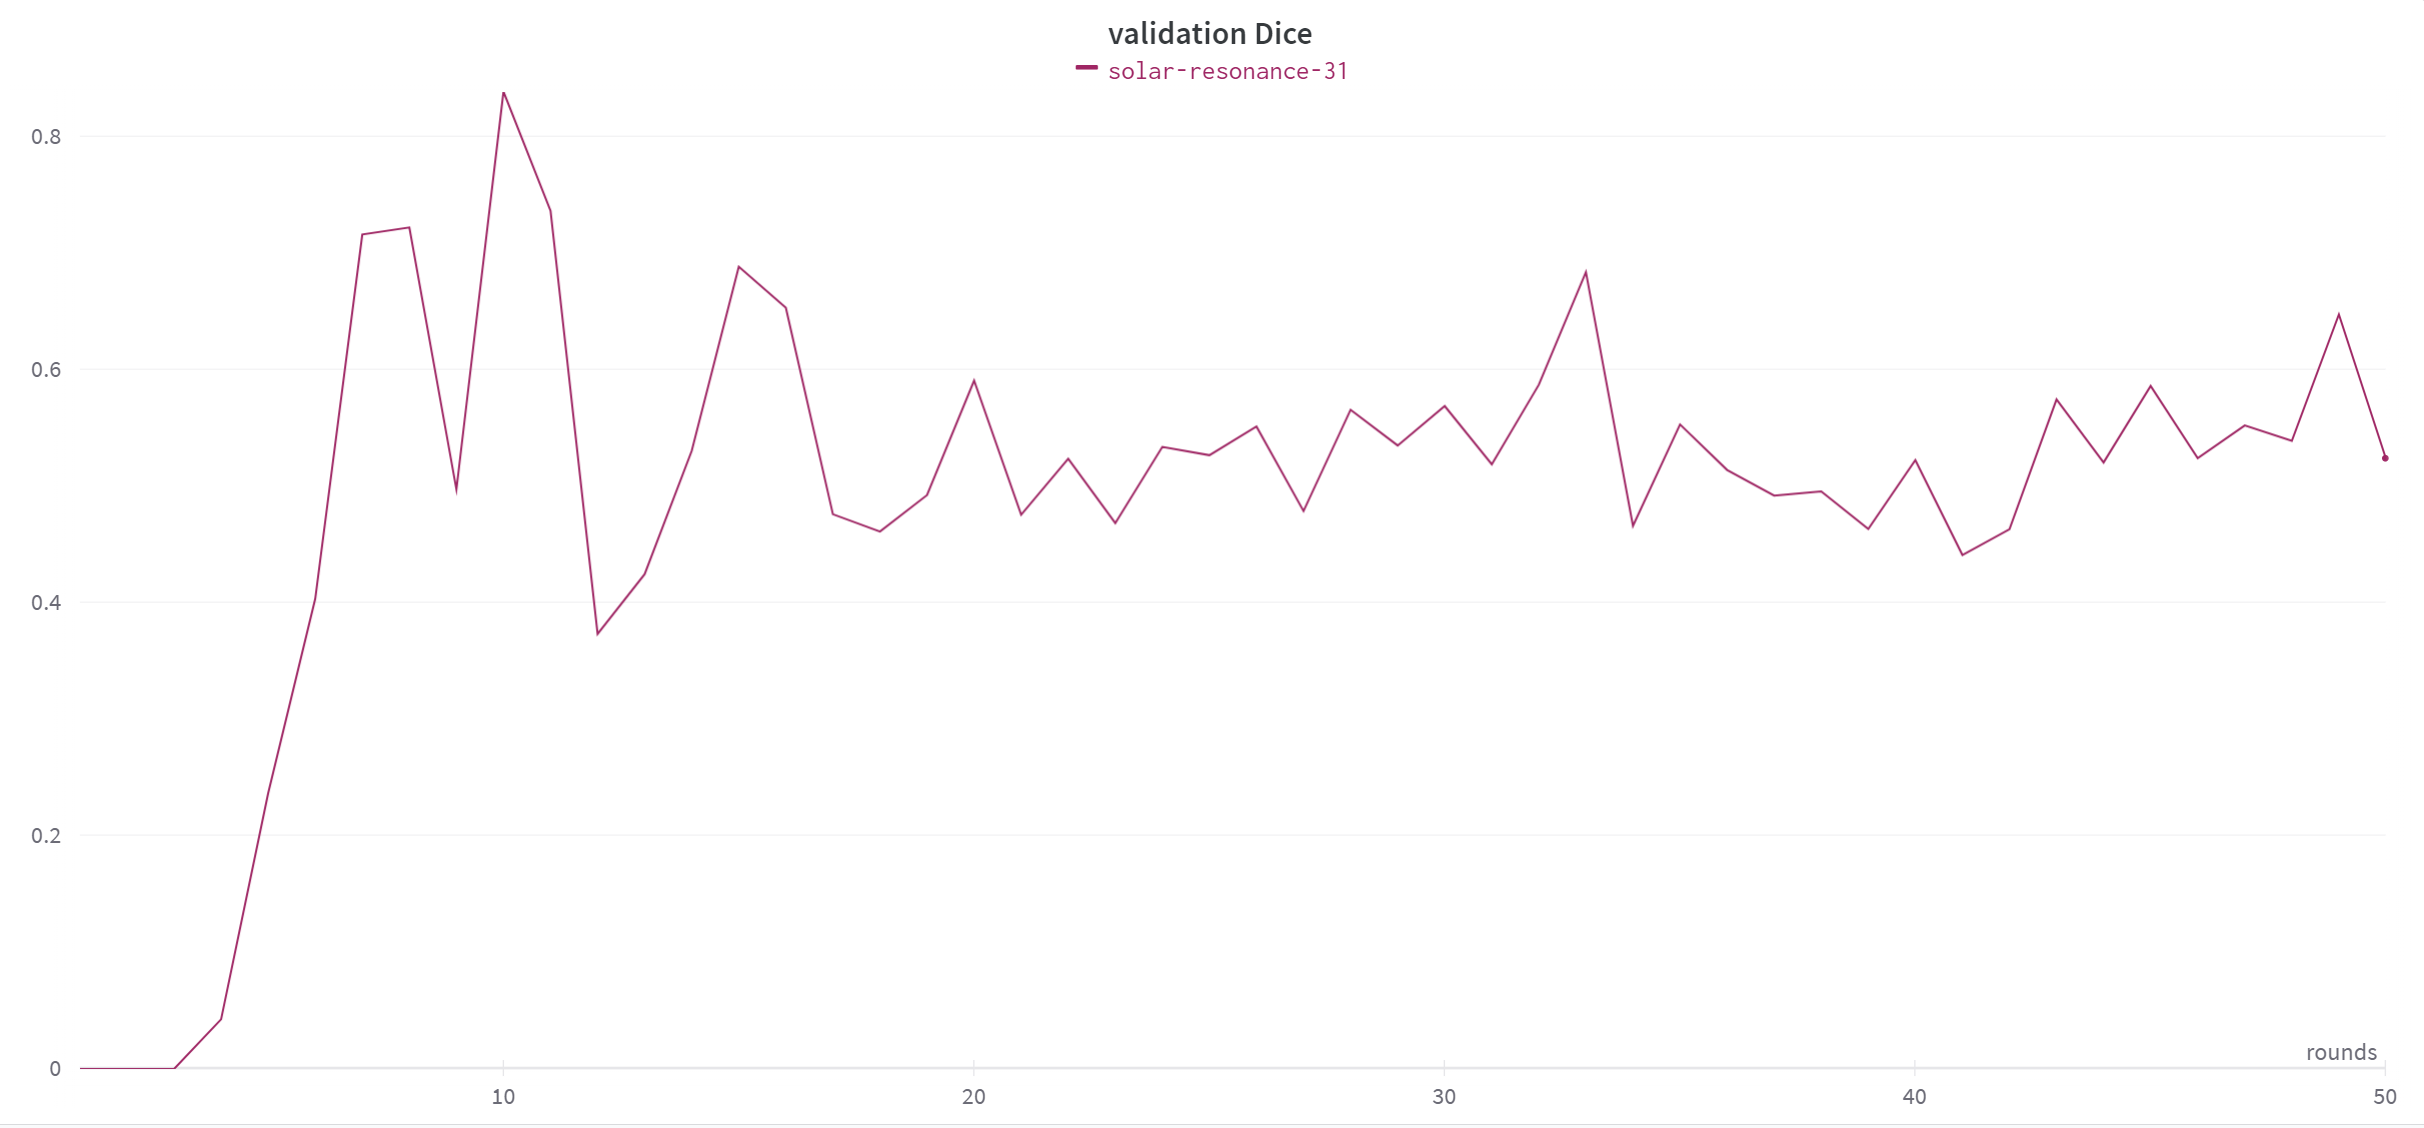
\includegraphics[width=450pt]{invert_rounds.png}
    \caption{进行invert数据增强在验证集上的Dice相似系数}
    \label{invert_rounds}
\end{figure*}

\begin{figure}[htbp]
    \begin{minipage}[t]{0.5\linewidth}  %并排插图时,线宽很重要,自己慢慢试,俩张图就不要超过0.5,三张图不要超过0.33之类的,自己看着办  
        \centering
        \includegraphics[height=4cm]{original_invert.jpg}
        \caption{原始图像}
        \label{origin_invert}
    \end{minipage}
    \hfill%分栏的意思吧
    \begin{minipage}[t]{0.5\linewidth}
        \centering
        \includegraphics[height=4cm]{invert_image.jpg}
        \caption{invert操作图像}
        \label{invert_image}
    \end{minipage}
\end{figure}

虽然从\cref{origin_invert}和\cref{invert_image}对比来看,invert操作并没有给图片形状带来太大的改变。但分析认为这与图片的计算机存储方式有关,彩色图片采用RGB三通道进行存储,对于每一个像素点,在RGB通道中分别有一个0-255的数值表示,假设某一像素点的数值为[x, y, z],invert操作为[255-x,255-y, 255-z],从数值层面分析,对图像进行反转增强操作给原始图像带来的改变比较剧烈,因此对图像特征的影响比较大。

\begin{figure*}
    \centering
    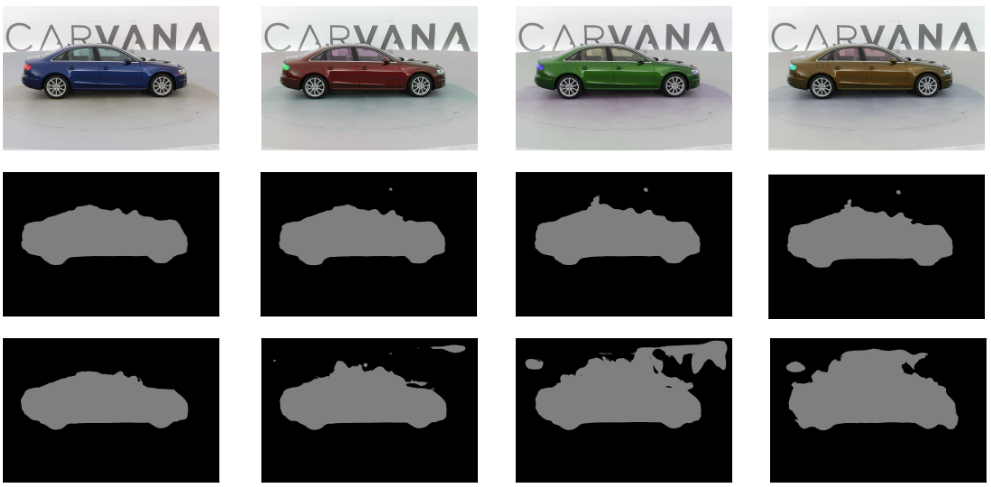
\includegraphics[width=450pt]{color_aug.png}
    \caption{对数据集进行颜色增强操作与进行颜色操作时对图像的分割情况}
    \label{color_aug}
\end{figure*}


\cref{color_aug}是对数据集进行颜色增强操作与使用原始数据集时对图像的分割情况,其中第一行左边的为原始图像,后面的图像为改变其颜色的图像,第二行为用颜色相关数据增强后得到的模型对上面图像的分割情况,第三行为不进行数据增强训练得到的模型对第一行图像的分割情况。通过对比,可以发现进行数据增强后,对四幅图像得到了差不多的分割效果;而不进行数据增强,对于四副图像的分割差异性比较大。因此,对于颜色的变换降低了网络模型对于颜色的敏感性。同时,颜色是汽车一个重要差异性指标,对于颜色的数据增强操作在当前数据集可以表现出比较好的效果。
% 5种数据增强操作(hflip、rotate、affineScale、ColorJitter\_hue0.5、ColorJitter\_contrast0.5)
同时高斯模糊和对图像进行水平移位的增强操作也没有对图像分割的结果有所提升。基于以上分析,采用5种数据增强操作(hflip、rotate、affineScale、ColorJitter\_hue0.5、ColorJitter\_contrast0.5)作为当前图像分割数据集的数据增强策略。
其中,对图片进行水平翻转和旋转的数据增强操作都提高了Dice相似系数。因为数据集中对一种汽车包括其在不同角度的16张图片,而训练数据集则只有5张图像,即五个角度的图片。对于图片的水平翻转和旋转操作补足了同一汽车在不同角度的图像,
而颜色相关数据增强则降低了网络模型对于图像颜色的敏感度,因此对于结果起到了提升作用。





% \begin{figure*}
%     \centering
%     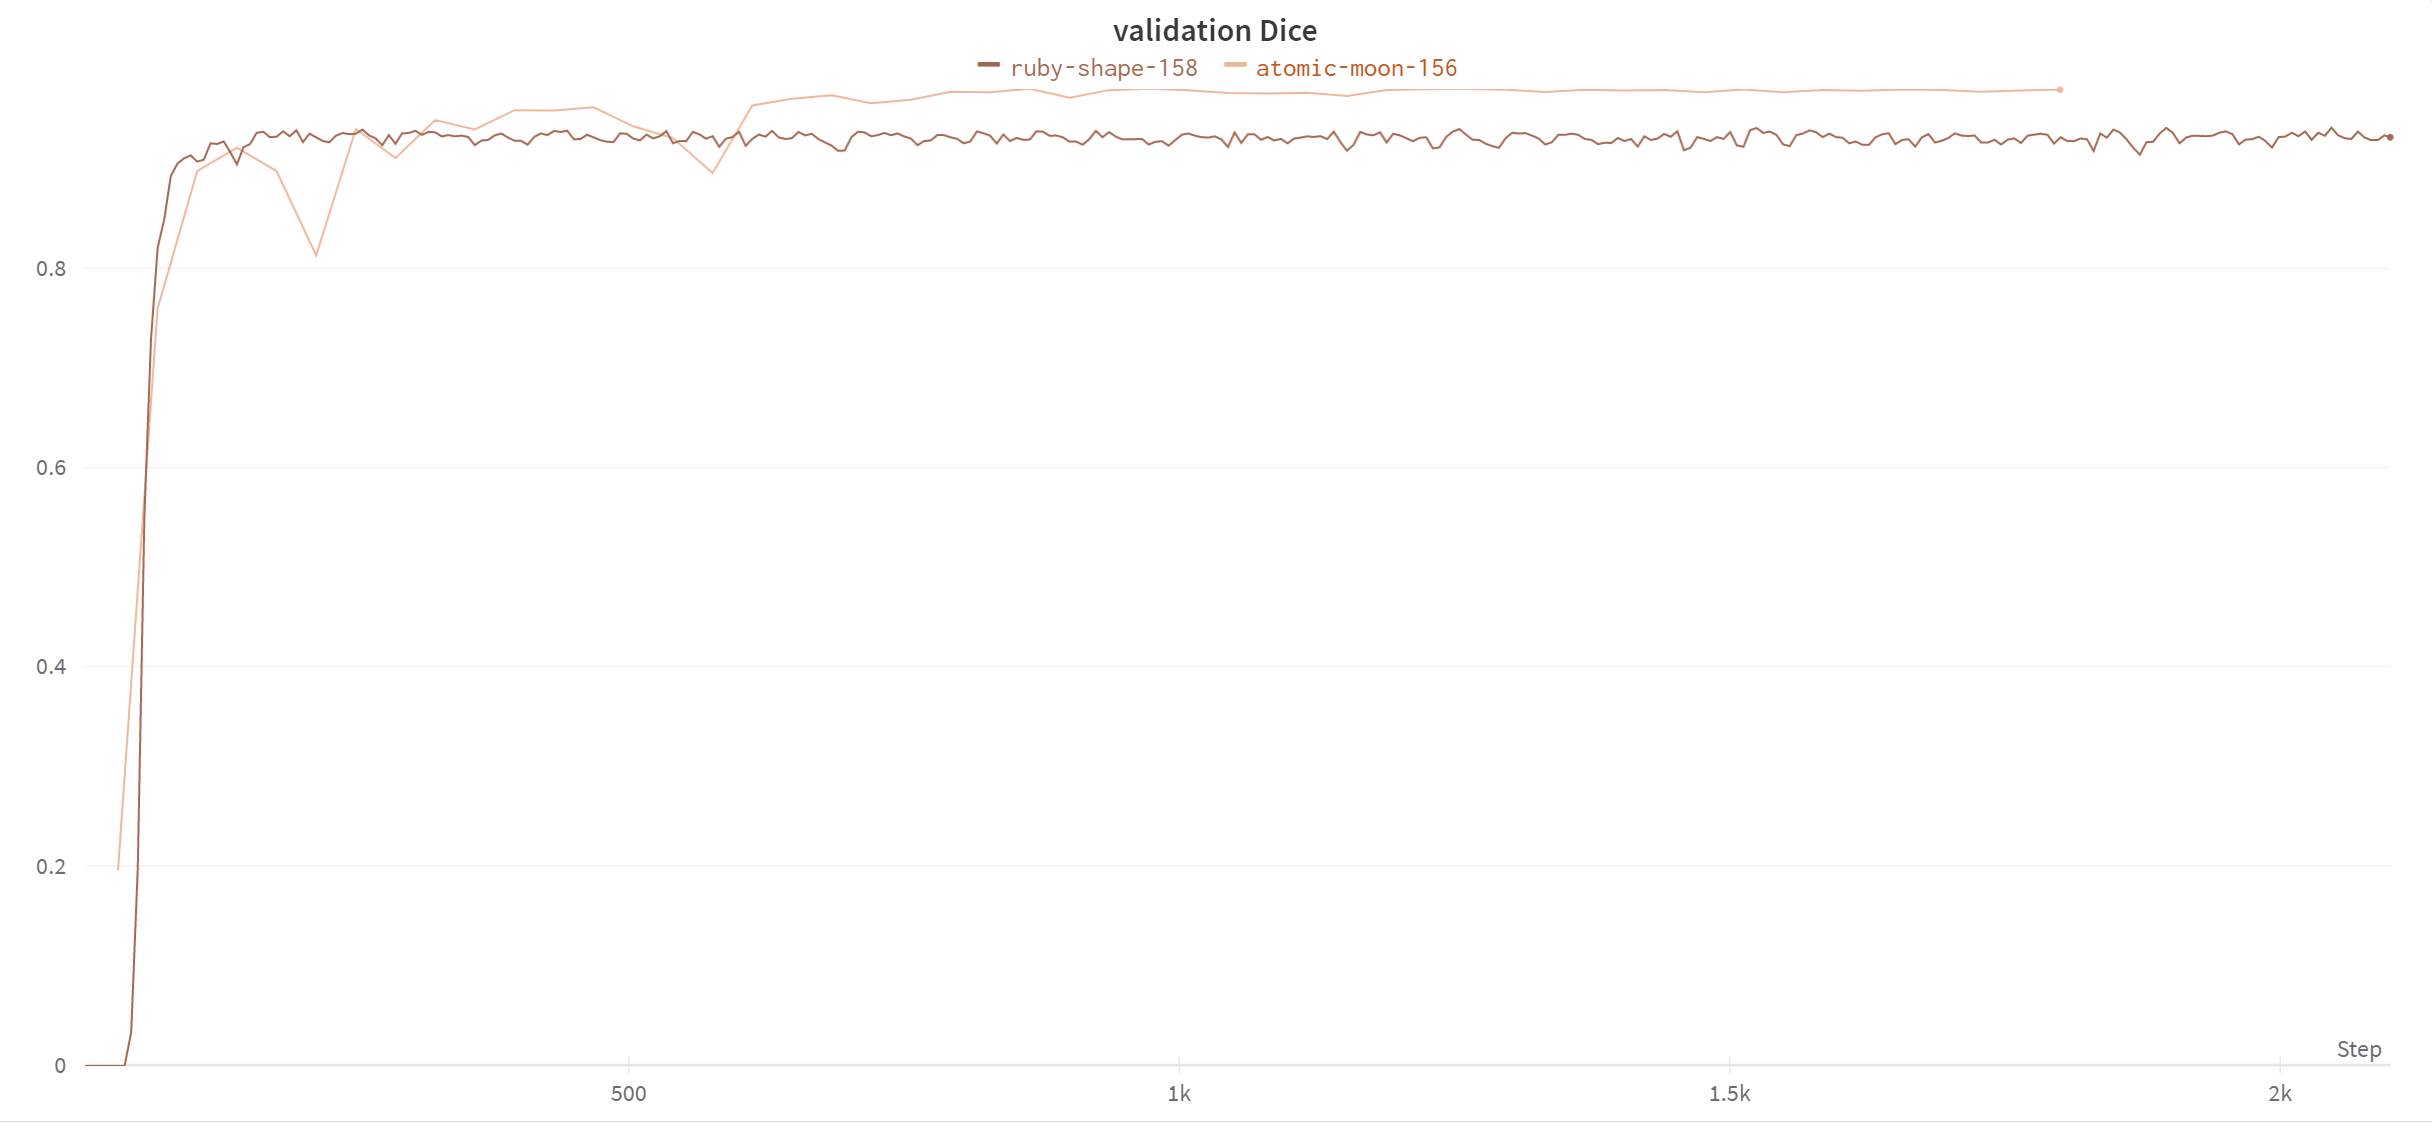
\includegraphics[width=350pt]{data_augment_result.png}
%     \caption{Dice相似系数} \label{fig6}
% \end{figure*}
% \cref{fig6}中ruby-shape-158为进行6中数据增强操作后将原始数据集扩充6倍后进行5次迭代的运行情况,atomic-moon-156为将迭代次数增加6倍,进行35次迭代的情况。对后者进行35次迭代的原因是控制两次运行所需要的总训练图像数量相同,在此基础上评估运行结果,数据增强操作对最终训练结果带来了明显的提升效果。其中,对于图片的水平翻转和旋转操作补足了同一汽车在不同角度的图像。对于颜色的变换降低了网络模型对于颜色的敏感性。





\section{损失函数设计}
在图像分割领域中,常用CrossEntropy loss与Dice loss来设计损失函数。

而在图像分割领域,经常面临的问题时是对分割的细节不准确,对边缘的分割效果不够理想,而这一问题在只有小样本用于训练时,会表现的更为明显。因此考虑在损失函数中添加一项对边缘分割效果的评估,并对边缘添加一定的权重,让神经网络对边缘的分割更加敏感。

要评估边缘分割效果,首先需要获取图像的边缘,而在数据集中,通常有的都是对实例的分割图,而没有单独的图像边缘图。基于当前采用的数据集特点,对每一个像素都是二分类问题,即这个像素要么属于背景,要么属于要分割的实例图,其中背景为0,实例为1。结合学过的位运算知识,提出一种从分割图中提取出图像边缘的方法。

如\cref{edge1}所示,中间的图为原始分割图,1表示是实例的一部分,0表示背景。将原始图像分别向上下左右平移1个像素位置,空缺的位置填补0,得到对应四个方向的图像。
\begin{figure*}[htbp]
    \centering
    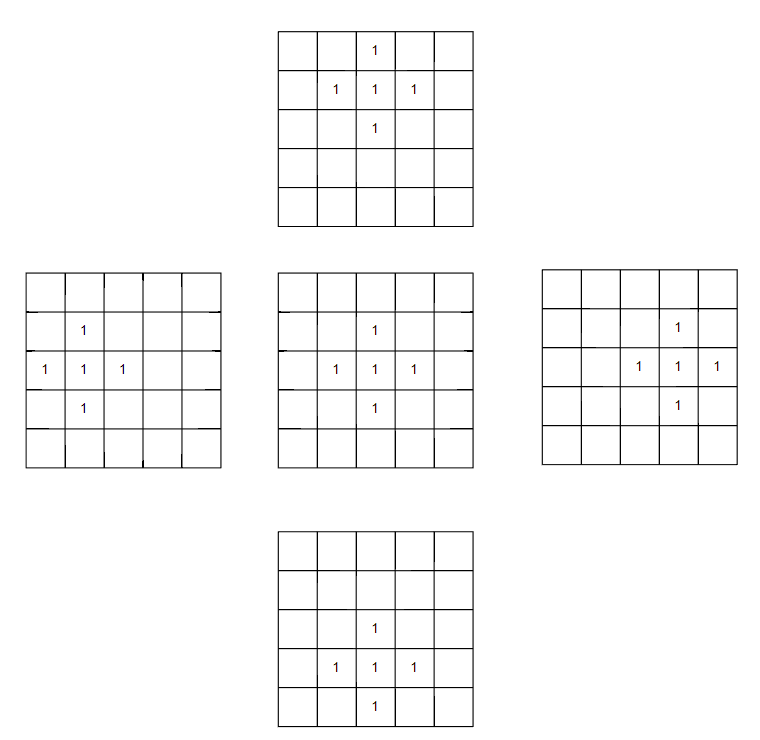
\includegraphics[width=300pt]{edge1.png}
    \caption{分割图(mask)与向四个方向平移后的图像}
    \label{edge1}
\end{figure*}

\begin{figure*}[htbp]
    \centering
    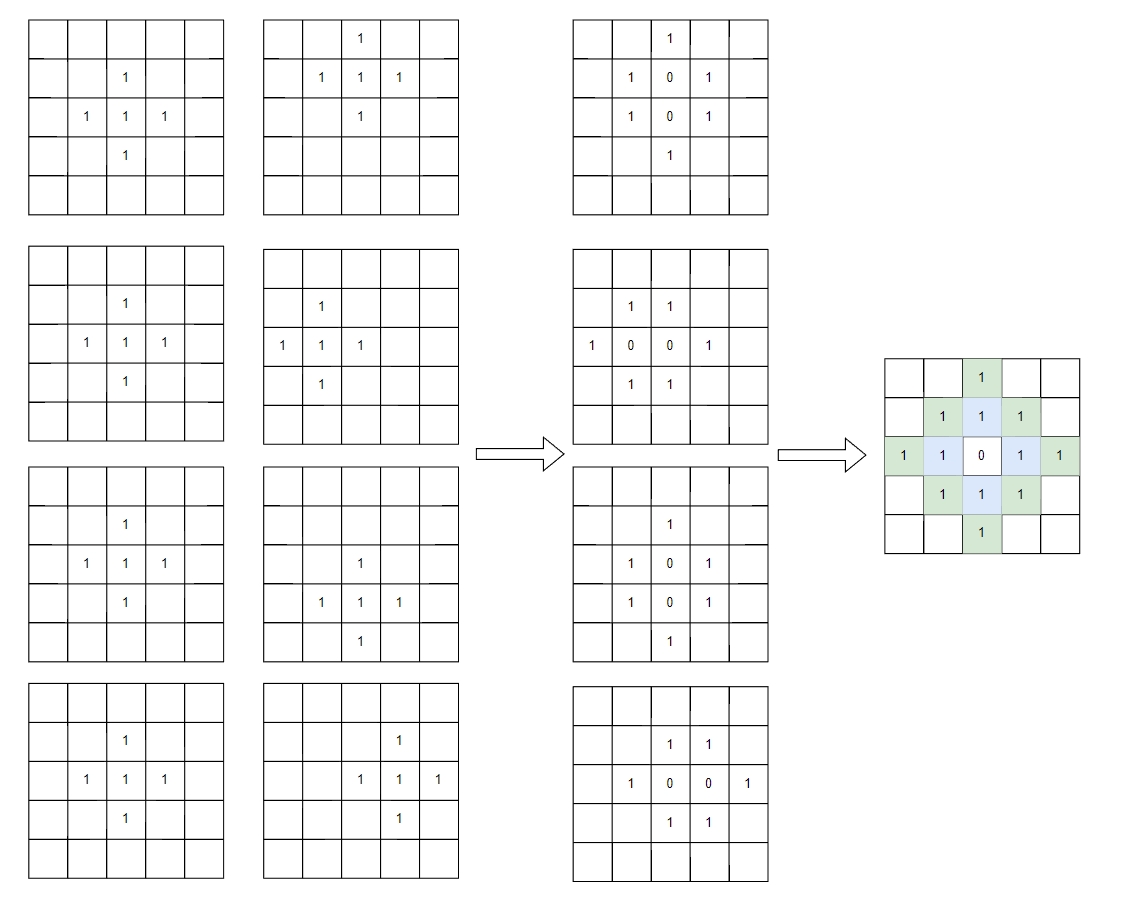
\includegraphics[width=400pt]{edge2.png}
    \caption{从mask图得到edge\_outline图}
    \label{edge2}
\end{figure*}

\begin{figure*}[htbp]
    \centering
    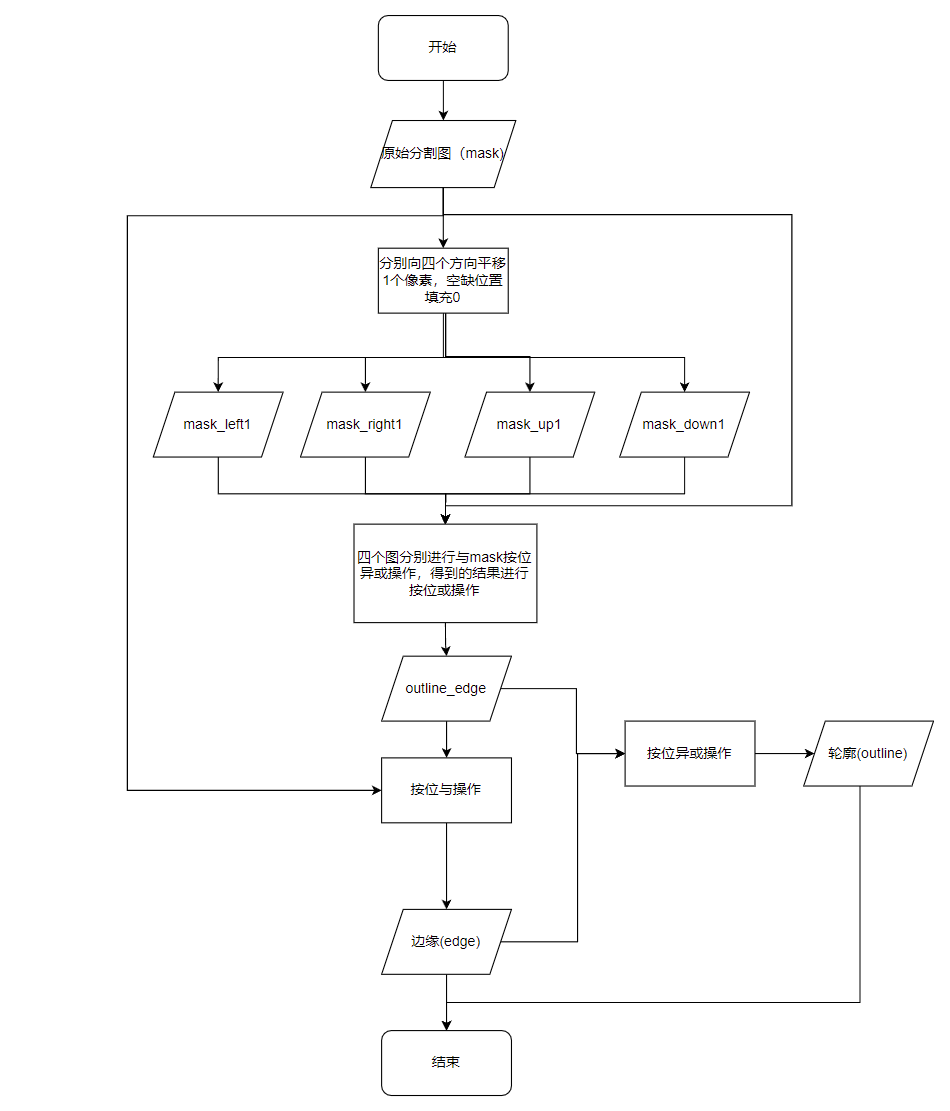
\includegraphics[width=500pt]{edge_flow.png}
    \caption{从分割图(mask)提取出边缘和轮廓的流程}
    \label{edge_flow}
\end{figure*}

\cref{edge_flow}描述了从分割图(mask)中提取出边缘的流程,流程图中edge\_outline对应\cref{edge2}中最右侧的图,将蓝色背景的称为边缘(edge),绿色背景的称为轮廓(outline)。edge\_outline既包括实例的最外面的属于实例的一个像素,也包括这一像素外的一个像素。进一步,流程图描述了如何从这个图进一步提取出边缘和轮廓的过程。提取出这两个部分后,我们便可以对其进行分别加权来设计损失函数,同时这两个部分也是对于分割图边缘分割效果影响最大的部分。然后对于其的损失函数计算方式采用如下的计算方式:
\begin{equation}
    EdgeLoss(X,Y)=\frac{|X\cap Y|}{|Y|}
\end{equation}
\par
X表示预测的概率,Y表示提取出的边缘图,这里采用与Dice Loss有些差异的计算方式,因为这一损失项只关注对边缘的分割情况。$|X\cap Y|$表示两个集合对应元素点乘,将结果相加求和。




% \begin{figure*}
%     \centering
%     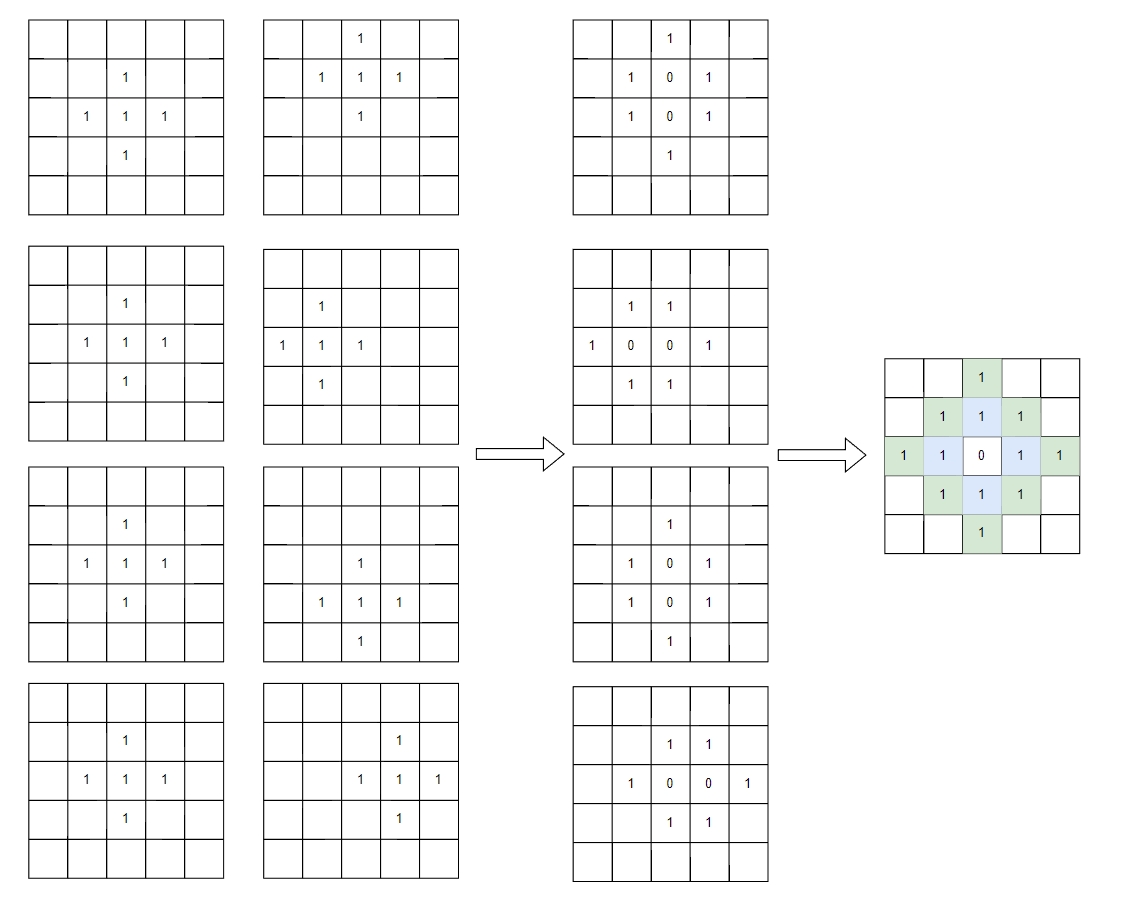
\includegraphics[width=350pt]{edge2.png}
%     \caption{从mask图得到edge_outline图}
%     \label{edge2}
% \end{figure*}



\cref{mask_edge_ans}所示,为通过上述方式提取出的边缘图:

\begin{figure}[htbp]
    \centering
    \begin{minipage}[t]{0.4\linewidth}  %并排插图时,线宽很重要,自己慢慢试,俩张图就不要超过0.5,三张图不要超过0.33之类的,自己看着办  
        \centering
        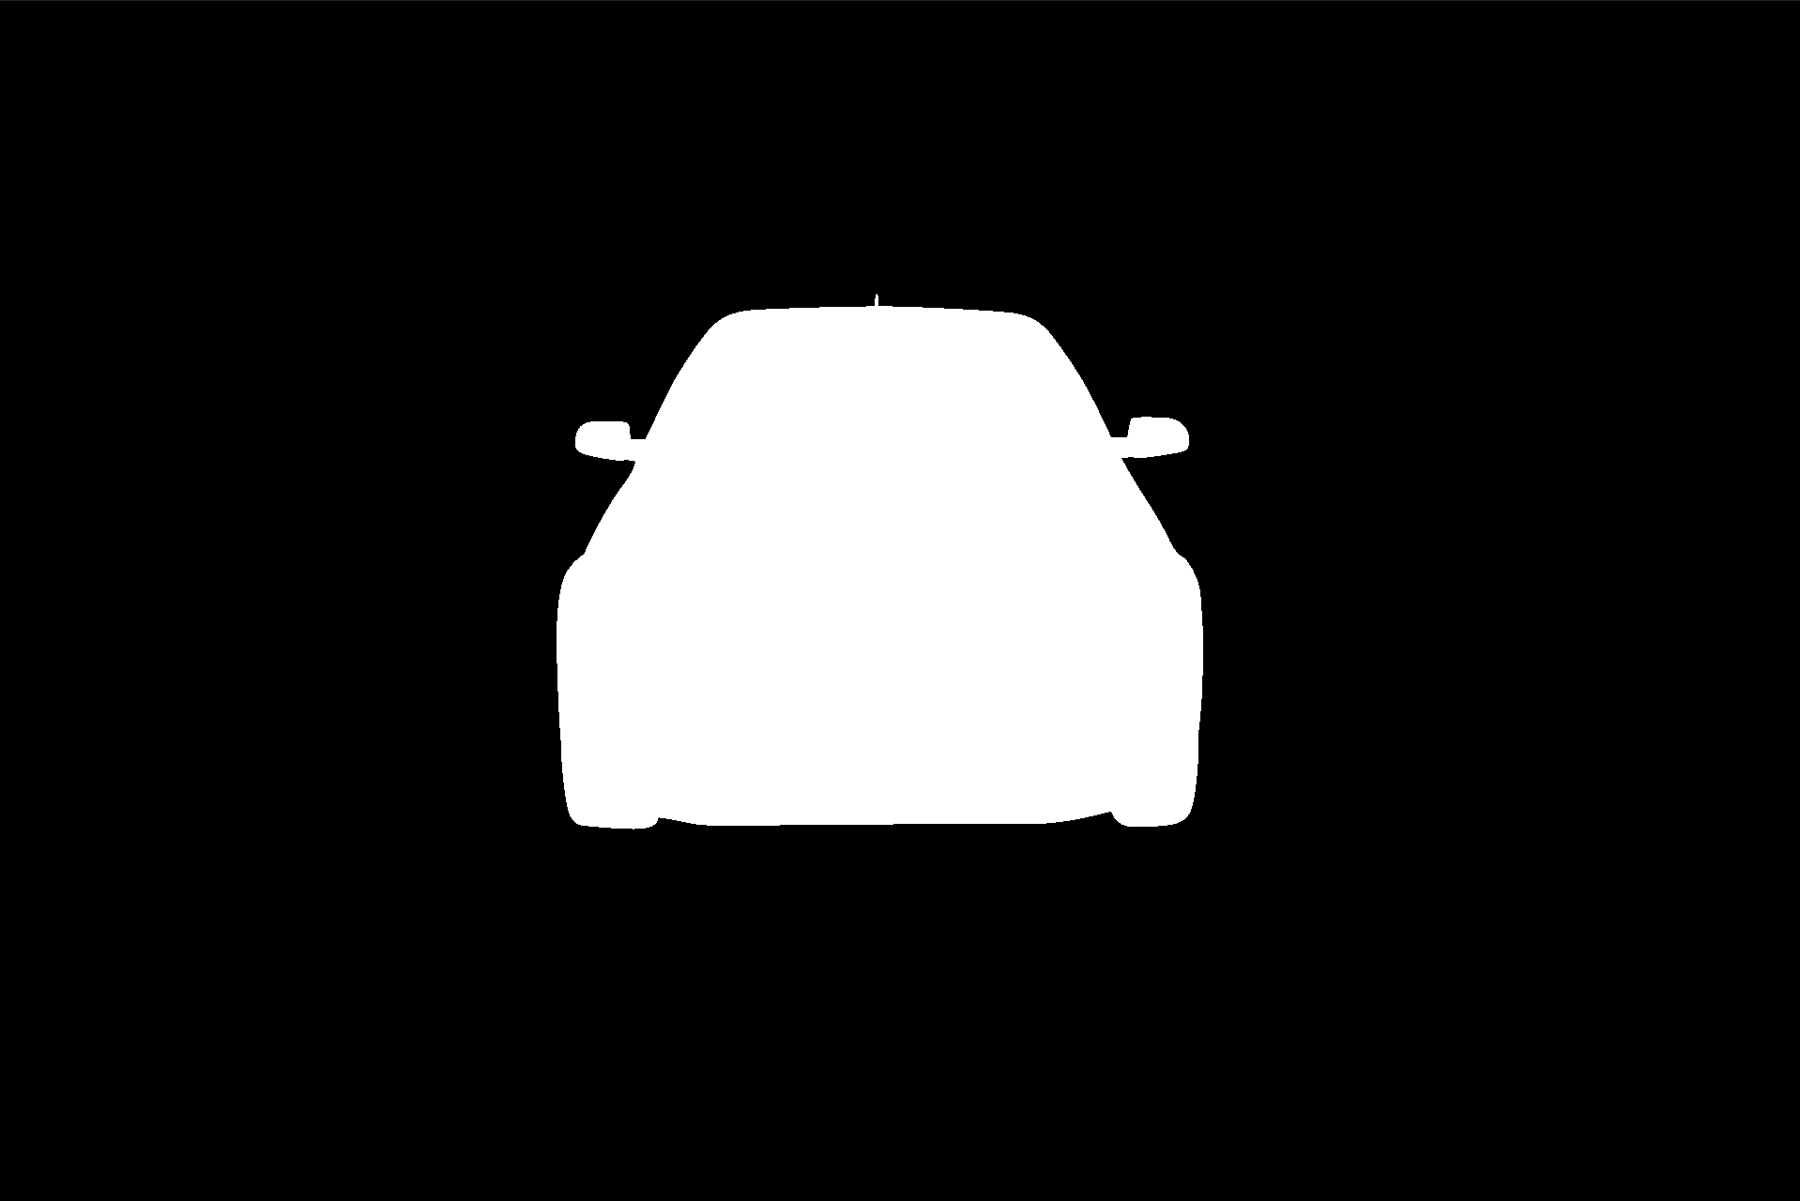
\includegraphics[height=5cm]{mask.png}
        % \caption{mask}
    \end{minipage}
    \hfill%分栏的意思吧
    \begin{minipage}[t]{0.5\linewidth}
        \centering
        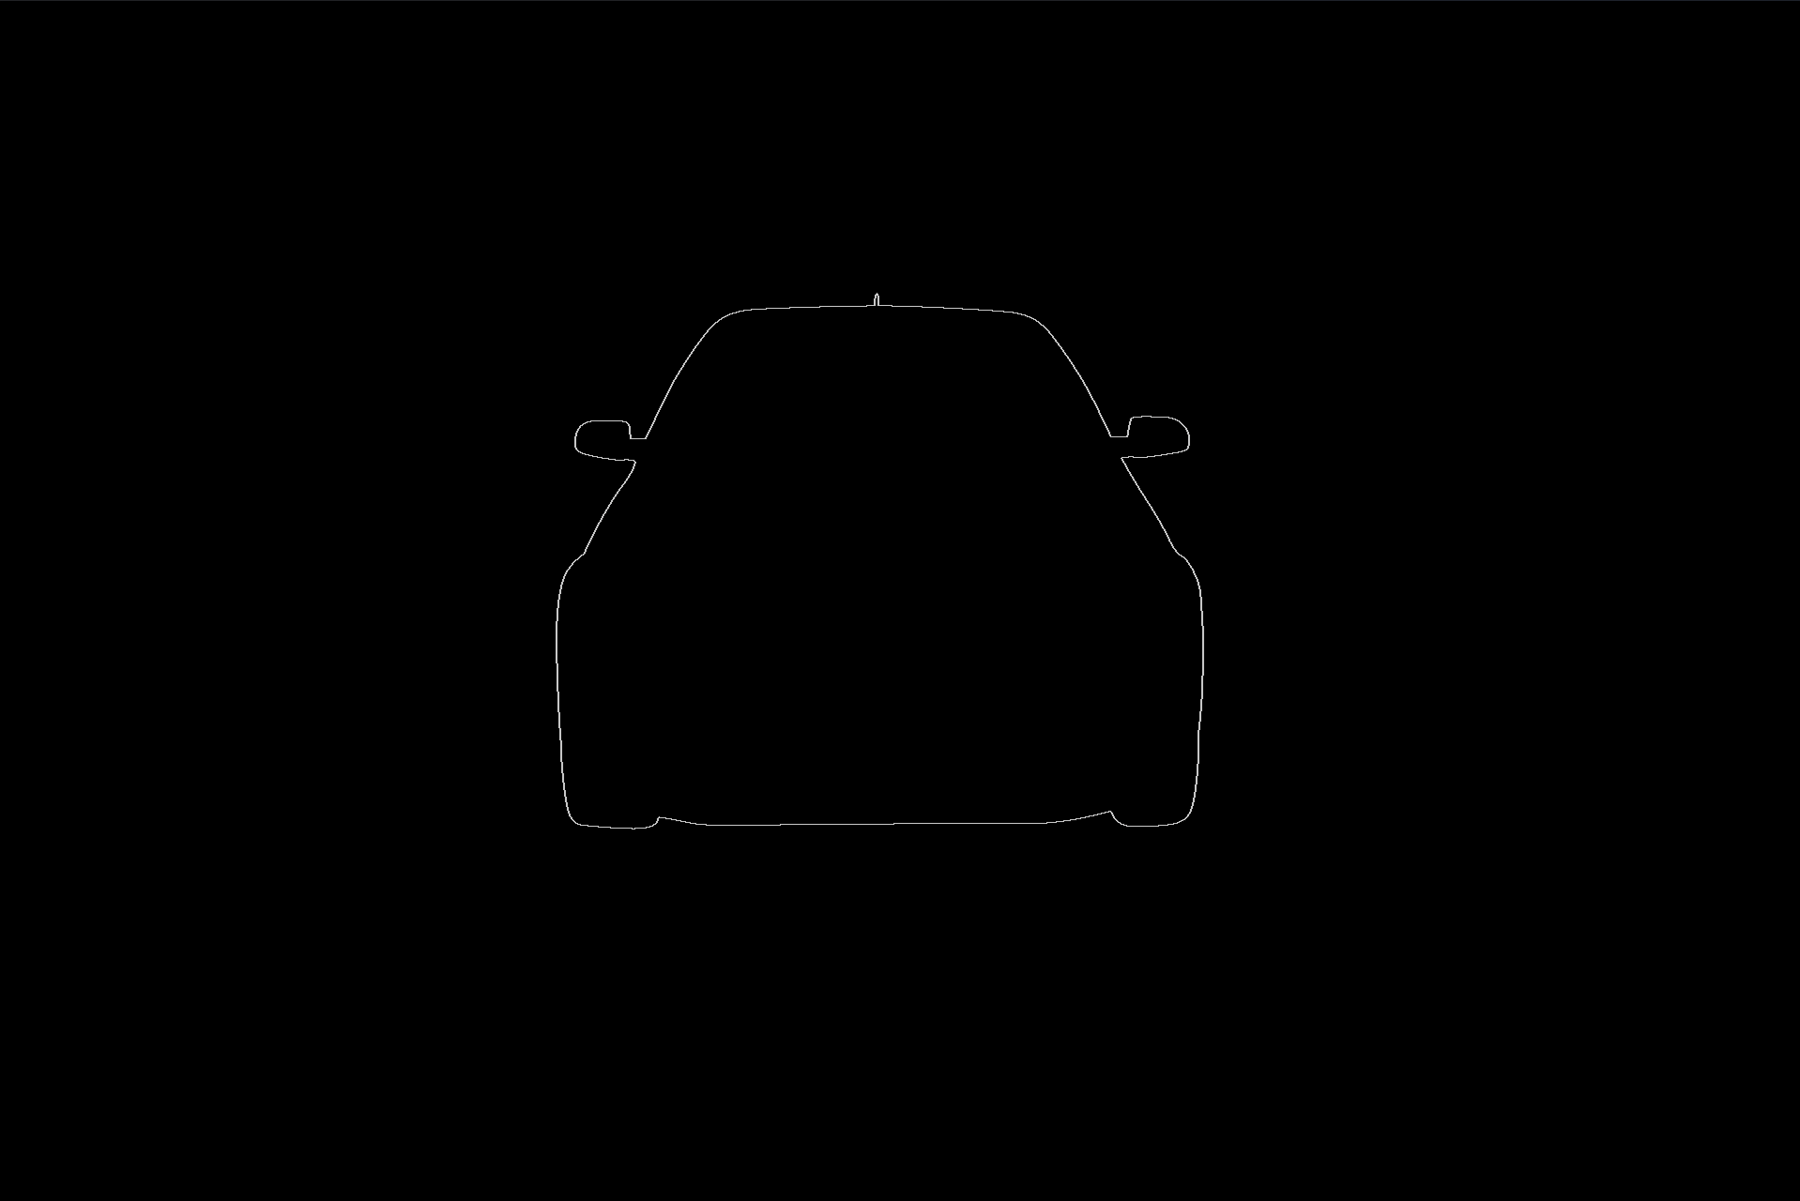
\includegraphics[height=5cm]{edge_outline.png}
        % \caption{edge}
    \end{minipage}
    \caption{mask图和edge图}
    \label{mask_edge_ans}
\end{figure}
模型采用的损失函数如\cref{loss_function}:
\begin{equation}
    loss=CrossEntropy+DiceLoss+EdgeLoss
    \label{loss_function}
\end{equation}

基于通过上面设计的算法提取出的边缘(edge)和轮廓(outline),对边缘和轮廓分别进行加权操作,对比他们的结果。\cref{edge_outline_weight}为具体权重情况对比,\cref{edge_outline_weight_compare}为不同权重的结果对比。\par
\begin{table}[htbp] %表格位置
    \setlength{\abovecaptionskip}{0cm}
    \setlength{\belowcaptionskip}{0.2cm}
    \centering
    \caption{edge和outline不同加权系数比较实验}
    \label{edge_outline_weight}
    \begin{tabular}{|c|c|c|c|c|}
        \hline
        运行名称         & 模型  & EdgeLoss损失项 & edge加权系数 & outline加权系数 \\
        \hline
        dainty-galaxy-30 & U-net & 不添加         & 无           & 无              \\
        \hline
        drawn-pine-44    & U-net & 添加           & 1            & 2               \\
        \hline
        bright-donkey-58 & U-net & 添加           & 1            & 1               \\
        \hline
        sage-music-59    & U-net & 添加           & 1            & 3               \\
        \hline
    \end{tabular}
\end{table}
\begin{figure*}[htbp]
    \centering
    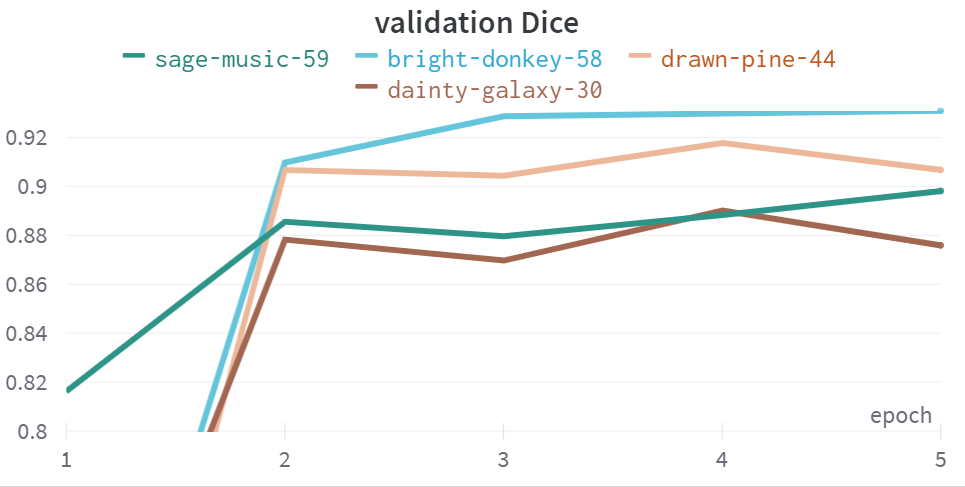
\includegraphics[width=450pt]{edge_outline_weight_compare.png}
    \caption{edge和outline不同加权系数结果比较}
    \label{edge_outline_weight_compare}
\end{figure*}
通过对结果的比较,可以发现不同的加权情况都对结果起到了一定的提升作用。正如前面分析的那样,图像的边缘及围绕边缘的那一圈像素是对实例分割影响比较大的部分,很大程度上影响了对图像的分割效果。
通过对边缘的加权,在模型对边缘分割效果不好时,会导致损失函数增大,对其进行惩罚,从而使得模型更加关注于对边缘的分割效果。在3.5节进行的对比实验中,选择对edge加权为1,outline加权为2来进行实验,并对加了EdgeLoss损失项后对边缘的分割情况进行具体比较。


\section{改进的U-net模型}
对U-net网络模型结构的改进如\cref{model_improve}所示,整体网络模型结构与U-net一样,在此基础上进行了一些改进。

\cref{level1}和\cref{level1_improve}给出了在网络模型在第一层从输入、到第一次下采样池化操作的具体模型比较。
\begin{figure*}[htbp]
    \centering
    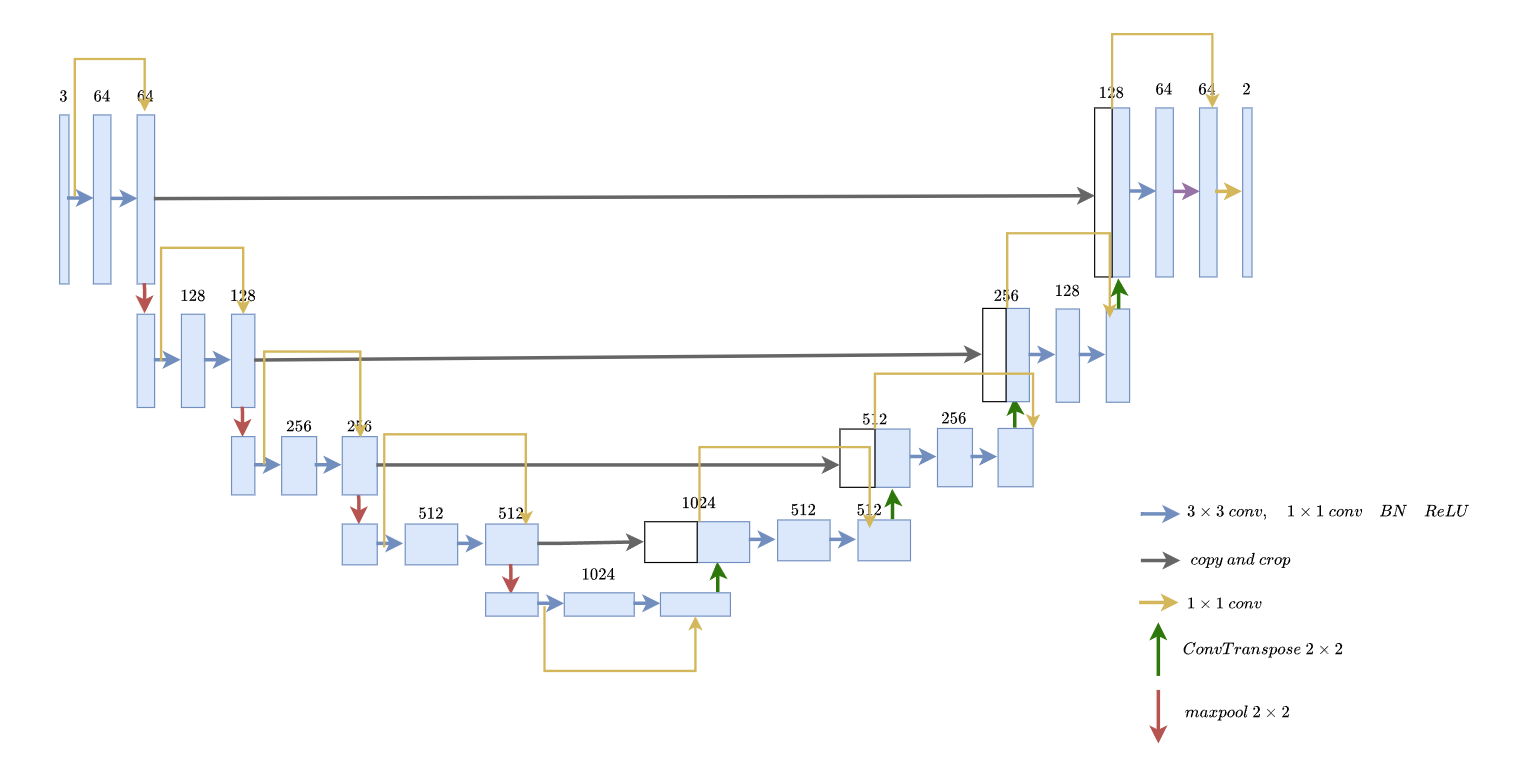
\includegraphics[width=450pt]{u-net_improve2.png}
    \caption{改进的U-net模型结构,矩形上方是对应的通道数}
    \label{model_improve}
\end{figure*}
\begin{figure}[htbp]
    \centering
    \begin{minipage}[t]{0.5\linewidth}  %并排插图时,线宽很重要,自己慢慢试,俩张图就不要超过0.5,三张图不要超过0.33之类的,自己看着办  
        \centering
        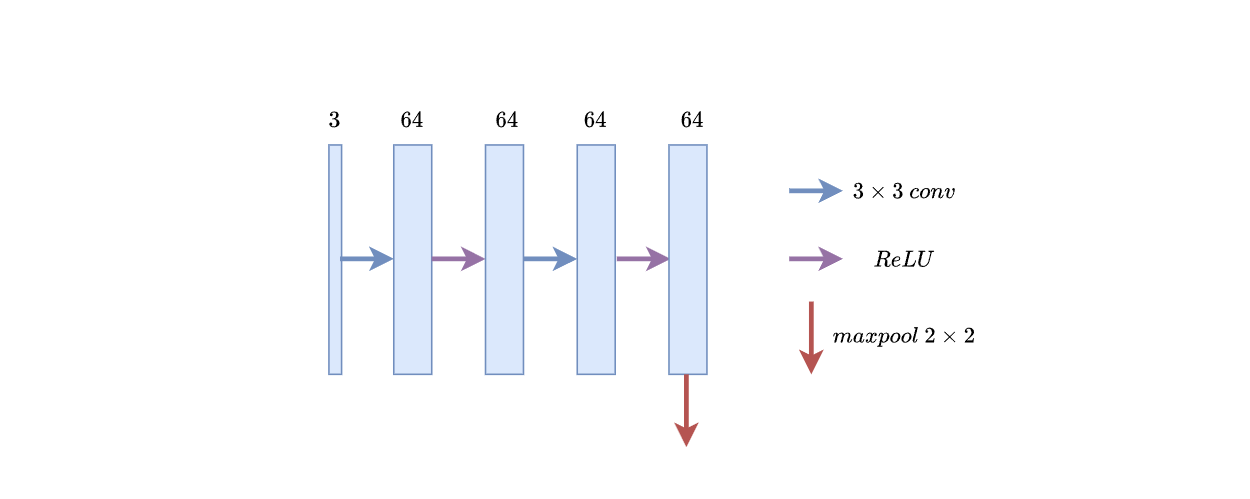
\includegraphics[height=5cm]{level1.png}
        \caption{U-net模型第一层结构}
        \label{level1}
    \end{minipage}
    \hfill%分栏的意思吧
    \begin{minipage}[t]{0.5\linewidth}
        \centering
        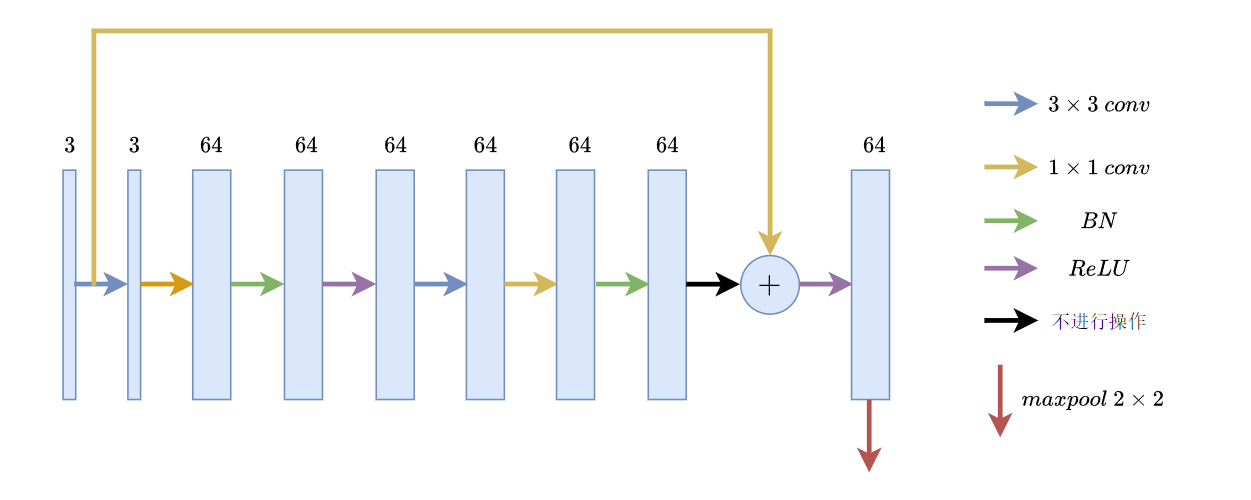
\includegraphics[height=5cm]{level1_improve.png}
        \caption{改进的U-net模型第一层结构}
        \label{level1_improve}
    \end{minipage}
\end{figure}
\par

Sergey Ioffe\textsuperscript{\cite{ioffe2015batch}}等提出了批量规范化层(Batch Normalization,BN),对每一层的输入进行归一化。BN是一种很有效的技术,在训练深度神经网络时,通过对输入进行正则化,可以减轻每一层的变化剧烈程度,加速深层网络的收敛速度。现在的卷积神经网络模型一般都会在卷积操作之后加入批量规范化层。在改进的U-net模型中,在$1\times 1$卷积操作之后,ReLU激活函数前添加BN层,BN层需要学习的拉伸(scale)和偏移(shift)参数。

Resunet\textsuperscript{\cite{zhang2018road}}将残差连接加在批量规范化层之前,同时两次卷积操作与U-net网络相同。对U-net模型的改进参考这一思路将残差连接加在ReLU激活函数之前,同时进一步对网络模型的两次卷积操作进行改进。

在卷积神经网络中,卷积核是主要要通过训练学习得到的参数。卷积核的大小很大程度上影响着卷积神经网络的参数数量。假设输入大小为$w\times h$,卷积核大小为$k_w\times k_h$,在步幅为1的情况下,输出为$(w-k_w+1)\times (h- k_h+1)$,图片的宽度和高度分别减少了$k_w-1$和$k_h-1$,要保证输入大小需要在图片四周分别填充
$[\enspace\lceil \frac{k_w-1}{2}\rceil, \lfloor\frac{k_w-1}{2}\rfloor,\lceil \frac{k_h-1}{2}\rceil, \lfloor\frac{k_h-1}{2}\rfloor\enspace]$ 。在卷积核的大小为奇数时,可以保证在上下和左右填充同样的数量。Szegedy等\textsuperscript{\cite{szegedy2016rethinking}}提出可以用两个连续的$3\times 3$来代替$5\times 5$的卷积核,既可以保证具有相同的感受野范围,同时又减少了所需计算的参数量。\cref{kernel_size_compare}表示了用两个连续$3\times 3$卷积核可以替代$5\times 5$得到相同的提取效果,同时参数量减少了$5\times 5-2\times 3\times 3=7$。

因此,同时出于填充和参数数量的考虑,卷积层一般使用$3\times 3$大小的卷积核。对于更小的$1\times 1$卷积核,其只作用于一个像素,因此不具备提取周围像素特征的能力,但是$1 \times 1$卷积核可以实现不同通道特征的整合,可以对通道数进行调整,同时其所需的参数量非常小。因此,本文打算基于$3\times 3$卷积核和$1\times 1$卷积核来对U-net模型进行改进。
\begin{figure*}[htbp]
    \centering
    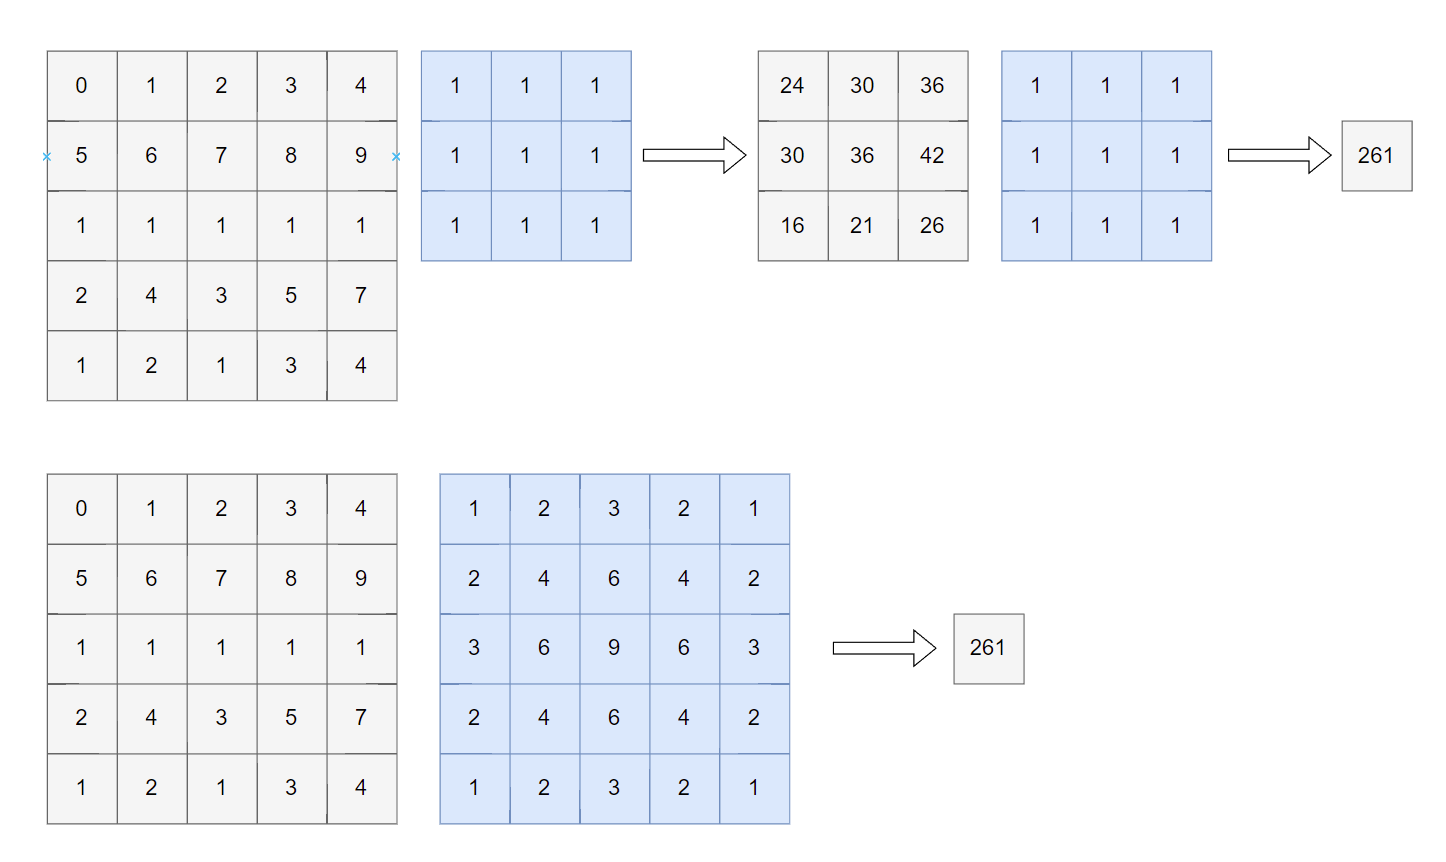
\includegraphics[width=450pt]{kernel_size_compare.png}
    \caption{两个连续$3\times 3$卷积核和$5\times 5$卷积核}
    \label{kernel_size_compare}
\end{figure*}
当网络模型有很多参数时,需要给模型足够数量的样本,在训练的过程中才能不断的拟合这些参数。而小样本要面对样本数量不足的问题,因此要尽量减少模型的参数,同时不影响对图像的分割效果。对于用于卷积层的$3\times 3$卷积核,其形状是一个四维张量$[\mbox{输出通道数, 输入通道数, 卷积核高度}h, \mbox{卷积核宽度}w]$。对应于每一个输出通道,需要输入通道个数的卷积核分别作用于对应的输入通道进行不同通道的融合,并将结果叠加得到一个输出通道的结果。U-net网络模型包括四次下采样,和四次上采样,每一步进行两次$3\times3$卷积核操作。因此$3\times 3$的卷积核所包括的参数个数是当前模型主要需要训练的参数。

输入图像为3通道的RGB图像,U-net的$3\times 3$卷积操作直接将其变为64通道,分析认为每一通道都有其对应的信息,这不利于用卷积操作对每一层特征进行提取。应该先在每一个单独的通道上进行特征提取,然后在结合不同通道的特征,给予其一定的过渡。正如U-net模型对图像的下采样逐步降低输入尺寸,上采样在逐步恢复到图片大小。基于此,对$3\times 3$卷积核进行调整,使得对于每一个输出通道,只用一个卷积核作用于输入通道进行通道特征提取,此时这一操作保证输入通道与输出通道个数相同。对于通道的调整,不同通道特征的融合则通过$1\times 1$的卷积核来实现。下面计算一下他们所需要的参数个数,假设输入通道个数为$C_{in}$,输出通道个数为$C_{out}$:


\begin{equation}
    \begin{split}
        3\times3\mbox{卷积核进行特征提取和通道融合:}C_{out}\times C_{in}\times 3\times 3 \\
        3\times 3\mbox{卷积核特征提取}+ 1\times 1\mbox{通道融合:}C_{in} \times 1 \times 3 \times 3+ C_{out} \times C_{in} \times 1 \times 1\\
        1\times 1\mbox{卷积核进行特征提取和通道融合:}C_{out}\times C_{in}\times 1\times 1
    \end{split}
\end{equation}
\par
以第一层两次卷积操作将输入3通道的RGB图像通过卷积变为64通道为例,计算它们分别的参数个数,其中卷积核都不添加偏置项。同时在两次卷积操作的基础上添加了残差连接,需要将3通道输入用$1\times 1$卷积变为64通道输出,使得其可以与卷积作用的输出进行相加:

\begin{equation}
    \begin{split}
        3\times3\mbox{卷积核进行特征提取和通道融合:}64 \times 3 \times 3 \times 3=1728\\
        64\times 64 \times3\times 3=36864\\
        \mbox{两次}3\times 3\mbox{卷积操作共需参数个数:}1728+36864=38592\\
        3\times 3\mbox{卷积核特征提取}+ 1\times 1\mbox{通道融合:}3 \times 1 \times 3 \times 3+ 64 \times 3 \times 1 \times 1=219 \\
        64\times 1\times 3\times 3+64\times 64\times 1\times1=4672\\
        1\times1\mbox{卷积核进行特征提取和通道融合:}64\times 3\times1 \times 1  =192 \\
        \mbox{两次卷积操作+残差连接共需参数量:}219+4672+192=5083\\
        \frac{38592}{5083}\approx 7.59
        \nonumber
    \end{split}
\end{equation}
\par
通过上面的计算结果,可以发现将$3\times 3$卷积核操作变为$3\times 3卷积核特征提取+ 1\times 1通道融合$可以很大程度上减少网络模型的参数个数。较少的参数个数更有助于在小样本数据集上进行学习,当有较多的参数时,
因为样本数量少,参数的数量大于训练样本特征的维度,很容易导致过拟合的问题。




% \begin{figure}[htbp]
%     \begin{minipage}[t]{0.5\linewidth}  %并排插图时,线宽很重要,自己慢慢试,俩张图就不要超过0.5,三张图不要超过0.33之类的,自己看着办  
%         \centering
%         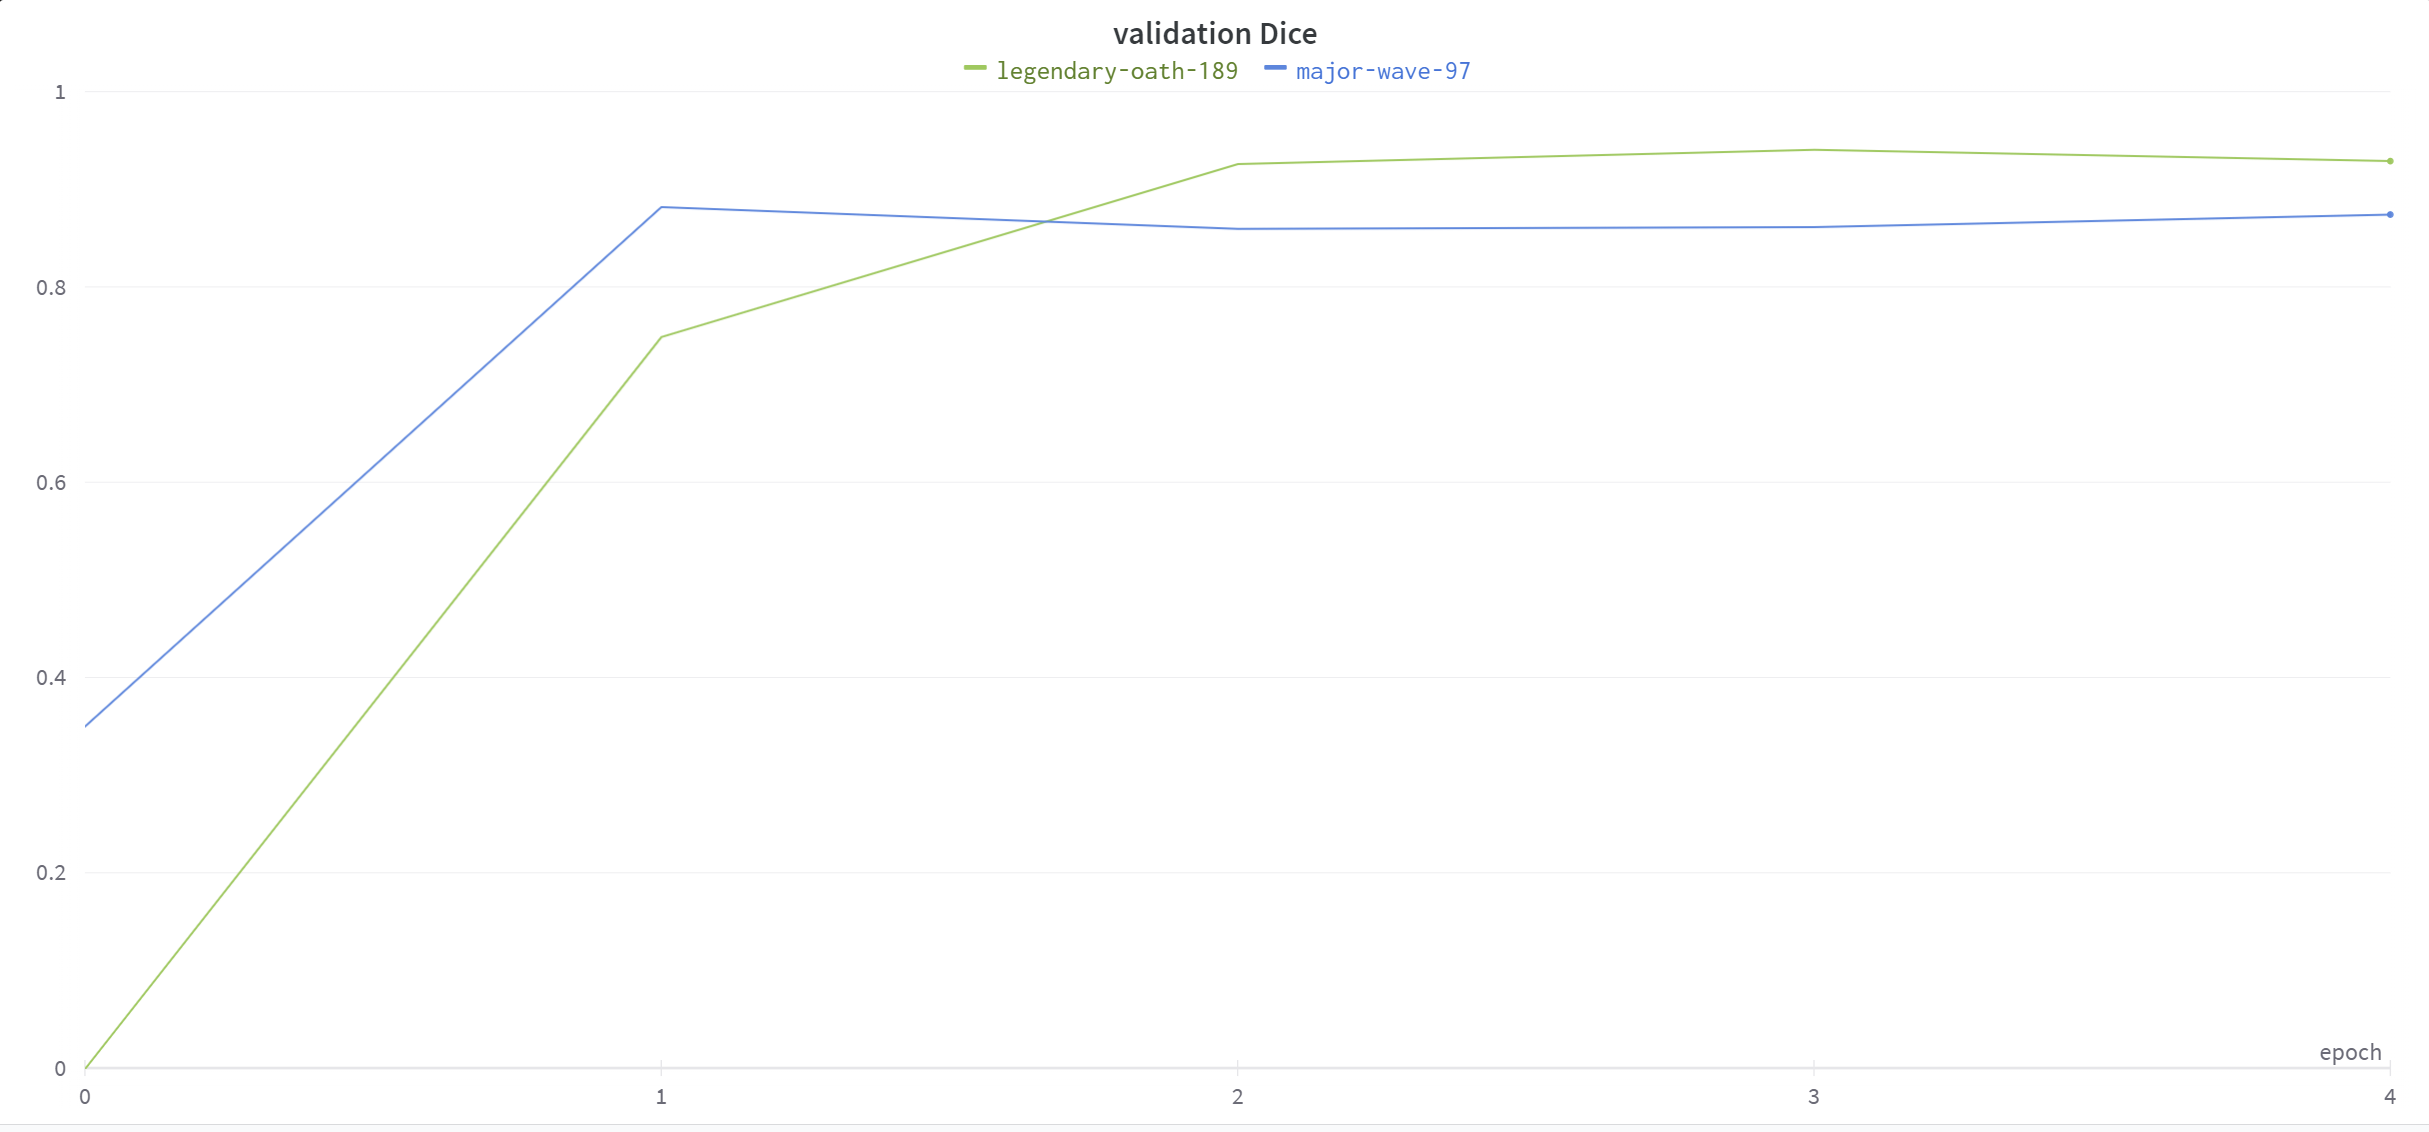
\includegraphics[height=4cm]{model_compare.png}
%         \label{model_compare}
%         \caption{验证集Dice相似系数}
%     \end{minipage}
%     \hfill%分栏的意思吧
%     \begin{minipage}[t]{0.5\linewidth}
%         \centering
%         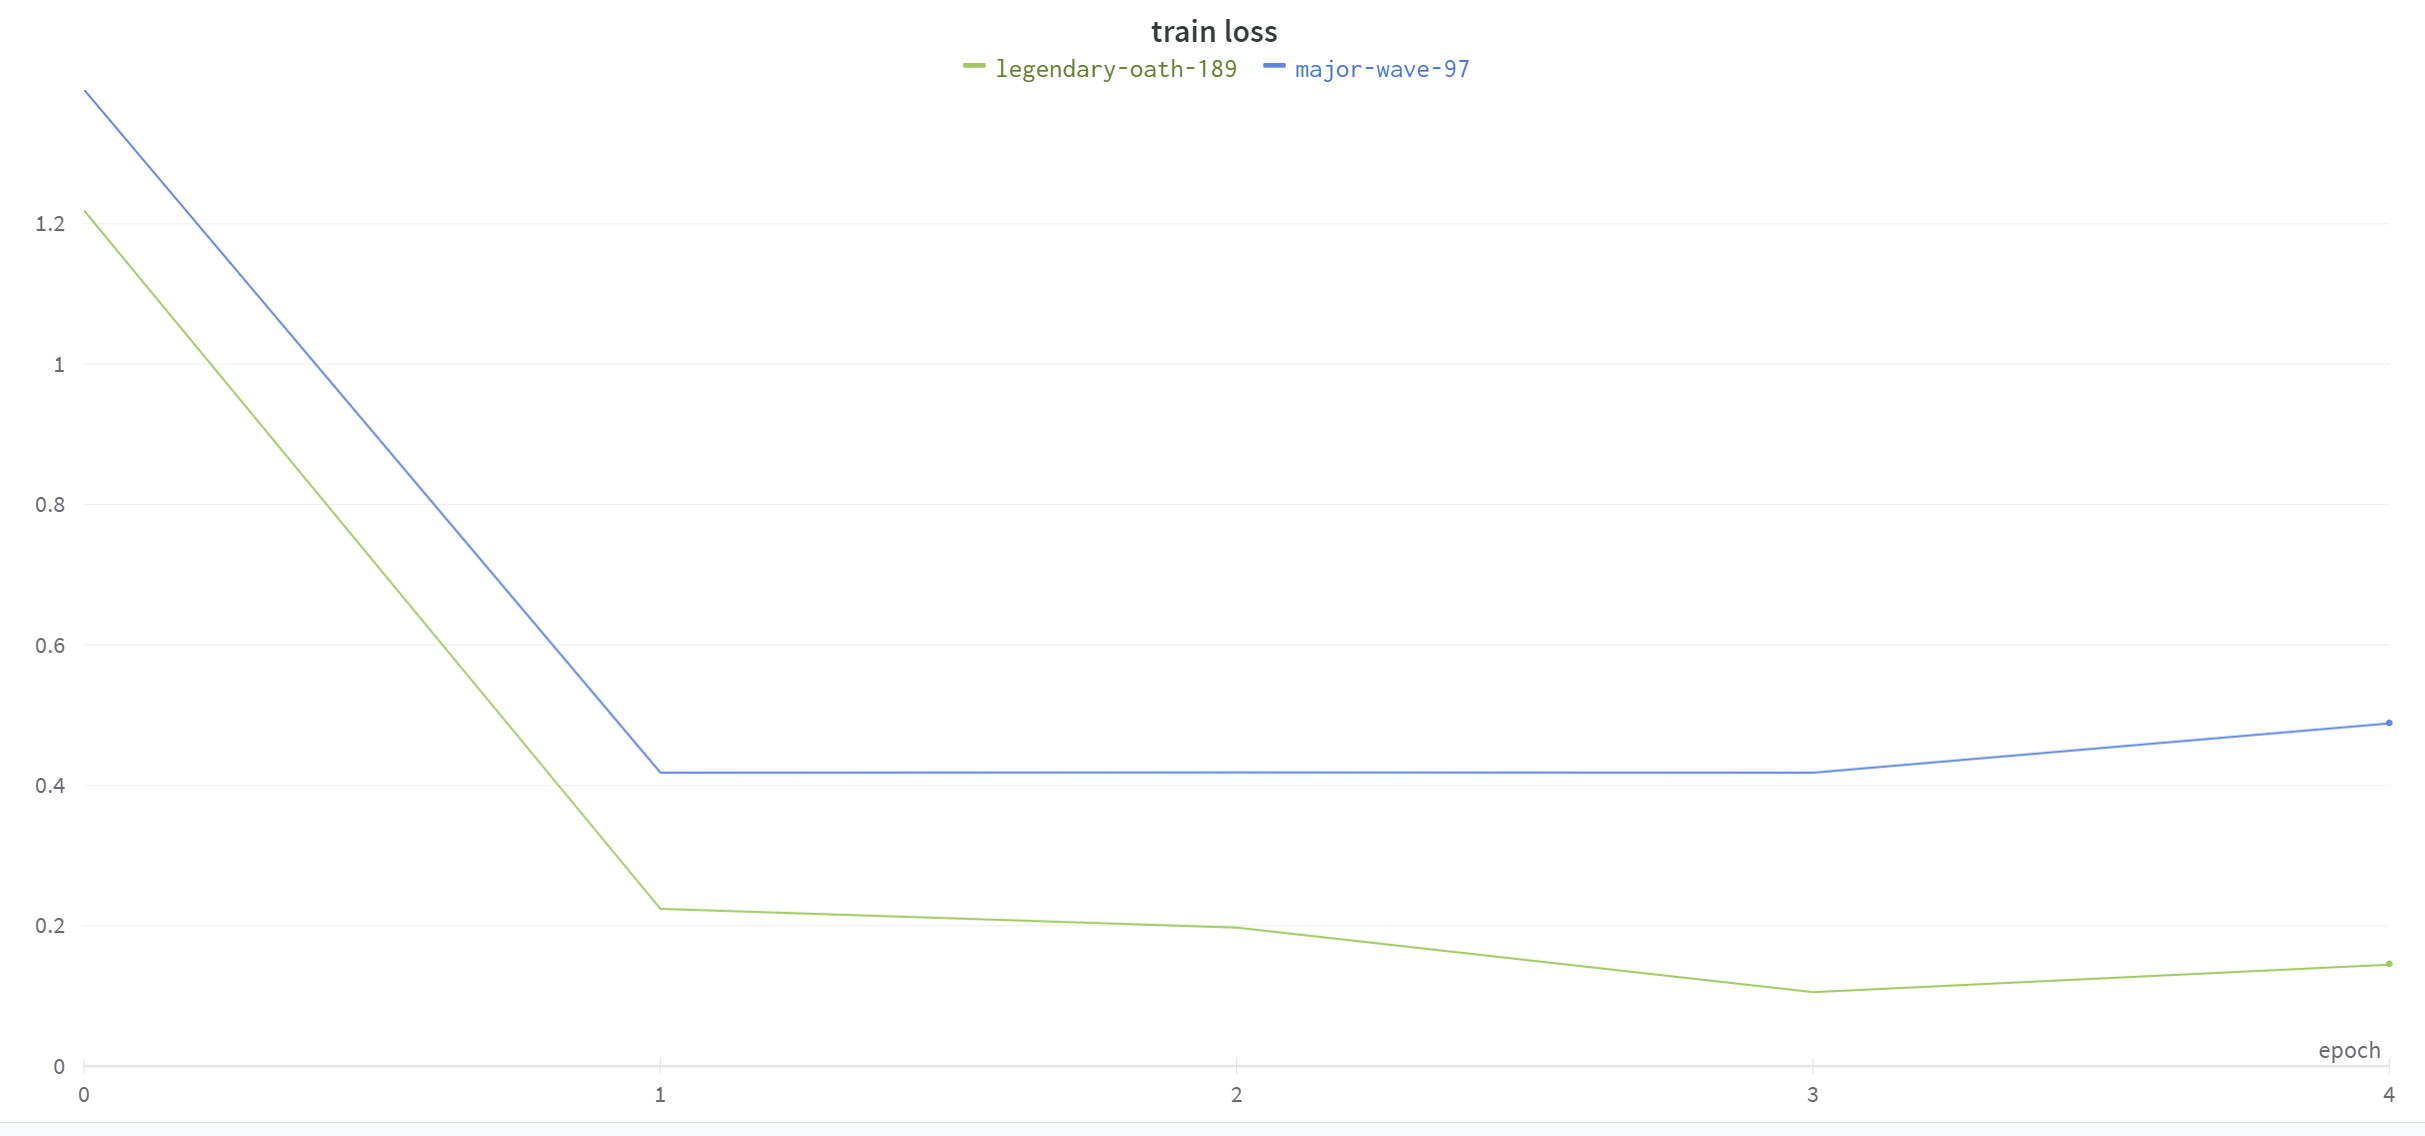
\includegraphics[height=4cm]{model_loss.png}
%         \label{model_loss}
%         \caption{训练损失}
%     \end{minipage}
% \end{figure}


\section{实验结果和分析}
基于上面提出的小样本图像分割的解决方案,进行数据增强、添加EdgeLoss损失项提高模型对边缘的敏感度、改进U-net模型,设计对比实验验证它们的效果,
在这里进行数据增强操作是通过3.1节分析确定的5种数据增强操作(hflip、rotate、affineScale、ColorJitter\_hue0.5、ColorJitter\_contrast0.5)。
在前面已经分析验证了数据增强操作的有效性,这里不对数据增强操作在单独进行对照实验。
\cref{compare_experiment}分别给出了对应的训练运行名称和进行的相应操作。
\begin{table}[htbp] %表格位置
    \setlength{\abovecaptionskip}{0cm}
    \setlength{\belowcaptionskip}{0.2cm}
    \centering
    \caption{分析对比实验设计}
    \label{compare_experiment}
    \begin{tabular}{|c|c|c|c|}
        \hline
        运行名称            & 数据增强 & EdgeLoss损失项 & 模型      \\
        \hline
        dainty-galaxy-30    & 否       & 不添加         & U-net     \\
        \hline
        drawn-pine-44       & 否       & 添加           & U-net     \\
        \hline
        floral-paper-48     & 是       & 不添加         & U-net     \\
        \hline
        crimson-morning-49  & 是       & 添加           & U-net     \\
        \hline
        preety-butterfly-53 & 否       & 不添加         & 改进U-net \\
        \hline
        ethereal-hill-54    & 是       & 不添加         & 改进U-net \\
        \hline
        dulcet-sun-56       & 否       & 添加           & 改进U-net \\
        \hline
        fresh-glade-55      & 是       & 添加           & 改进U-net \\
        \hline
    \end{tabular}
\end{table}



\subsection{EdgeLoss损失项对照实验}


为了验证在损失函数中添加EdgeLoss项后对图像分割效果的影响,进行对照实验验证其结果。同时为了保证在进行数据增强与不进行数据增强情况下,添加EdgeLoss损失项对结果是否都有提升。分别进行数据增强与不进行数据增强操作,这里的实验变量为是否进行数据增强操作,以及是否添加EdgeLoss损失项,同时对于学习率、训练迭代次数等超参数的设置保持一致。
采用Dice相似系数作为模型的评估指标,\cref{edgeloss_compare_no_aug}和\cref{edgeloss_compare_aug}所示分别为不进行数据增强操作和进行数据增强操作时,在损失函数中是否添加EdgeLoss项的对比情况。

其中drawn-pine-44、dainty-galaxy-30为不进行数据增强操作,crimson-morning-49、floral-paper-48进行上节提到的5种数据增强操作。
dainty-galaxy-30和floral-paper-48都未添加EdgeLoss损失函数项。
通过对实验结果的比较可以发现,在进行数据增强操作与不进行数据增强操作的情况下,当在损失函数中添加EdgeLoss这一项后,在验证集上的Dice相似系数都比不添加EdgeLoss要高。这说明了添加了这一损失函数项,使模型的性能得以提升。
\begin{figure}[htbp]
    \centering
    \begin{minipage}[t]{0.45\linewidth}  %并排插图时,线宽很重要,自己慢慢试,俩张图就不要超过0.5,三张图不要超过0.33之类的,自己看着办  
        \centering
        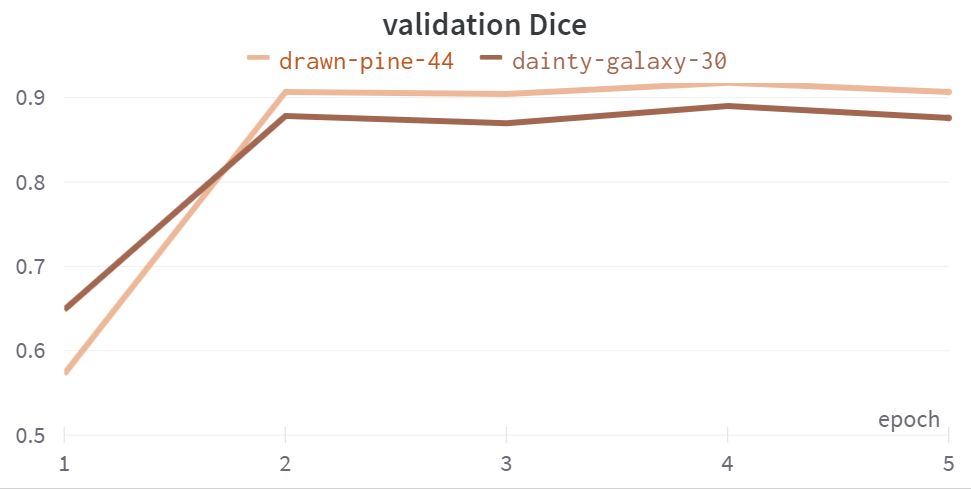
\includegraphics[height=4cm]{edgeloss_compare_no_aug.png}
        \caption{不进行数据增强操作,EdgeLoss对照结果}
        \label{edgeloss_compare_no_aug}
    \end{minipage}
    \hfill%分栏的意思吧
    \begin{minipage}[t]{0.45\linewidth}
        \centering
        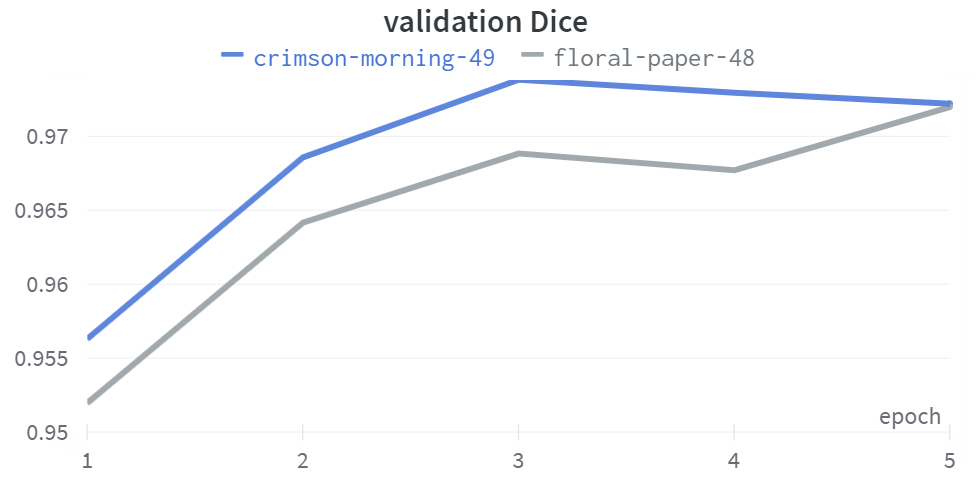
\includegraphics[height=4cm]{edgeloss_compare_aug.png}
        \caption{进行数据增强操作,EdgeLoss对照结果}
        \label{edgeloss_compare_aug}
    \end{minipage}
    % \caption{mask图和edge图}
\end{figure}
% \begin{figure*}
%     \centering
%     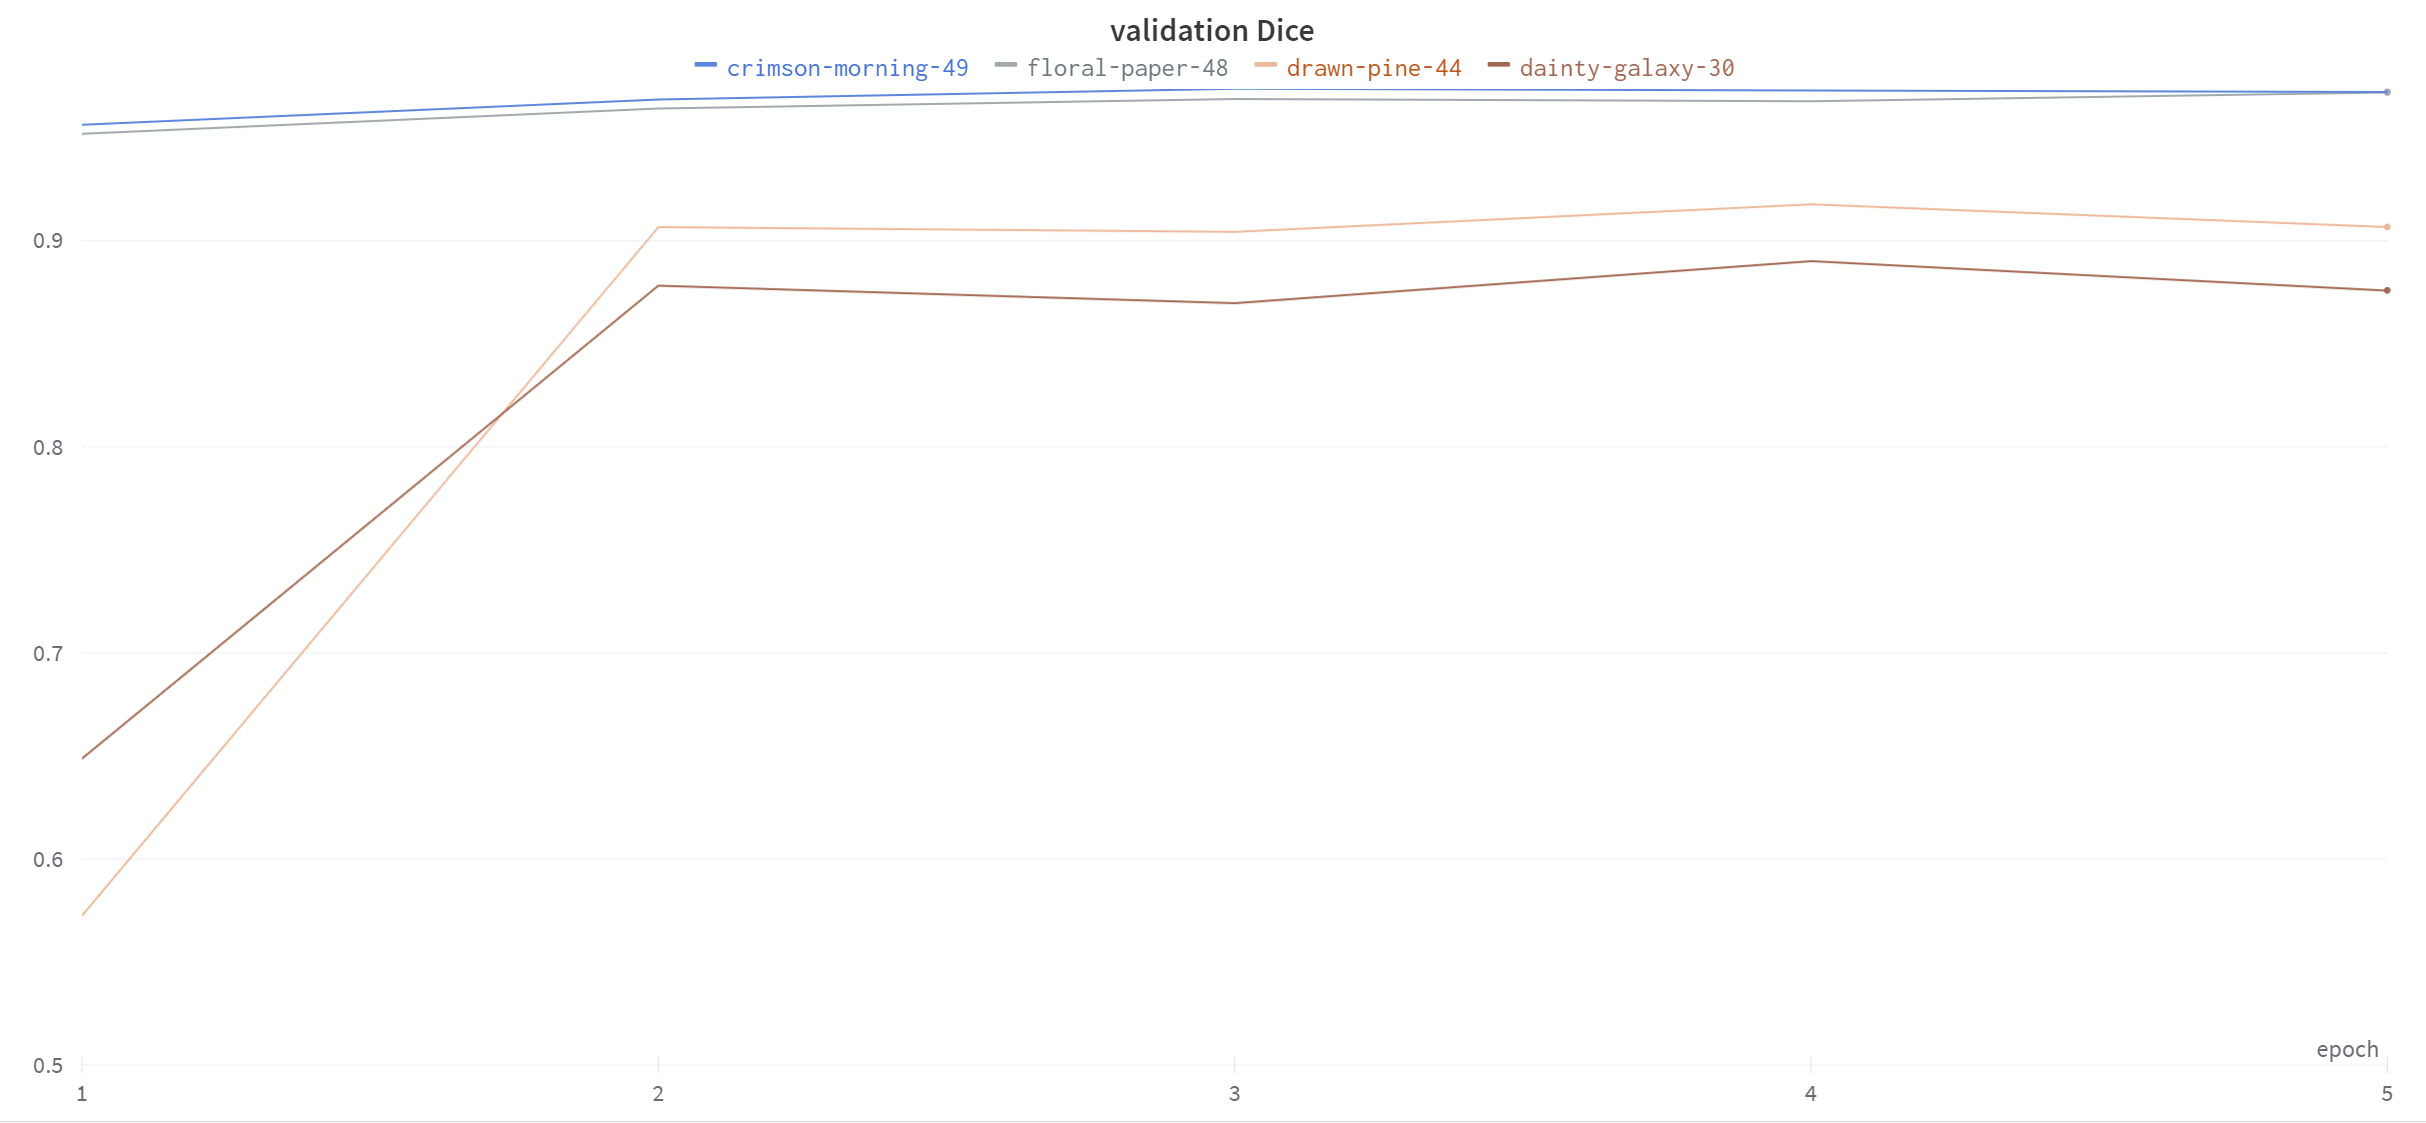
\includegraphics[width=350pt]{edgeloss_compare.png}
%     \caption{在损失函数中添加EdgeLoss损失项与不添加这一项时的结果}
%     \label{edgeloss_compare}
% \end{figure*}


% \begin{figure}[htbp]
%     \centering
%     \begin{minipage}[t]{0.22\linewidth}  %并排插图时,线宽很重要,自己慢慢试,俩张图就不要超过0.5,三张图不要超过0.33之类的,自己看着办  
%         % \centering
%         \includegraphics[height=3cm]{mask_image.jpg}
%         \caption{原始图像}
%     \end{minipage}
%     \hfill%分栏的意思吧
%     \begin{minipage}[t]{0.22\linewidth}
%         % \centering
%         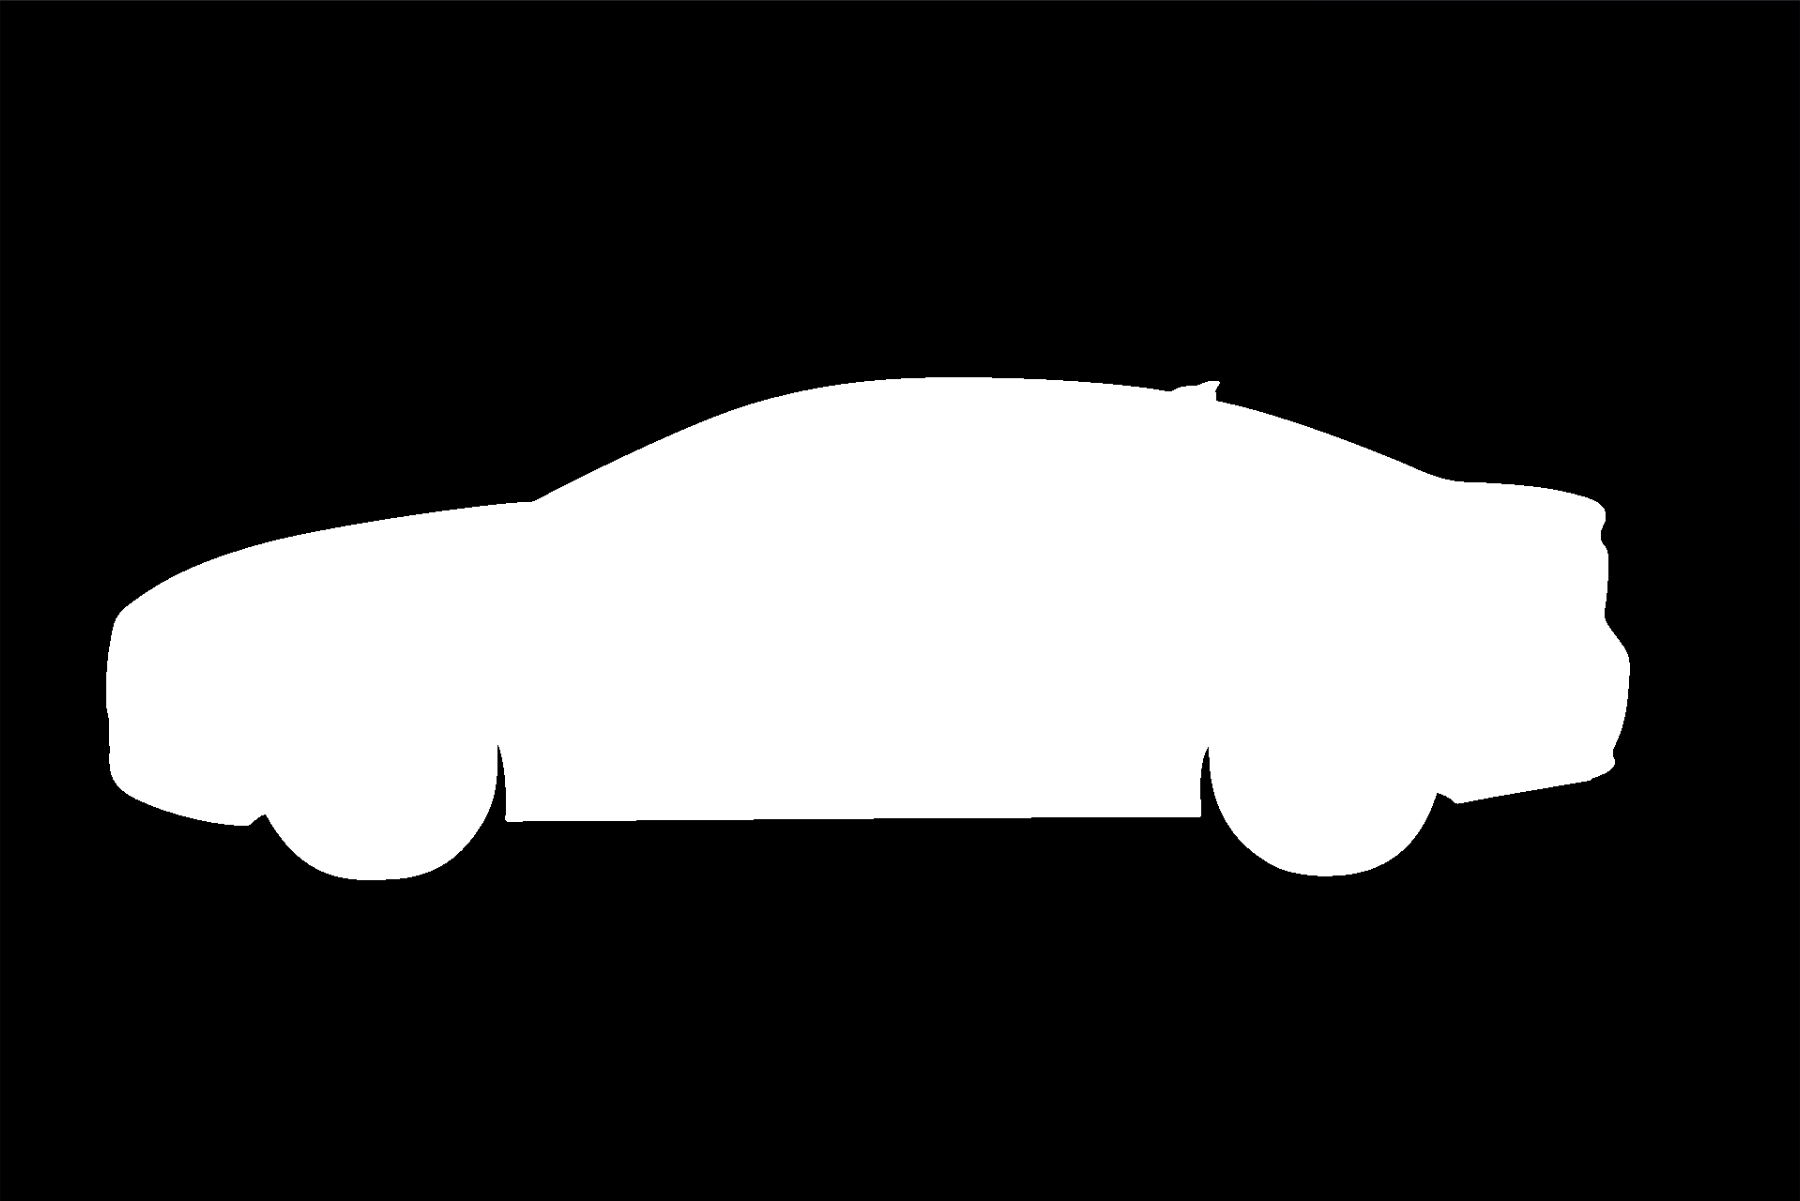
\includegraphics[height=3cm]{mask_true.png}
%         \caption{真实分割图}
%     \end{minipage}

%     \hfill%分栏的意思吧
%     \begin{minipage}[t]{0.22\linewidth}
%         % \centering
%         \includegraphics[height=3cm]{mask_edge.jpg}
%         \caption{添加EdgeLoss项}
%     \end{minipage}

%     \hfill%分栏的意思吧
%     \begin{minipage}[t]{0.22\linewidth}
%         % \centering
%         \includegraphics[height=3cm]{mask_noedge.jpg}
%         \caption{不添加EdgeLoss项}
%     \end{minipage}

%     \caption{分割图对比}
%     \label{mask_compare}
% \end{figure}


% \begin{figure}[htbp]
%     \centering
%     \subfloat[原始图像]{
%         \begin{minipage}[t]{0.5\linewidth}
%             \centering
%             \includegraphics[width=6cm]{mask_image.jpg}
%             %\caption{fig1}
%         \end{minipage}%
%     }%
%     \subfloat[真实分割图]{
%         \begin{minipage}[t]{0.5\linewidth}
%             \centering
%             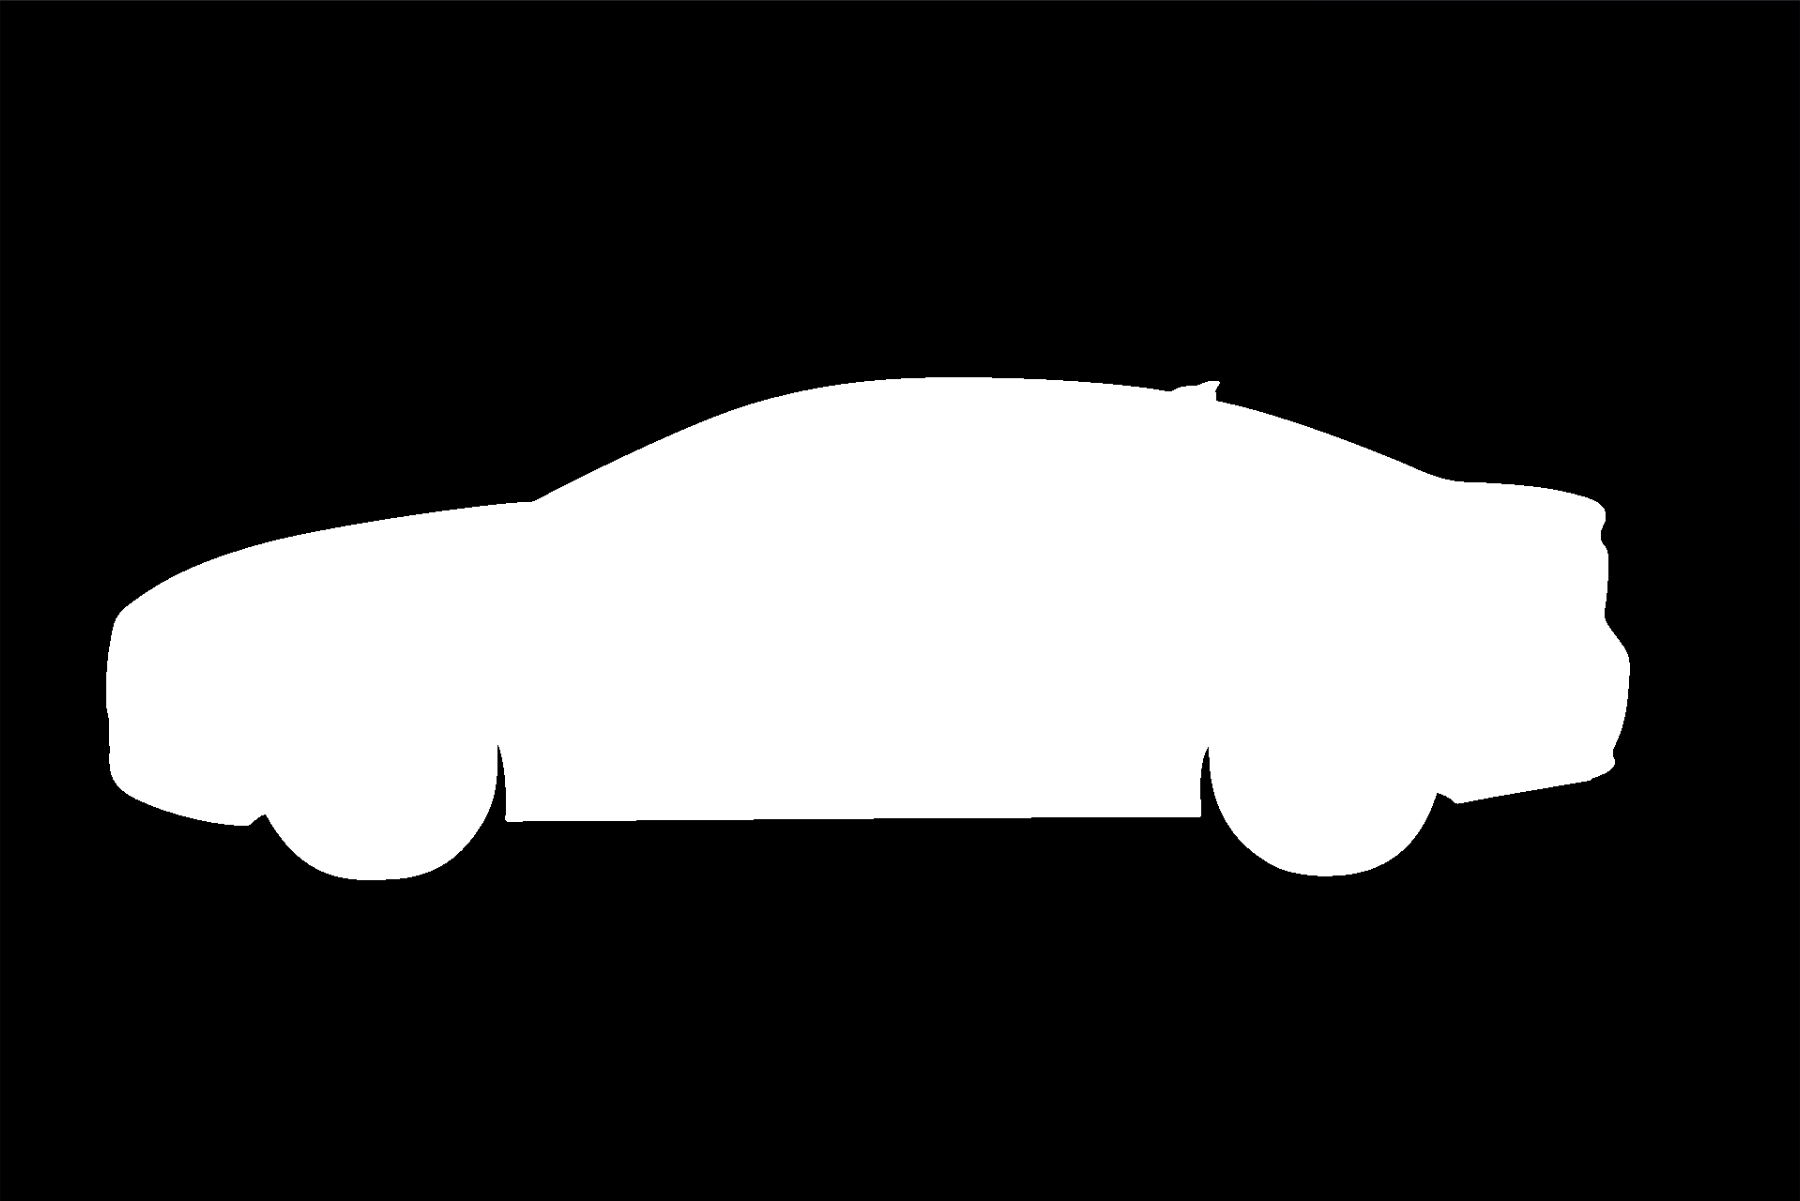
\includegraphics[width=6cm]{mask_true.png}
%             %\caption{fig2}
%         \end{minipage}%
%     }%
%     \quad
%     \subfloat[添加EdgeLoss项]{
%         \begin{minipage}[t]{0.5\linewidth}
%             \centering
%             \includegraphics[width=6cm]{mask_edge.jpg}
%             %\caption{fig2}
%         \end{minipage}
%     }%
%     \subfloat[不添加EdgeLoss项]{
%         \begin{minipage}[t]{0.5\linewidth}
%             \centering
%             \includegraphics[width=6cm]{mask_noedge.jpg}
%             %\caption{fig2}
%         \end{minipage}
%     }%
%     \centering
%     \caption{分割图对比}
%     \label{mask_compare}
% \end{figure}
\begin{figure}[htbp]
    \centering
    \subfloat[原始图像]{
        \begin{minipage}[t]{1.0\linewidth}
            \centering
            \includegraphics[width=5cm]{mask_image.jpg}
            \includegraphics[width=5cm]{mask_image1.jpg}
            \includegraphics[width=5cm]{mask_image2.jpg}
            %\caption{fig1}
        \end{minipage}%
    }%
    \quad
    \subfloat[真实分割图]{
        \begin{minipage}[t]{1.0\linewidth}
            \centering
            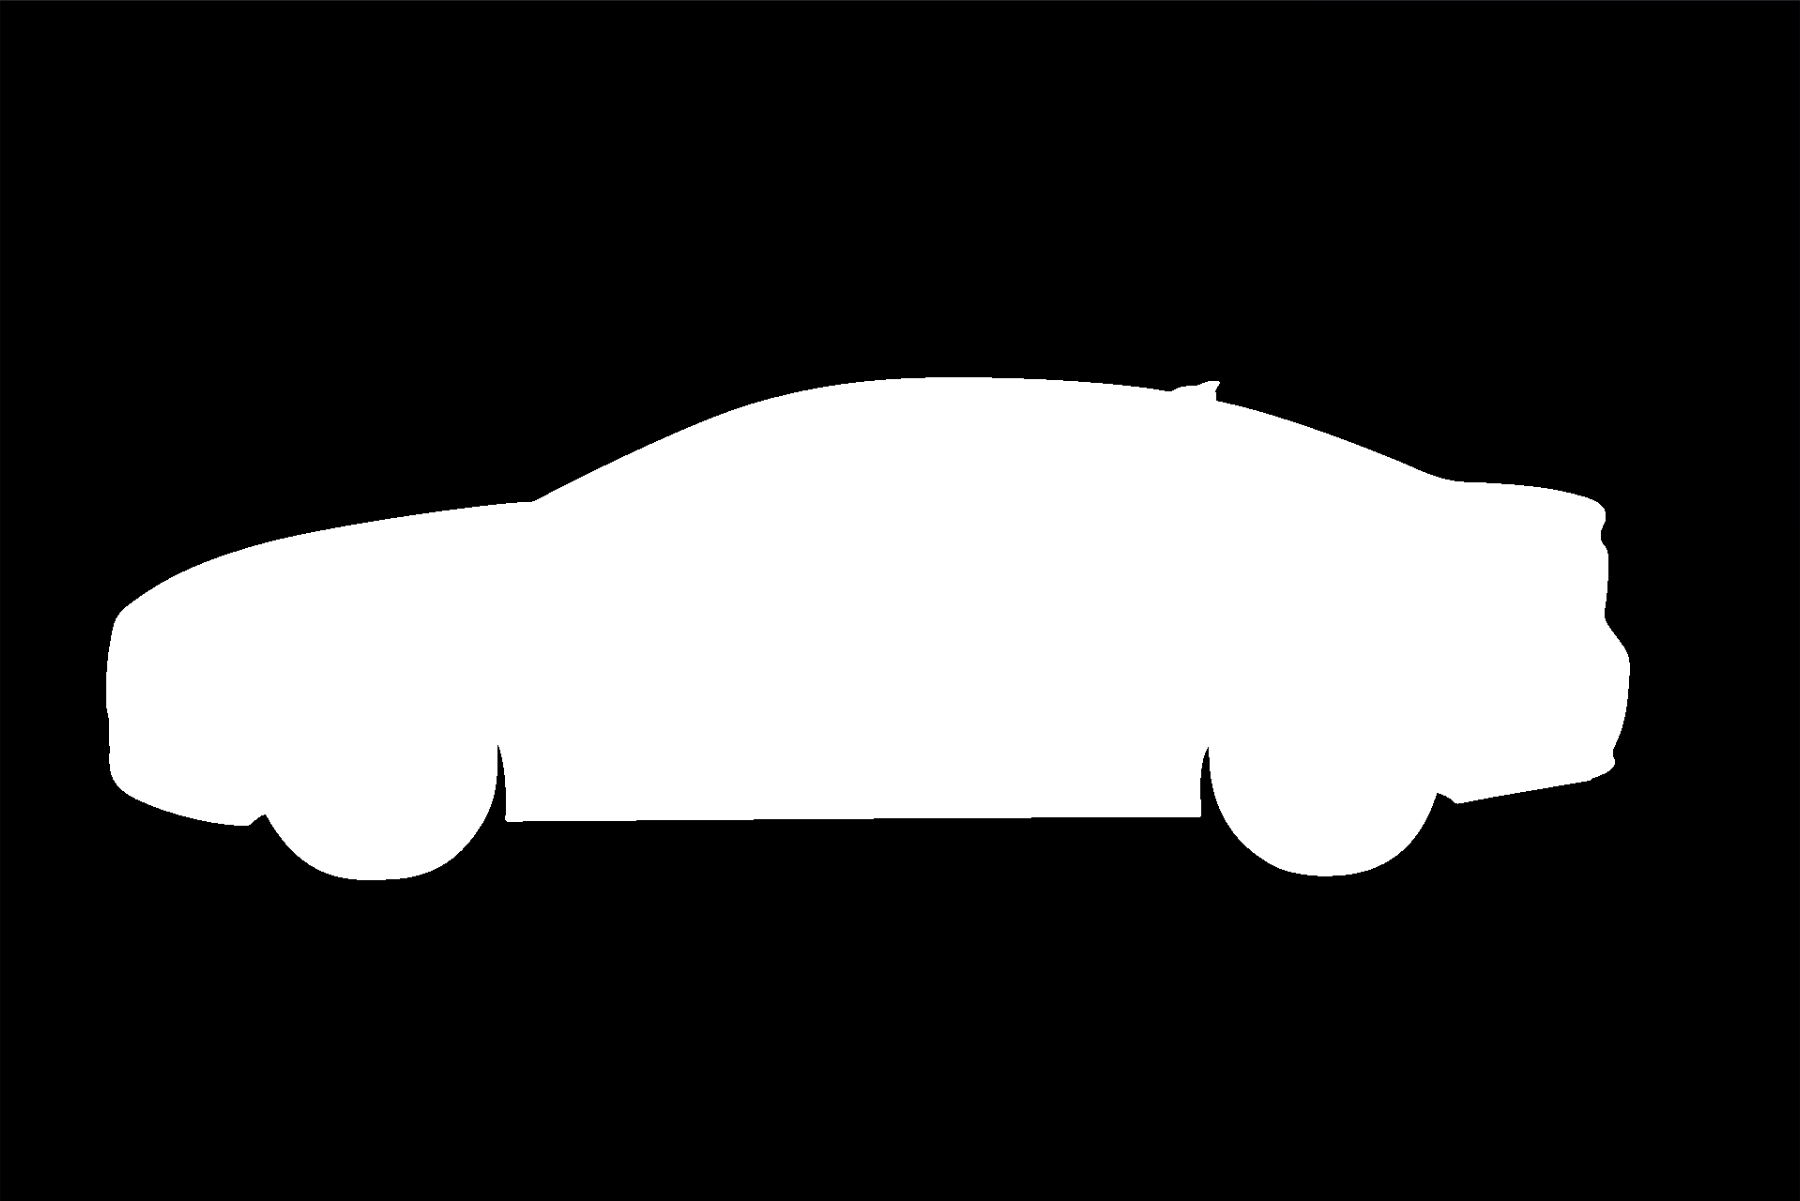
\includegraphics[width=5cm]{mask_true.png}
            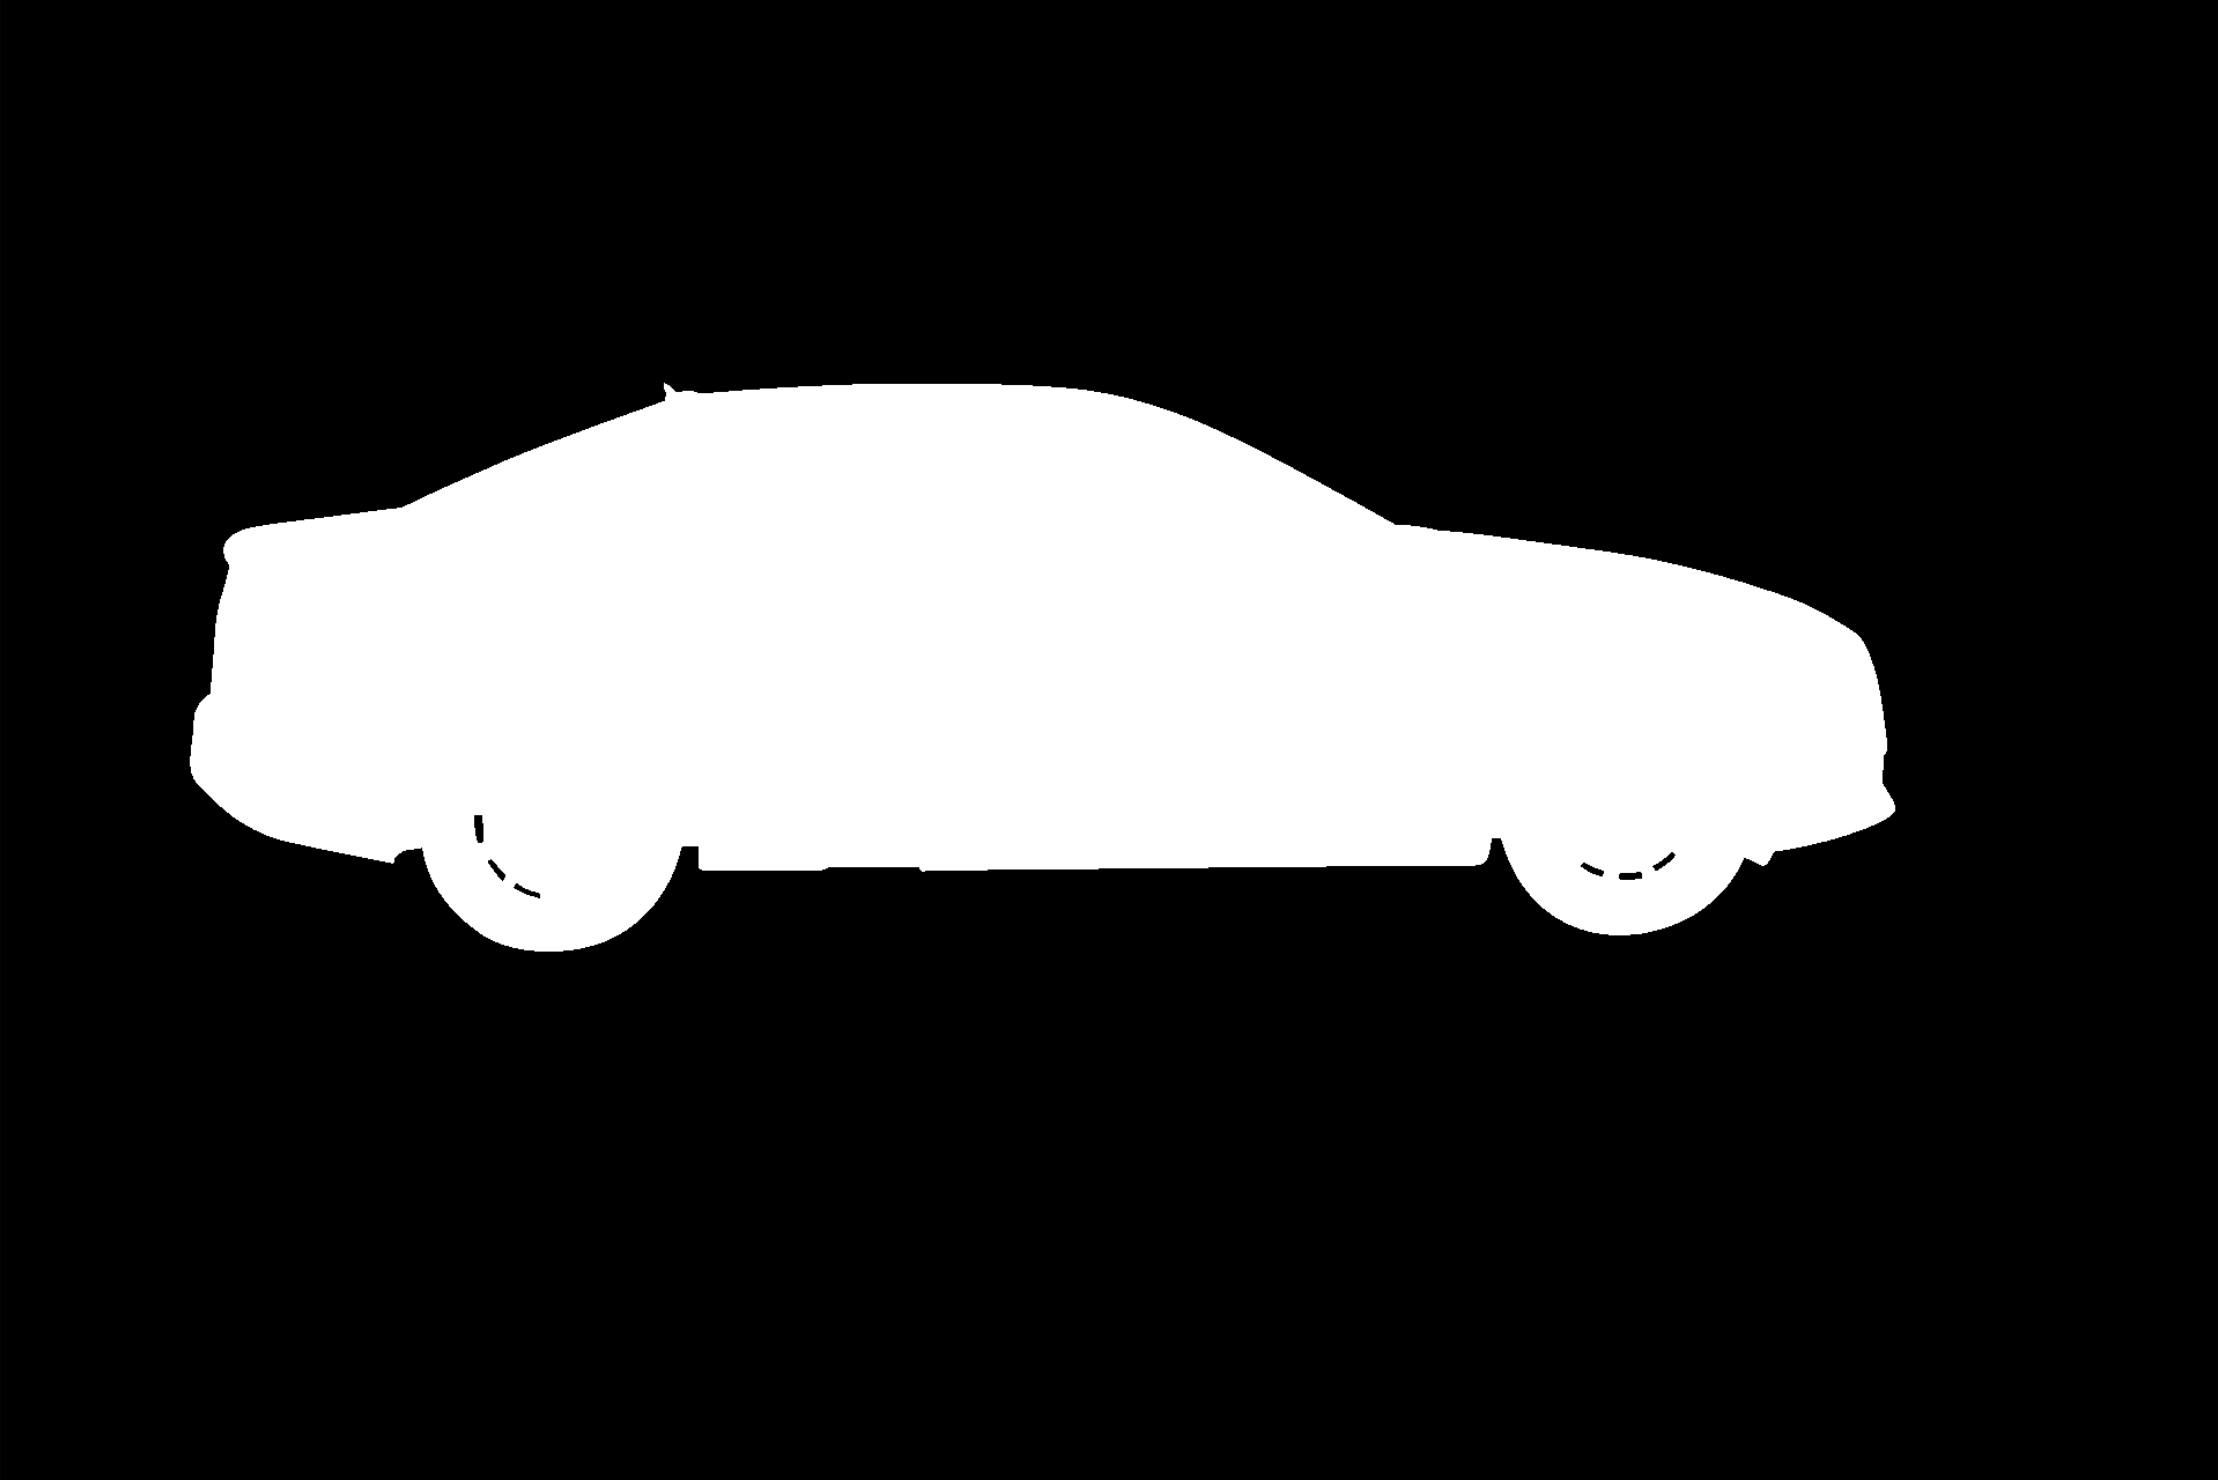
\includegraphics[width=5cm]{mask_true1.png}
            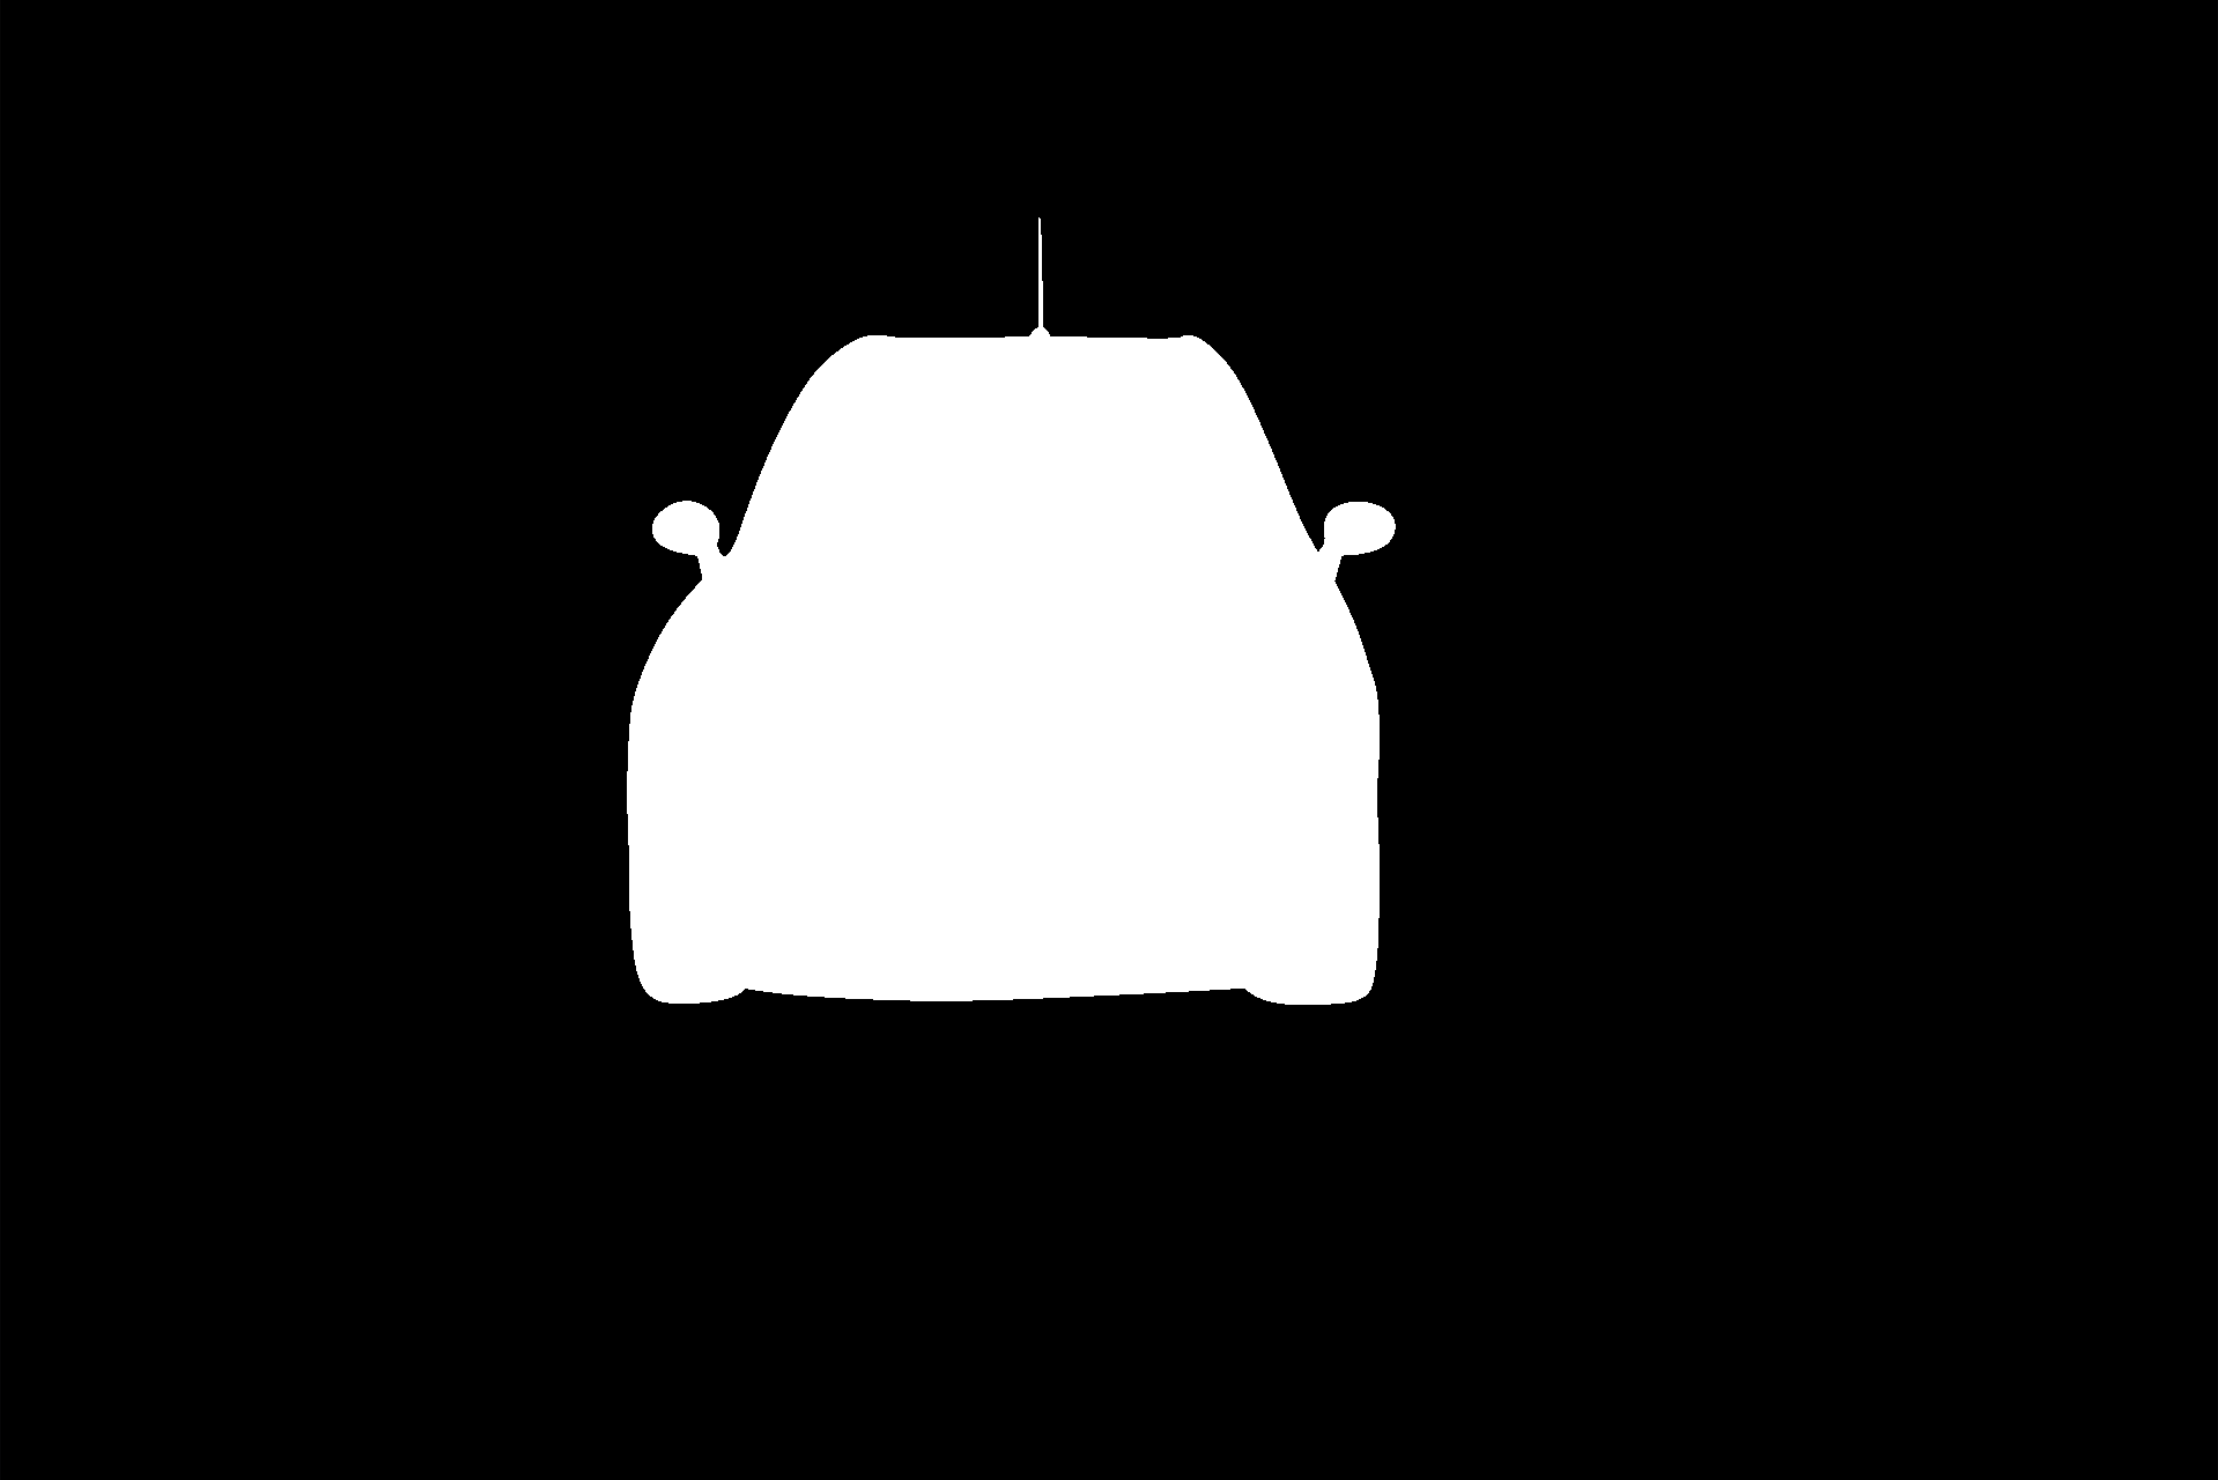
\includegraphics[width=5cm]{mask_true2.png}
            %\caption{fig2}
        \end{minipage}%
    }%
    \quad
    \subfloat[添加EdgeLoss项]{
        \begin{minipage}[t]{1.0\linewidth}
            \centering
            \includegraphics[width=5cm]{mask_edge.jpg}
            \includegraphics[width=5cm]{mask_edge1.jpg}
            \includegraphics[width=5cm]{mask_edge2.jpg}
            %\caption{fig2}
        \end{minipage}
    }%
    \quad
    \subfloat[不添加EdgeLoss项]{
        \begin{minipage}[t]{1.0\linewidth}
            \centering
            \includegraphics[width=5cm]{mask_noedge.jpg}
            \includegraphics[width=5cm]{mask_noedge1.jpg}
            \includegraphics[width=5cm]{mask_noedge2.jpg}
            %\caption{fig2}
        \end{minipage}
    }%
    \centering
    \caption{用U-net模型进行训练,模型分割图对比}
    \label{mask_compare}
\end{figure}

更近一步,可以比较添加这一项与不添加这一项时对图像的边缘分割情况,\cref{mask_compare}显示了他们之间的对比情况,其中红框标识出了添加EdgeLoss损失项后对边缘细节的处理,
可以发现添加了EdgeLoss损失项后对边缘的分割效果更好,同时对图像的分割出了一些在不添加EdgeLoss损失项时所没有的细节。
通过在损失函数中添加了EdgeLoss项,使得模型对边缘的分割效果更加敏感。当模型对边缘的分割效果不好时,EdgeLoss项使得损失函数增大,从而使得模型更多的关注于边缘的分割。但同时也发现,添加了这一项后使得模型对细节较为敏感,从而在实例的周围形成了一些错误的分割情况。但总体上,通过Dice相似系数进行评估,模型的性能得到了一定的提升。






\subsection{改进U-net模型对照实验}
为了验证改进的U-net模型是否有助于提高在验证集上的图像分割效果,在进行数据增强与不进行数据增强时分别比较U-net模型与改进U-net模型在验证集上的Dice相似系数,
以证明在数据增强与不进行数据增强的情况下,改进U-net模型都有助于提升图像分割精确度,改善模型效果。

\cref{model_dice_no_aug}和\cref{model_dice_aug}所示分别为不进行数据增强操作和进行数据增强操作时,改进的U-net模型和U-net在验证集上的表现情况。
floral-paper-48和ethereal-hill-54进行数据增强操作。ethereal-hill-54和pretty-butterfly-53是在改进U-net模型上训练的结果,
floral-paper-48和dainty-galaxy-30是在U-net模型上训练的结果。通过对结果的比较,改进的U-net模型在测试集得到了较高的Dice相似系数,取得了比较好的效果。
改进的U-net模型通过引入了残差连接,同时减少了模型的参数量。残差连接使得输入可以更快的向前传播,同时较少的参数个数更有助于在小样本数据集上进行学习,当有较多的参数时,
因为样本数量少,参数的数量大于训练样本特征的维度,很容易导致过拟合的问题。


\begin{figure}[htbp]
    \centering
    \begin{minipage}[t]{0.45\linewidth}  %并排插图时,线宽很重要,自己慢慢试,俩张图就不要超过0.5,三张图不要超过0.33之类的,自己看着办  
        \centering
        \includegraphics[height=4cm]{model_dice_no_aug.png}
        \caption{不进行数据增强操作,改进U-net对照结果}
        \label{model_dice_no_aug}
    \end{minipage}
    \hfill%分栏的意思吧
    \begin{minipage}[t]{0.45\linewidth}
        \centering
        \includegraphics[height=4cm]{model_dice_aug.png}
        \caption{进行数据增强操作,改进U-net对照结果}
        \label{model_dice_aug}
    \end{minipage}
    % \caption{mask图和edge图}
\end{figure}
% \begin{figure*}
%     \centering
%     \includegraphics[width=400pt]{model_dice.png}
%     \caption{U-net和改进U-net的表现效果}
%     \label{model_dice}
% \end{figure*}

\subsection{同时添加EdgeLoss与改进U-net对照实验}
最后,同时在损失函数中添加EdgeLoss损失项,并采用改进的U-net模型来进行实验,已验证将两者结合时不会对模型的性能产生负面影响。并分别在进行数据增强与不进行数据增强时进行对比实验。\cref{u-net_improve_edgeloss_compare}和\cref{u-net_improve_aug_edgeloss_compare}所示分别为不进行数据增强操作和进行数据增强操作时,改进的U-net模型和U-net都添加了EdgeLoss损失项后在验证集上的表现情况。


crimson-morning-49和fresh-glade-55进行数据增强操作。dulcet-sun-56和fresh-glade-55是在改进U-net模型上训练的结果,
crimson-morning-49和drawn-pine-44是在U-net模型上训练的结果。
通过对结果的比较,改进的U-net模型在添加了EdgeLoss损失项后的Dice相似系数进一步提高,取得了比较好的效果。
结果表明通过对数据进行数据增强操作,添加EdgeLoss损失项和对U-net模型进行改进后,提升了模型在验证集上的表现效果。\cref{unet1_mask_compare}为基于改进U-net模型进行训练,在添加EdgeLoss损失项与不添加EdgeLoss损失项时,对同一图像的分割情况对比图。从对图像的分割情况可以发现,在进行数据增强并采用改进U-net模型的情况下,在验证集上的Dice相似系数已经取得了一个比较高的分数,对图像已经得到了比较准确的分割效果。添加EdgeLoss项与不添加EdgeLoss损失项时,对图像的分割效果区别不是很大。不过通过\cref{u-net_improve_edgeloss_compare}和\cref{u-net_improve_aug_edgeloss_compare}的对比情况,可以发现添加了EdgeLoss损失项后对在验证集上的Dice相似系数还是起到了提升作用。


\begin{figure}[htbp]
    \centering
    \begin{minipage}[t]{0.45\linewidth}  %并排插图时,线宽很重要,自己慢慢试,俩张图就不要超过0.5,三张图不要超过0.33之类的,自己看着办  
        \centering
        \includegraphics[height=4cm]{u-net_improve_edgeloss_compare.png}
        \caption{不进行数据增强操作,改进U-net添加EdgeLoss对照结果}
        \label{u-net_improve_edgeloss_compare}
    \end{minipage}
    \hfill%分栏的意思吧
    \begin{minipage}[t]{0.45\linewidth}
        \centering
        \includegraphics[height=4cm]{u-net_improve_aug_edgeloss_compare.png}
        \caption{进行数据增强操作,改进U-net添加EdgeLoss对照结果}
        \label{u-net_improve_aug_edgeloss_compare}
    \end{minipage}
    % \caption{mask图和edge图}
\end{figure}


\begin{figure}[htbp]
    \centering
    \subfloat[原始图像]{
        \begin{minipage}[t]{1.0\linewidth}
            \centering
            \includegraphics[width=5cm]{mask_image.jpg}
            \includegraphics[width=5cm]{mask_image1.jpg}
            \includegraphics[width=5cm]{mask_image2.jpg}
            %\caption{fig1}
        \end{minipage}%
    }%
    \quad
    \subfloat[真实分割图]{
        \begin{minipage}[t]{1.0\linewidth}
            \centering
            \includegraphics[width=5cm]{mask_true.png}
            \includegraphics[width=5cm]{mask_true1.png}
            \includegraphics[width=5cm]{mask_true2.png}
            %\caption{fig2}
        \end{minipage}%
    }%
    \quad
    \subfloat[添加EdgeLoss项]{
        \begin{minipage}[t]{1.0\linewidth}
            \centering
            \includegraphics[width=5cm]{mask_edge_unet1_aug.jpg}
            \includegraphics[width=5cm]{mask_edge1_unet1_aug.jpg}
            \includegraphics[width=5cm]{mask_edge2_unet1_aug.jpg}
            %\caption{fig2}
        \end{minipage}
    }%
    \quad
    \subfloat[不添加EdgeLoss项]{
        \begin{minipage}[t]{1.0\linewidth}
            \centering
            \includegraphics[width=5cm]{mask_noedge_unet1_aug.jpg}
            \includegraphics[width=5cm]{mask_noedge1_unet1_aug.jpg}
            \includegraphics[width=5cm]{mask_noedge2_unet1_aug.jpg}
            %\caption{fig2}
        \end{minipage}
    }%
    \centering
    \caption{用改进U-net模型进行训练,分割图对比}
    \label{unet1_mask_compare}
\end{figure}
\section{结论}
通过对数据增强操作分别进行实验和对结果的分析,首先从数据增强操作中选出有助于解决当前数据集图像分割任务的数据增强操作(hflip、rotate、affineScale、ColorJitter\_hue0.5、ColorJitter\_contrast0.5)。
通过对边缘(edge)和轮廓(outline)进行不同的加权,并与不添加EdgeLoss损失项时进行对比,验证了在不进行数据增强操作时添加EdgeLoss损失项有助于提升模型的性能,并采用对Edge加权为1,对outline加权为2来进行后续对比实验。

本文对小样本图像分割问题的研究分为三个方面:数据增强、设计损失函数、U-net模型改进。以这三个因素为影响因子,在控制变量的情况下,分别进行对比实验。通过对结果的分析表明了,这三个因素都有助于提升在验证集上的Dice相似系数,分别证明了三个影响因素的有效性。然后通过对影响因素的不同组合,证明了这三个影响因素之间对于改善图像分割结果方面并不冲突。并且它们之间的组合有助于进一步改进图像分割的结果。

其中,在使用改进U-net模型,并进行数据增强和添加EdgeLoss损失项的情况下取得了最好的效果。结果表明。上述的研究工作有助于小样本图像分割问题的解决,提升图像分割的精确度。




\chapter{总结和展望}
深度学习作为人工智能领域的一项突破,近些年来在很多领域不断展现出其巨大的潜力。而要训练得到有效的深度学习网络模型,通常都需要大量的数据作为基础。论文首先介绍了进行小样本学习研究的背景和意义,其次介绍了常用于图像分割的典型网络模型结构U-net。并针对小样本样本数据不足的问题,进行一些解决方案的研究,对训练数据集进行数据增强,改善损失函数对边缘的权重分配方法以提高模型对图像边缘分割的敏感性,以及对网络模型进行改造以适应小样本学习问题。通过对实验结果的分析比较,验证了上述方法的有效性。
\section{总结}
本论文的主要研究工作总结如下:
\begin{enumerate}
    \item 基于小样本样本不足的问题,对训练数据集进行数据增强。采用多种数据增强方式,分析比较数据增强后训练得到的网络模型在验证集上的表现并选择有助于解决当前数据集图像分割任务的数据增强操作。
    \item 改进损失函数对边缘的权重分配方法,针对图像分割对于细节边缘的分割效果不理想的问题,提高模型对于边缘分割的敏感性。
    \item 对U-net网络模型进行改进,针对深度学习网络模型学习能力强,在数据量不足的情况下可能出现的过拟合问题,减少U-net网络模型的参数和复杂度。
\end{enumerate}

\section{展望}
由于进行毕业论文的时间和实验条件的限制,所进行的工作还有很多不足之处。本文所在的工作是在当前常用于解决小样本问题的思路,给出适用于所进行的研究方向的解决方案,并进行实验和验证,对解决方案的有效性进行分析和论证,还有很多地方需要进一步完善:
\begin{enumerate}
    \item 数据增强是常用于解决数据量不足的方法和手段,但不同的任务和目标下,所需要进行的数据增强操作会有比较大的差异性。如何针对目标任务找到有效的数据增强策略,更有效的利用训练数据,同时平衡与效率。
    \item 本文从分割图中提取边缘的操作具有很大的局限性,同时对计算的需求比较大。利用了位运算的特性,这只适用于分割图的数值表示为0,1的情况下,即对每一个像素是一个二分类问题。如果图像中有多个需要分割的实例,同时需要对这些实例进行区分的情况下,这一方法将不在适用。
    \item 当前数据集中的图片背景比较简单,只有一个需要分割出的实例。当前所进行研究的工作对于数据集有效,但对于具有复杂背景的图片,具有多个实例需要分割的图片,其有效性还有待进一步验证。
\end{enumerate}





%论文后部
\backmatter


%=======%
%引入参考文献文件
%=======%
\bibdatabase{bib/database}%bib文件名称 仅修改bib/ 后部分
\printbib
% \nocite{*} %显示数据库中有的,但是正文没有引用的文献



% 这里是附录页,附上你的程序或必要的相关知识
% \Appendix



% {\bfseries 编译方式:} XeLaTeX -->BibTeX --> XeLaTeX-->XeLaTeX


\Thanks
难过,不舍,种种情绪交织在一起,却也终于到了不得不和我的大学生活说出再见的时候。也是只有在回首过去的时候,才会发现自己不知不觉已经走了有多远。

大学的时光转瞬即逝,曾经以为大学的时间会很漫长,但是现在回想起来,感觉当年入学时的情景仿佛就在昨天。而随着毕业论文的完成,我也即将毕业,离开这个生活了许久的校园。在我的大学生活和毕业论文写作期间,许许多多的人给我提供了帮助,或给与专业上的指导,或给与精神上的鼓励和支持。

首先要感谢的是我的导师刘振宇,在进行毕业论文期间,一直关注着我毕业论文的进展状况,并及时的给予指导。在我因拖延一段时间都没有进行毕业论文时,及时的提醒我,督促我,使我最终得以及时的完成毕业论文。

其次,要感谢我的家人,我的父母。在我进行毕业论文期间,理解和支持我。对于从未接触过大学的父母来说,有些时候他们的问题会让我感到无聊和厌烦,但是他们一直在关心着我的情况,并在我陷入失落和没有信心的状态时,给予我信心和鼓励,给予我精神上的支持。

然后,感谢我的姐姐。姐姐对于我来说,不仅是家人,更是朋友和老师。在上海因为疫情而一直封闭的这段时间里,还一直关注着我的情况,给予我支持和鼓励。她让我明白了,很多事情不是因为难才放弃,而是因为放弃了才显得困难。

同时,要感谢信息科学与工程学院,为我带来了丰富充实的大学四年生活。感谢在信息科学与工程学院四年的学习生活中遇到的授课老师,这四年的大学生活,丰富了我的知识,提升了我的专业素养。感谢在此期间遇到的所有朋友和同学们,让我度过了不一样的大学生活。在信息科学与工程学院这个舞台,培养了我的人生观和价值观,为我今后的道路指明了方向。

最后,感谢我的母校——兰州大学。在我人生最重要的阶段遇到了你,“自强不息,厚德载物”的校训在我的脑海里留下深深的烙印。在之后的人生道路中,来自母校的影响将不断的影响和塑造着我,让我更加坚定自己的方向。


\end{document}